% !TeX program = xelatex
% تبدیل فایل Word پروژه کارشناسی دانشگاه تهران به LaTeX
% برای کامپایل از XeLaTeX استفاده کنید.

\documentclass[12pt,a4paper,oneside]{report}

\usepackage[a4paper,top=2.5cm,bottom=2.5cm,right=2.8cm,left=2.8cm,headheight=16pt]{geometry}
\usepackage{graphicx}
\usepackage{amsmath,amssymb}
\usepackage{booktabs}
\usepackage{array}
\usepackage{longtable}
\usepackage{caption}
\usepackage{setspace}
\usepackage{fancyhdr}
\usepackage{float}
\usepackage{hyperref}
\usepackage{footmisc}
\usepackage{enumitem}
\usepackage{makecell}
\usepackage{xepersian}


\renewcommand{\footnotelayout}{\raggedright}
\makeatletter
\renewcommand{\footnoterule}{%
  \kern-3pt
  \hbox to \textwidth{\hss\hrulefill}
  \kern 2.6pt
}
\makeatother




% -------------------------------------------------
% فونت‌ها: فارسی B Nazanin و انگلیسی Times New Roman
% -------------------------------------------------
% اول فایل‌های محلی پوشه fonts/ بررسی می‌شوند؛ اگر موجود نباشند،
% فونت نصب‌شده روی سیستم بررسی می‌شود. برای جلوگیری از توقف کامپایل،
% در صورت نبود فونت اصلی، فقط به‌صورت موقت از فونت جایگزین استفاده می‌شود.

\newif\ifBNazaninAvailable
\newif\ifTimesNewRomanAvailable

% --- B Nazanin ---
% نکته: B Nazanin برای متن فارسی استفاده می‌شود، اما به‌عنوان فونت ارقام ریاضی
% انتخاب نمی‌شود؛ زیرا بسیاری از نسخه‌های آن نویسه‌های U+066A و U+066B را ندارند.
\IfFileExists{fonts/BNazanin.ttf}{%
  \settextfont[
Path=fonts/,
BoldFont=BNazaninBold.ttf,
Scale=1.22
]{BNazanin.ttf}%
  \BNazaninAvailabletrue
}{%
  \IfFontExistsTF{B Nazanin}{%
    \settextfont{B Nazanin}%
    \BNazaninAvailabletrue
  }{%
    \settextfont{Noto Naskh Arabic}%
    \BNazaninAvailablefalse
    \PackageWarningNoLine{UTThesis}{B Nazanin not found. Put BNazanin.ttf in the fonts folder or install B Nazanin}%
  }%
}

% فونت جداگانه فقط برای ارقام و نشانه‌های ریاضی فارسی.
% unicode-persianmath وجود ارقام فارسی + درصد عربی U+066A + جداکننده U+066B را بررسی می‌کند.
%\setmathdigitfont{DejaVu Sans}

% --- Times New Roman ---
\IfFileExists{fonts/times.ttf}{%
  \setlatintextfont[Path=fonts/]{times.ttf}%
  \TimesNewRomanAvailabletrue
}{%
  \IfFontExistsTF{Times New Roman}{%
    \setlatintextfont{Times New Roman}%
    \TimesNewRomanAvailabletrue
  }{%
    \setlatintextfont{TeX Gyre Termes}%
    \TimesNewRomanAvailablefalse
    \PackageWarningNoLine{UTThesis}{Times New Roman not found. Put times.ttf in the fonts folder or install Times New Roman}%
  }%
}

% شماره‌گذاری مطابق الگوی فایل Word
\renewcommand{\thesection}{\thechapter-\arabic{section}}
\renewcommand{\thesubsection}{\thesection-\arabic{subsection}}
\renewcommand{\thesubsubsection}{\thesubsection-\arabic{subsubsection}}
\renewcommand{\thefigure}{\thechapter-\arabic{figure}}
\renewcommand{\thetable}{\thechapter-\arabic{table}}
\renewcommand{\theequation}{\arabic{equation}}

\graphicspath{{images/converted/}}
\hypersetup{
  unicode=true,
  colorlinks=false,
  pdfborder={0 0 0},
  pdftitle={\b{تشخیص زبان در داده‌های گفتاری چندزبانه}},
  pdfauthor={\b{آوا شهاب الدین}}
}

\linespread{1.35}
\setlength{\parindent}{0.8cm}
\setlength{\parskip}{0.2em}
\renewcommand{\arraystretch}{1.35}

% سربرگ صفحات اصلی
\pagestyle{fancy}
\fancyhf{}
\fancyhead[R]{\small\rightmark}
\fancyhead[L]{\small\leftmark}
\fancyfoot[C]{\thepage}
\renewcommand{\headrulewidth}{0.5pt}
\renewcommand{\footrulewidth}{0pt}

\newcommand{\projectchapter}[2]{%
  \clearpage
  \refstepcounter{chapter}%
  \addcontentsline{toc}{chapter}{\protect\numberline{\thechapter}#1}%
  \chaptermark{#1}%
  \thispagestyle{empty}%
  \vspace*{1.3cm}%
  \begin{center}
    {\Large\bfseries فصل \thechapter}\par
    \vspace{1.3cm}
    {\LARGE\bfseries #1}\par
  \end{center}
  \vfill
  \begin{minipage}{0.88\textwidth}
    \large #2
  \end{minipage}
  \vfill
  \clearpage
}

\renewcommand{\labelitemi}{\ensuremath{\bullet}}
\renewcommand{\labelitemii}{\ensuremath{\circ}}

\providecommand{\UseMathForPositioningText}{}


\ExplSyntaxOn
\cs_gset_eq:NN \tbl_save_outer_table_cols: \scan_stop:
\ExplSyntaxOff

\begin{document}
\pagestyle{plain}

% -------------------------------------------------
% صفحه عنوان فارسی
% -------------------------------------------------
\begin{titlepage}
\thispagestyle{empty}
\begin{center}
\includegraphics[width=4.0cm]{picture1.png}\\[0.6cm]

{\Large\bfseries \textbf{دانشگاه تهران}}\\[0.15cm]
{\Large\bfseries \textbf{پردیس فارابی}}\\[0.15cm]
{\Large\bfseries \textbf{دانشکده‌ی مهندسی}}\\[0.15cm]
{\Large\bfseries \textbf{گروه مهندسی کامپیوتر}}\\[1.4cm]

{\Huge\bfseries \textbf{تشخیص زبان در داده‌های گفتاری چندزبانه}}\\[1.5cm]

{\Large نگارش:}\\[0.25cm]
{\LARGE\bfseries آوا شهاب الدین}\\[1.1cm]

{\Large استاد راهنما:}\\[0.25cm]
{\LARGE\bfseries دکتر حسین آقابابا}\\[1.9cm]

{\Large\bfseries گزارش پروژه برای دریافت درجه‌ی کارشناسی}\\[0.15cm]
{\Large\bfseries در رشته‌ی مهندسی کامپیوتر}\\[1.8cm]

{\Large\bfseries شهریور ۱۴۰۵}
\end{center}
\end{titlepage}

% -------------------------------------------------
% بسم‌الله و چکیده
% -------------------------------------------------
\pagenumbering{harfi}
\begin{center}
  \vspace*{0.4cm}
  
\includegraphics[width=10.5cm]{image2.jpeg}
\end{center}
\vfill


\section*{چکیده\footnote{\lr{Abstract}}}
امروزه با افزایش حجم داده‌های متنی و صوتی، شناسایی خودکار زبان به یکی از مسائل مهم در حوزه پردازش زبان طبیعی، پردازش گفتار و یادگیری ماشین تبدیل شده است. هدف این پروژه، طراحی و پیاده‌سازی سیستمی برای \textbf{شناسایی زبان از متن و گفتار} و بررسی عملکرد روش‌های مختلف یادگیری ماشین در مسائل طبقه‌بندی و خوشه‌بندی است.

در بخش متنی، داده‌های چند زبان مختلف پس از پاک‌سازی و پیش‌پردازش مورد بررسی قرار گرفته و ویژگی‌های مناسب از آن‌ها استخراج شده‌اند. سپس چند الگوریتم طبقه‌بندی برای تشخیص زبان و چند روش خوشه‌بندی برای بررسی ساختار طبیعی داده‌ها مورد استفاده قرار گرفته‌اند.

در بخش گفتار نیز مجموعه‌ای از نمونه‌های صوتی چند زبان پس از انجام مراحل پیش‌پردازش، به مجموعه‌ای از ویژگی‌های صوتی تبدیل شده است. سپس از الگوریتم‌های مختلف طبقه‌بندی و خوشه‌بندی برای شناسایی و تفکیک زبان‌ها استفاده شده و عملکرد آن‌ها با معیارهای ارزیابی مناسب بررسی شده است.

نتایج این پروژه نشان می‌دهد که استفاده از ویژگی‌های مناسب در کنار روش‌های یادگیری ماشین می‌تواند عملکرد مطلوبی در شناسایی زبان‌های مختلف از داده‌های متنی و صوتی ایجاد کند. این پروژه همچنین می‌تواند مبنایی برای توسعه روش‌های پیشرفته‌تر در زمینه شناسایی خودکار زبان در آینده باشد.

\textbf{کلمات کلیدی:} شناسایی زبان، پردازش زبان طبیعی، پردازش گفتار، یادگیری ماشین، طبقه‌بندی، خوشه‌بندی
\clearpage

% -------------------------------------------------
% فهرست‌ها
% -------------------------------------------------
\tableofcontents
\clearpage
\listoffigures
\clearpage
\listoftables
\clearpage

\pagenumbering{arabic}
\setcounter{page}{1}
\pagestyle{fancy}


% -------------------------------------------------
% فصل 1
% -------------------------------------------------

\projectchapter{کلیات پروژه}{
در این فصل، مسئله شناسایی خودکار زبان در دو حوزه مستقل متن و گفتار معرفی می‌شود. ابتدا تعریف مسئله و ضرورت شناسایی زبان بیان شده، سپس اهداف، کاربردها، ابزارهای مورد استفاده و محدوده پروژه توضیح داده می‌شوند. در پایان نیز نمایی کلی از معماری و مراحل اجرای دو مسیر مستقل پروژه ارائه خواهد شد.
}


% =================================================
\section{مقدمه}
% =================================================

با گسترش سامانه‌های دیجیتال و چندزبانه، حجم زیادی از اطلاعات به‌صورت متن و صوت تولید و ذخیره می‌شود. پردازش خودکار این داده‌ها در بسیاری از کاربردهای هوشمند ضروری است و یکی از مراحل پایه در چنین سامانه‌هایی، تشخیص زبان ورودی است.

شناسایی زبان یا
\lr{\textbf{Language Identification}}
به فرایندی گفته می‌شود که در آن زبان یک نمونه متنی یا گفتاری به‌صورت خودکار تعیین می‌شود. این فرایند معمولاً به‌عنوان یکی از مراحل ابتدایی در سامانه‌های پردازش زبان طبیعی، پردازش گفتار و بازیابی اطلاعات چندزبانه مورد استفاده قرار می‌گیرد.

برای مثال، یک سامانه چندزبانه می‌تواند ابتدا زبان ورودی کاربر را تشخیص دهد و سپس مدل مناسب برای ترجمه، تبدیل گفتار به متن، تحلیل محتوا یا سایر عملیات پردازشی را انتخاب کند. بنابراین، عملکرد مرحله شناسایی زبان می‌تواند بر کیفیت مراحل بعدی سامانه اثر مستقیم داشته باشد.

در این پروژه، شناسایی زبان در دو مسیر مستقل بررسی شده است:

\begin{itemize}

	\item شناسایی زبان از داده‌های متنی؛

	\item شناسایی زبان از ویژگی‌های عددی استخراج‌شده از گفتار.

\end{itemize}


داده های متنی در زبان های مشترک تبدیل شده داده های گفتاری به متن می‌باشند با این تفاوت که از نظر اندازه کاراکترها بالانس شده‌اند. اما داده‌های متنی به زبان‌های دیگر نمونه‌هایی هستند که برای ارزیابی بهتر قرار گرفته‌اند و فایل‌های متنی به صورت فایل تکست و فایل‌های صوتی به صورت فرمت \lr{MP3} می‌باشند.

در مسیر متن، فایل‌های متنی خام کشف، اعتبارسنجی و پاک‌سازی شده و سپس با استفاده از ویژگی‌های مبتنی بر
\lr{TF--IDF}
به نمایش عددی تبدیل می‌شوند.

در مسیر گفتار، نقطه شروع پروژه جدول ویژگی‌های عددی از پیش استخراج‌شده است. این جدول به‌عنوان ورودی فقط‌خواندنی در نظر گرفته شده و استخراج مجدد ویژگی از فایل‌های صوتی، بخشی از مراحل الزامی این پروژه نیست.

در هر دو مسیر، روش‌های طبقه‌بندی نظارت‌شده برای پیش‌بینی زبان و روش‌های خوشه‌بندی بدون نظارت برای بررسی ساختار طبیعی داده‌ها اجرا و ارزیابی شده‌اند.


% =================================================
\section{بیان مسئله}
% =================================================

زبان‌های مختلف دارای الگوهای نوشتاری و گفتاری متفاوتی هستند. این تفاوت‌ها در داده‌های متنی می‌توانند در ترکیب کاراکترها، ساختار کلمات، فراوانی واژه‌ها، نشانه‌گذاری و الگوهای محلی متن ظاهر شوند.

در داده‌های گفتاری نیز تفاوت زبان‌ها می‌تواند در الگوهای طیفی، ساختار آوایی، ریتم، انرژی و ویژگی‌های وابسته به نحوه تلفظ مشاهده شود. در پروژه حاضر، این اطلاعات گفتاری از طریق ویژگی‌های عددی از پیش استخراج‌شده، مانند ضرایب
\lr{MFCC}
و آمارهای مربوط به آن‌ها، در اختیار مدل‌های یادگیری ماشین قرار می‌گیرند.

انسان در صورت آشنایی با یک زبان معمولاً می‌تواند با مشاهده چند کلمه یا شنیدن بخشی از یک مکالمه، زبان مورد استفاده را تشخیص دهد. انجام خودکار این فرایند مستلزم آن است که اطلاعات موجود در ورودی به یک نمایش عددی مناسب تبدیل شوند و الگوریتم یادگیری ماشین بتواند الگوهای متمایزکننده زبان‌ها را از آن نمایش استخراج کند.

بنابراین، مسئله اصلی این پروژه را می‌توان به‌صورت زیر بیان کرد:

\begin{quote}
\textbf{
چگونه می‌توان با استفاده از ویژگی‌های متنی و ویژگی‌های عددی استخراج‌شده از گفتار، زبان نمونه‌های مستقل متنی و گفتاری را به‌صورت خودکار شناسایی کرد؟
}
\end{quote}
برای پاسخ به این مسئله، پروژه در دو مسیر جداگانه پیاده‌سازی شده است. در مسیر متن، فرایند از فایل‌های متنی خام آغاز می‌شود و شامل کشف داده، اعتبارسنجی، پاک‌سازی، استخراج ویژگی، طبقه‌بندی، خوشه‌بندی و ارزیابی است.

نمای کلی مسئله و ارتباط میان ورودی‌های متنی و گفتاری، مراحل استخراج
ویژگی و روش‌های یادگیری ماشین در شکل
\ref{fig:problem-statement-language-identification}
نشان داده شده است.

\begin{figure}[H]
    \centering
    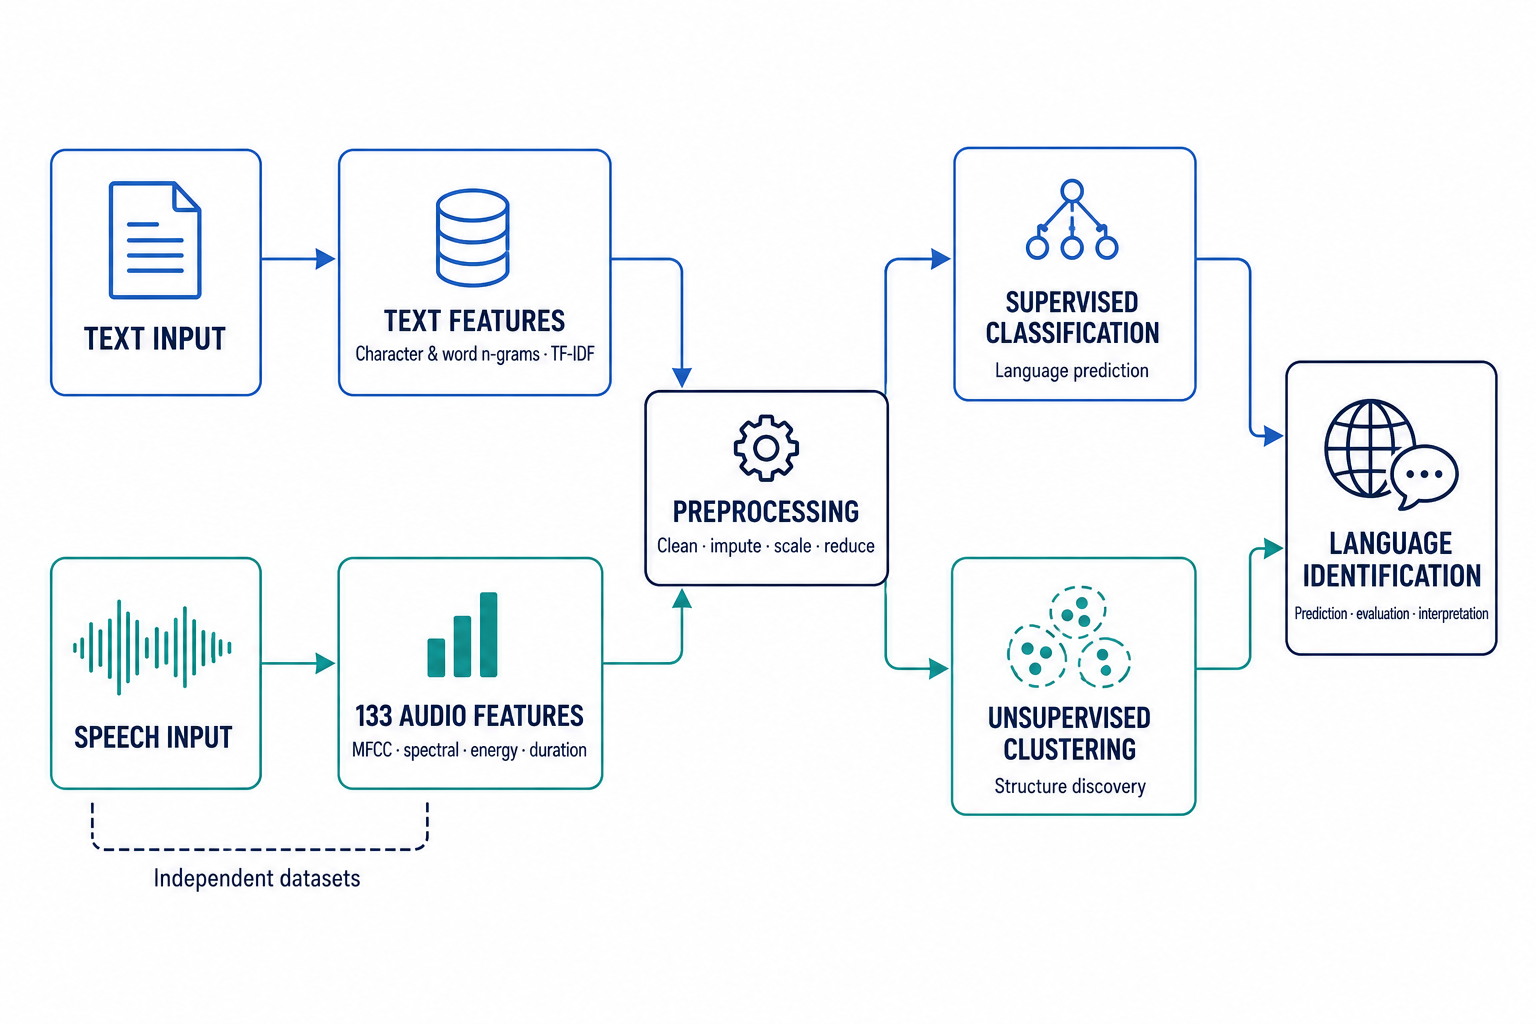
\includegraphics[width=\textwidth]
    {problem_statement_language_identification.png}
    \caption{نمای مفهومی مسئله تشخیص خودکار زبان در دو مسیر مستقل متن و گفتار}
    \label{fig:problem-statement-language-identification}
\end{figure}

در مسیر گفتار، فرایند مدل‌سازی از جدول
\lr{\texttt{features.csv}}
آغاز می‌شود. این جدول شامل ویژگی‌های عددی استخراج‌شده از نمونه‌های گفتاری است. بنابراین، پردازش فایل صوتی خام یا اجرای مجدد استخراج ویژگی، بخشی از خط لوله اصلی مدل‌سازی گفتار محسوب نمی‌شود.

در هر مسیر، چهار خانواده مستقل از الگوریتم‌های طبقه‌بندی و چهار خانواده مستقل از الگوریتم‌های خوشه‌بندی اجرا می‌شوند. تغییر یک پارامتر از یک الگوریتم به‌عنوان یک خانواده جدید در نظر گرفته نشده است.

در بخش طبقه‌بندی، مدل‌ها با استفاده از داده‌های برچسب‌دار آموزش داده می‌شوند. انتخاب مدل و تنظیم پارامترها فقط با استفاده از داده‌های آموزشی و اعتبارسنجی متقابل انجام می‌شود و داده آزمون نهایی در فرایند تنظیم مدل دخالت ندارد.

در بخش خوشه‌بندی، برچسب زبان هنگام برازش مدل‌ها مورد استفاده قرار نمی‌گیرد. برچسب‌ها تنها پس از تشکیل خوشه‌ها و برای محاسبه معیارهای خارجی و تفسیر نتایج به کار می‌روند.

جزئیات نظری ویژگی‌ها، الگوریتم‌ها و معیارهای ارزیابی در فصل دوم و جزئیات پیاده‌سازی و نتایج در فصل‌های بعدی ارائه خواهند شد.


% =================================================
\section{محدوده داده‌های پروژه}
% =================================================

این پروژه از دو مجموعه‌داده مستقل استفاده می‌کند که هرکدام دارای ساختار و کلاس‌های مخصوص خود هستند.


\subsection{مجموعه‌داده متنی}

مجموعه‌داده متنی شامل
\lr{608}
سند مستقل با کدگذاری
\lr{UTF--8}
است. این اسناد به شش زبان تعلق دارند:

\begin{itemize}

	\item آلمانی؛

	\item ایتالیایی؛

	\item ژاپنی؛

	\item کره‌ای؛

	\item پرتغالی؛

	\item اسپانیایی.

\end{itemize}

برچسب زبان از ساختار پوشه‌های مجموعه‌داده استخراج می‌شود. محتوای کامل هر فایل به‌عنوان متن نمونه در نظر گرفته شده است. پاک‌سازی متن به شکلی انجام می‌شود که نوع خط، حروف، نشانه‌گذاری، اعداد و علائم زبانی حفظ شوند.


\subsection{مجموعه‌داده گفتاری}

مجموعه‌داده گفتاری شامل
\lr{720}
نمونه و
\lr{133}
ویژگی عددی پیش‌بین است. این مجموعه چهار زبان را پوشش می‌دهد:

\begin{itemize}

	\item آلمانی؛

	\item اسپانیایی؛

	\item ایتالیایی؛

	\item کره‌ای.

\end{itemize}

برای هر زبان
\lr{180}
نمونه وجود دارد؛ بنابراین مجموعه‌داده گفتاری از نظر تعداد نمونه‌های هر کلاس متوازن است.

ویژگی‌های گفتاری در یک مرحله مستقل و پیش از شروع مدل‌سازی استخراج شده‌اند. پروژه حاضر این جدول ویژگی را اعتبارسنجی کرده و سپس برای تقسیم داده، پیش‌پردازش، آموزش مدل و ارزیابی استفاده می‌کند.

شناسه فایل، جنسیت و برچسب زبان به‌عنوان ویژگی پیش‌بین وارد مدل نمی‌شوند. همچنین، گروه‌های مرتبط با گوینده یا منبع داده در تقسیم آموزش و آزمون از یکدیگر جدا نگه داشته می‌شوند تا احتمال نشت اطلاعات کاهش یابد.


% =================================================
\section{اهداف پروژه}
% =================================================

هدف اصلی پروژه، طراحی و پیاده‌سازی یک چارچوب قابل تکرار برای
\textbf{شناسایی خودکار زبان از دو مجموعه‌داده مستقل متنی و گفتاری با استفاده از روش‌های یادگیری ماشین}
است.

برای دستیابی به این هدف، اهداف فرعی زیر در نظر گرفته شده‌اند:

\begin{itemize}

	\item کشف و اعتبارسنجی ساختار واقعی مجموعه‌داده متنی؛

	\item پاک‌سازی متن بدون حذف اطلاعات زبانی مهم مانند نوع خط، اعراب، نشانه‌ها و حروف خاص؛

	\item استخراج ویژگی‌های کاراکتری و واژگانی از متن با استفاده از
	\lr{TF--IDF}؛

	\item اعتبارسنجی جدول ویژگی‌های گفتاری بدون تغییر در فایل‌های ورودی؛

	\item جلوگیری از ورود شناسه‌ها، اطلاعات جانبی و برچسب زبان به ویژگی‌های پیش‌بین؛

	\item ایجاد تقسیم آموزش و آزمون به‌صورت گروه‌آگاه برای کاهش نشت اطلاعات؛

	\item آموزش، تنظیم و مقایسه دقیقاً چهار خانواده الگوریتم طبقه‌بندی برای هر مسیر؛

	\item اجرای دقیقاً چهار خانواده الگوریتم خوشه‌بندی برای هر مسیر؛

	\item انجام اعتبارسنجی متقابل و تنظیم ابرپارامترها فقط روی داده‌های آموزشی؛

	\item نگهداری داده آزمون نهایی خارج از فرایند انتخاب و تنظیم مدل؛

	\item ارزیابی طبقه‌بندی با استفاده از معیارهای
	\lr{Accuracy}،
	\lr{Precision}،
	\lr{Recall}
	و
	\lr{F1-score}؛

	\item تولید ماتریس درهم‌ریختگی و گزارش کامل طبقه‌بندی برای هر مدل؛

	\item ارزیابی خوشه‌بندی با معیارهای داخلی و معیارهای خارجی پس از برازش؛

	\item ذخیره مدل‌های آموزش‌دیده، پیش‌بینی‌ها، معیارها، نمودارها و تخصیص خوشه‌ها؛

	\item فراهم‌کردن امکان استنتاج زبان برای ورودی‌های جدید؛

	\item ایجاد یک روند اجرایی قابل تکرار با استفاده از محیط مدیریت‌شده
	\lr{Poetry}.

\end{itemize}

در مسیر متنی، هدف اصلی بررسی میزان توانایی الگوهای کاراکتری و واژگانی در تفکیک شش زبان موجود در مجموعه‌داده است.

در مسیر گفتاری نیز هدف بررسی میزان توانایی ویژگی‌های عددی استخراج‌شده از سیگنال صوتی در تفکیک چهار زبان آلمانی، اسپانیایی، ایتالیایی و کره‌ای است.

علاوه بر پیش‌بینی نظارت‌شده زبان، روش‌های بدون نظارت نیز بررسی می‌شوند تا مشخص شود آیا نمونه‌ها بدون استفاده از برچسب زبان در مرحله برازش، ساختار خوشه‌ای معناداری ایجاد می‌کنند یا خیر.


% =================================================
\section{کاربردهای شناسایی زبان}
% =================================================

سامانه‌های شناسایی خودکار زبان در بسیاری از حوزه‌های پردازش متن و گفتار کاربرد دارند. یکی از مهم‌ترین کاربردهای آن‌ها، استفاده به‌عنوان مرحله اولیه در سامانه‌های چندزبانه است.

برای مثال، در یک سامانه ترجمه ماشینی ممکن است کاربر متنی را بدون مشخص‌کردن زبان آن وارد کند. در چنین شرایطی، سامانه می‌تواند ابتدا زبان متن را شناسایی کرده و سپس مدل ترجمه مناسب را انتخاب کند.

در سامانه‌های پردازش گفتار نیز می‌توان پیش از اجرای مدل تبدیل گفتار به متن، زبان گوینده را تشخیص داد و مدل متناسب با آن زبان را فعال کرد.

از دیگر کاربردهای شناسایی خودکار زبان می‌توان به موارد زیر اشاره کرد:

\begin{itemize}

	\item سامانه‌های ترجمه ماشینی؛

	\item سامانه‌های تبدیل گفتار به متن؛

	\item دستیارهای صوتی چندزبانه؛

	\item دسته‌بندی خودکار اسناد و متون؛

	\item مسیریابی درخواست‌ها در سامانه‌های چندزبانه؛

	\item جست‌وجو و بازیابی اطلاعات چندزبانه؛

	\item تحلیل محتوای شبکه‌های اجتماعی؛

	\item مراکز تماس و سامانه‌های پاسخ‌گویی خودکار؛

	\item مدیریت مجموعه‌های بزرگ فایل‌های متنی و گفتاری؛

	\item تفکیک خودکار محتوای متعلق به زبان‌های مختلف.

\end{itemize}

در بسیاری از این کاربردها، شناسایی زبان تنها یک خروجی مستقل نیست، بلکه مرحله‌ای مقدماتی برای انتخاب روش پردازش مناسب در مراحل بعدی محسوب می‌شود. بنابراین، خطا در تشخیص زبان می‌تواند به انتخاب مدل نامناسب و کاهش کیفیت کل سامانه منجر شود.


% =================================================
\section{ابزارها و فناوری‌های مورد استفاده}
% =================================================

پیاده‌سازی پروژه با استفاده از زبان برنامه‌نویسی
\lr{\textbf{Python 3.12}}
انجام شده است. پایتون به دلیل برخورداری از کتابخانه‌های مناسب برای پردازش داده، یادگیری ماشین و پیاده‌سازی آزمایش‌های قابل تکرار، زبان اصلی این پروژه است.

مدیریت محیط و وابستگی‌های پروژه با استفاده از
\lr{\textbf{Poetry}}
انجام شده است. نسخه کتابخانه‌ها در فایل
\lr{\texttt{poetry.lock}}
ثبت شده‌اند تا اجرای مجدد پروژه در یک محیط مشابه امکان‌پذیر باشد.

کدهای قابل استفاده مجدد در ساختار
\lr{\texttt{src/}}
قرار دارند. اسکریپت‌های اجرایی در پوشه
\lr{\texttt{scripts/}}
مسئول اجرای مراحل مختلف خط لوله هستند و نوت‌بوک‌های
\lr{Jupyter}
برای توضیح مراحل، اجرای تحلیل‌ها و نمایش خروجی‌ها استفاده می‌شوند.

کتابخانه‌ها و ابزارهای اصلی پروژه عبارت‌اند از:


\subsection*{\lr{Pandas}}

کتابخانه
\lr{Pandas}
برای خواندن، مدیریت، پاک‌سازی، تبدیل و ذخیره داده‌های جدولی مورد استفاده قرار گرفته است.


\subsection*{\lr{NumPy}}

کتابخانه
\lr{NumPy}
برای انجام محاسبات عددی و کار با آرایه‌ها و ماتریس‌ها استفاده شده است.


\subsection*{\lr{Scikit-learn}}

کتابخانه
\lr{Scikit-learn}
برای پیاده‌سازی مراحل استخراج ویژگی متن، انتخاب ویژگی، پیش‌پردازش، تقسیم گروه‌آگاه داده، اعتبارسنجی متقابل، تنظیم ابرپارامترها، طبقه‌بندی، خوشه‌بندی، کاهش ابعاد و ارزیابی نتایج مورد استفاده قرار گرفته است.


\subsection*{\lr{SciPy}}

کتابخانه
\lr{SciPy}
برای پشتیبانی از محاسبات علمی و عملیات مرتبط با نمایش‌های عددی و تنک مورد استفاده قرار گرفته است.


\subsection*{\lr{Matplotlib}}

کتابخانه
\lr{Matplotlib}
برای تولید ماتریس‌های درهم‌ریختگی، نمودارهای مقایسه مدل‌ها و نمایش دوبعدی نتایج خوشه‌بندی استفاده شده است.


\subsection*{\lr{Jupyter Notebook}}

نوت‌بوک‌های
\lr{Jupyter}
برای اجرای مرحله‌به‌مرحله خط لوله، نمایش جداول و نمودارها و مستندسازی نتایج استفاده شده‌اند. منطق اصلی و قابل استفاده مجدد پروژه در ماژول‌های پوشه
\lr{\texttt{src/}}
قرار دارد و نوت‌بوک‌ها از این ماژول‌ها استفاده می‌کنند.


\subsection*{\lr{Joblib}}

کتابخانه
\lr{Joblib}
برای ذخیره و بارگذاری مدل‌های آموزش‌دیده، ابزارهای پیش‌پردازش و بسته‌های مورد نیاز برای استنتاج استفاده شده است.


\subsection*{\lr{PyYAML}}

کتابخانه
\lr{PyYAML}
برای خواندن تنظیمات متمرکز پروژه از فایل‌های پیکربندی استفاده شده است.


\subsection*{\lr{Pytest}}

ابزار
\lr{Pytest}
برای اجرای آزمون‌های خودکار مربوط به داده، تقسیم‌بندی، استخراج ویژگی، شمارش خانواده‌های مدل و استنتاج مورد استفاده قرار گرفته است.

پروژه به‌صورت محلی و روی
\lr{CPU}
قابل اجرا است و برای خط پایه آن نیازی به
\lr{GPU}
یا سرویس‌های ابری و پولی وجود ندارد. همچنین، چون مسیر گفتار از جدول ویژگی‌های از پیش استخراج‌شده آغاز می‌شود،
\lr{Librosa}
و
\lr{FFmpeg}
جزو وابستگی‌های الزامی خط لوله فعلی نیستند.


% =================================================
\section{نمای کلی معماری سیستم}
% =================================================

معماری پروژه به‌گونه‌ای طراحی شده است که منطق پردازش داده، آموزش مدل و ارزیابی از نوت‌بوک‌ها و اسکریپت‌های اجرایی جدا باشد.

اجزای اصلی پروژه عبارت‌اند از:

\begin{itemize}

	\item پوشه
	\lr{\texttt{src/}}
	برای نگهداری منطق اصلی و توابع قابل استفاده مجدد؛

	\item پوشه
	\lr{\texttt{scripts/}}
	برای اجرای مراحل مختلف پروژه از طریق خط فرمان؛

	\item پوشه
	\lr{\texttt{notebooks/}}
	برای توضیح، اجرای مرحله‌ای و نمایش نتایج؛

	\item پوشه
	\lr{\texttt{configs/}}
	برای نگهداری مسیرها، پارامترها و تنظیمات قابل تکرار؛

	\item پوشه
	\lr{\texttt{artifacts/}}
	برای ذخیره مدل‌ها، معیارها، جداول، پیش‌بینی‌ها، تخصیص خوشه‌ها و نمودارهای تولیدشده؛

	\item پوشه
	\lr{\texttt{tests/}}
	برای آزمون‌های خودکار پروژه.

\end{itemize}

این جداسازی باعث می‌شود که منطق اصلی پروژه فقط به اجرای یک نوت‌بوک خاص وابسته نباشد و مراحل مختلف بتوانند از طریق اسکریپت‌ها یا نوت‌بوک‌ها اجرا شوند.


% =================================================
\section{نمای کلی روند اجرای پروژه}
% =================================================

پروژه از دو خط لوله مستقل تشکیل شده است. اگرچه هر دو مسیر در نهایت به طبقه‌بندی و خوشه‌بندی منتهی می‌شوند، ورودی و مراحل آماده‌سازی آن‌ها متفاوت است.


\subsection{روند اجرای مسیر متن}

روند کلی مسیر متن به‌صورت زیر است:

\begin{center}
\textbf{
فایل‌های متنی خام
$\longleftarrow$
کشف و اعتبارسنجی داده
$\longleftarrow$
پاک‌سازی متن
$\longleftarrow$
استخراج ویژگی
$\longleftarrow$
طبقه‌بندی و خوشه‌بندی
$\longleftarrow$
ارزیابی و ذخیره نتایج
}
\end{center}

در مرحله نخست، فایل‌های متنی و ساختار پوشه‌ها بررسی می‌شوند. سپس متن‌ها با حفظ اطلاعات زبانی پاک‌سازی می‌شوند.

در مسیر طبقه‌بندی، نمایش متنی با ترکیب ویژگی‌های کاراکتری و واژگانی
\lr{TF--IDF}
ساخته می‌شود. پس از آن، ویژگی‌های مناسب با استفاده از روش
\lr{Chi-square}
انتخاب شده و چهار خانواده طبقه‌بندی با اعتبارسنجی متقابل گروه‌آگاه تنظیم و مقایسه می‌شوند.

در مسیر خوشه‌بندی، ویژگی‌های متنی بدون استفاده از برچسب زبان ساخته می‌شوند. سپس برای ایجاد یک نمایش فشرده‌تر از
\lr{Truncated SVD}
استفاده شده و چهار الگوریتم
\lr{K-Means}،
\lr{DBSCAN}،
\lr{Agglomerative Clustering}
و
\lr{Gaussian Mixture}
روی داده‌ها اجرا می‌شوند.


\subsection{روند اجرای مسیر گفتار}

روند کلی مسیر گفتار به‌صورت زیر است:

\begin{center}
\textbf{
جدول ویژگی‌های گفتاری
$\longleftarrow$
اعتبارسنجی داده و طرح‌واره
$\longleftarrow$
تقسیم گروه‌آگاه
$\longleftarrow$
پیش‌پردازش عددی
$\longleftarrow$
طبقه‌بندی و خوشه‌بندی
$\longleftarrow$
ارزیابی و ذخیره نتایج
}
\end{center}

در این مسیر، جدول ویژگی‌های از پیش استخراج‌شده بدون تغییر مورد استفاده قرار می‌گیرد. ابتدا ساختار جدول، مقادیر گمشده، مقادیر نامتناهی، ستون هدف، شناسه‌ها و ویژگی‌های عددی بررسی می‌شوند.

پس از اعتبارسنجی، داده‌ها با حفظ استقلال گروه‌های مربوط به گوینده یا منبع، به بخش‌های آموزش و آزمون تقسیم می‌شوند. پیش‌پردازش نظارت‌شده درون خط لوله آموزش مدل قرار می‌گیرد تا اطلاعات داده آزمون وارد فرایند یادگیری نشود.

برای خوشه‌بندی گفتار نیز برچسب زبان هنگام پیش‌پردازش، کاهش ابعاد، انتخاب پارامتر یا برازش الگوریتم استفاده نمی‌شود.


\subsection{روند ارزیابی}

در بخش طبقه‌بندی، مدل‌ها با استفاده از معیارهای زیر ارزیابی می‌شوند:

\begin{itemize}

	\item
	\lr{Accuracy}؛

	\item
	\lr{Macro Precision}؛

	\item
	\lr{Macro Recall}؛

	\item
	\lr{Macro F1-score}؛

	\item
	\lr{Weighted F1-score}؛

	\item ماتریس درهم‌ریختگی؛

	\item گزارش کامل طبقه‌بندی برای هر کلاس.

\end{itemize}

در بخش خوشه‌بندی، معیارهای داخلی مانند
\lr{Silhouette Score}،
\lr{Calinski--Harabasz}
و
\lr{Davies--Bouldin}
بدون نیاز به برچسب زبان محاسبه می‌شوند.

پس از برازش، از معیارهای
\lr{ARI}،
\lr{NMI}
و خلوص خوشه‌ها برای تفسیر میزان انطباق خوشه‌ها با زبان‌های واقعی استفاده می‌شود. این معیارهای خارجی در آموزش مدل یا انتخاب پارامترهای خوشه‌بندی دخالت ندارند.

در پایان، مدل‌های برتر، پیش‌پردازش‌های مورد نیاز برای استنتاج، جداول مقایسه، نمودارها و نتایج ماشین‌خوان ذخیره می‌شوند.

به این ترتیب، فصل حاضر تصویری کلی از مسئله، اهداف، محدوده داده‌ها، ابزارها و معماری پروژه ارائه داد. مبانی نظری ویژگی‌ها، الگوریتم‌ها و معیارهای ارزیابی در فصل دوم بررسی شده و جزئیات داده‌ها، پیاده‌سازی و نتایج آزمایش‌ها در فصل‌های بعد ارائه خواهند شد.


















% -------------------------------------------------
% فصل 2
% -------------------------------------------------

\projectchapter{مبانی نظری و مفاهیم پایه}{
در این فصل مفاهیم نظری و پیش‌زمینه‌های مورد نیاز برای درک روش‌های استفاده‌شده در پروژه بررسی می‌شوند. ابتدا مسئله شناسایی زبان از متن و گفتار معرفی شده و سپس مفاهیم یادگیری نظارت‌شده و بدون نظارت، روش‌های استخراج ویژگی از متن و صوت، الگوریتم‌های طبقه‌بندی و خوشه‌بندی، روش‌های کاهش ابعاد و در نهایت معیارهای ارزیابی مورد استفاده تشریح می‌شوند.
}


% =================================================
\section{مقدمه}
% =================================================

شناسایی خودکار زبان یکی از مسائل مهم در حوزه پردازش زبان طبیعی و پردازش گفتار محسوب می‌شود. هدف اصلی در این مسئله، تعیین زبان یک نمونه ورودی براساس ویژگی‌های قابل استخراج از آن است. ورودی سیستم می‌تواند یک متن یا یک فایل صوتی باشد.

اگر مجموعه زبان‌های موجود به صورت

\begin{equation}
L=\{L_1,L_2,\ldots,L_K\}
\end{equation}

تعریف شود، هدف سیستم یافتن تابعی است که برای یک نمونه ورودی $x$، یکی از زبان‌های مجموعه $L$ را انتخاب کند:

\begin{equation}
f(x)\longrightarrow L_i
\end{equation}

در این پروژه مسئله شناسایی زبان در دو حوزه متن و گفتار بررسی شده است. اگرچه هدف نهایی در هر دو بخش یکسان است، اما نوع داده و نحوه استخراج ویژگی در آن‌ها متفاوت است.

در ادامه این فصل، مفاهیم و روش‌هایی که مستقیماً در پیاده‌سازی پروژه استفاده شده‌اند مورد بررسی قرار می‌گیرند.


% =================================================
\section{شناسایی زبان از متن و گفتار}
% =================================================

\subsection{شناسایی زبان از متن}

در شناسایی زبان مبتنی بر متن\footnote{\lr{Text Language Identification}}، هدف تعیین زبان یک متن براساس ساختار نوشتاری آن است. زبان‌های مختلف از نظر نوع حروف، ساختار واژگان، ترکیب کاراکترها، فراوانی کلمات و ترتیب آن‌ها دارای الگوهای متفاوتی هستند.

حتی زبان‌هایی که از الفبای مشابه استفاده می‌کنند، معمولاً در نحوه قرارگیری حروف و ساختار کلمات تفاوت‌هایی دارند. به همین دلیل می‌توان با استخراج الگوهای آماری از متن، زبان آن را تشخیص داد.

در این پروژه برای نمایش عددی متون از ترکیب ویژگی‌های سطح کلمه و سطح کاراکتر استفاده شده است. این ویژگی‌ها با استفاده از روش
\lr{TF-IDF}
استخراج می‌شوند.


\subsection{شناسایی زبان از گفتار}

در شناسایی زبان از گفتار\footnote{\lr{Spoken Language Identification}}، ورودی سیستم یک سیگنال صوتی است.

یک سیگنال صوتی دیجیتال را می‌توان به صورت دنباله‌ای از نمونه‌ها نمایش داد:

\begin{equation}
x[n], \qquad n=0,1,\ldots,N-1
\end{equation}

که در آن $x[n]$ مقدار دامنه سیگنال در نمونه $n$ است.

استفاده مستقیم از تمام نمونه‌های سیگنال به عنوان ورودی مدل‌های کلاسیک یادگیری ماشین مناسب نیست؛ زیرا هر فایل ممکن است شامل تعداد بسیار زیادی نمونه باشد و همچنین طول فایل‌ها نیز یکسان نباشد.

بنابراین لازم است هر فایل صوتی به یک بردار ویژگی با طول ثابت تبدیل شود. در این پروژه این کار با استخراج مجموعه‌ای از ویژگی‌های طیفی، زمانی و انرژی انجام شده است.


% =================================================
\section{یادگیری ماشین در مسئله شناسایی زبان}
% =================================================

یادگیری ماشین را می‌توان به روش‌های مختلف تقسیم‌بندی کرد. در این پروژه از دو رویکرد اصلی استفاده شده است:

\begin{itemize}
	\item یادگیری نظارت‌شده؛
	\item یادگیری بدون نظارت.
\end{itemize}


% -------------------------------------------------
\subsection{یادگیری نظارت‌شده}
% -------------------------------------------------

در یادگیری نظارت‌شده\footnote{\lr{Supervised Learning}}، برای هر نمونه ورودی یک برچسب صحیح مشخص است.

مجموعه داده آموزشی را می‌توان به صورت زیر نمایش داد:

\begin{equation}
D=
\{(x_1,y_1),(x_2,y_2),\ldots,(x_N,y_N)\}
\end{equation}

که در آن:

\begin{itemize}
	\item $x_i$ بردار ویژگی نمونه $i$؛
	\item $y_i$ برچسب زبان نمونه؛
	\item $N$ تعداد نمونه‌ها است.
\end{itemize}

مدل با استفاده از این داده‌ها رابطه میان ویژگی‌ها و زبان واقعی را یاد گرفته و سپس زبان نمونه‌های جدید را پیش‌بینی می‌کند.

مسئله طبقه‌بندی\footnote{\lr{Classification}} مورد استفاده در این پروژه در این گروه قرار می‌گیرد.


% -------------------------------------------------
\subsection{یادگیری بدون نظارت}
% -------------------------------------------------

در یادگیری بدون نظارت\footnote{\lr{Unsupervised Learning}}، برچسب واقعی نمونه‌ها در اختیار الگوریتم قرار نمی‌گیرد.

در این حالت مجموعه داده به صورت

\begin{equation}
D=\{x_1,x_2,\ldots,x_N\}
\end{equation}

تعریف می‌شود.

الگوریتم تلاش می‌کند نمونه‌های مشابه را براساس ساختار ویژگی‌های آن‌ها در گروه‌هایی قرار دهد. این فرایند در مسئله خوشه‌بندی\footnote{\lr{Clustering}} مورد استفاده قرار می‌گیرد.

در این پروژه، خوشه‌بندی برای بررسی این موضوع انجام شده است که آیا نمونه‌های متعلق به یک زبان، بدون در اختیار داشتن برچسب زبان، به صورت طبیعی در کنار یکدیگر قرار می‌گیرند یا خیر.


% =================================================
\section{استخراج ویژگی از داده‌های متنی}
% =================================================

الگوریتم‌های کلاسیک یادگیری ماشین نمی‌توانند متن خام را مستقیماً پردازش کنند. بنابراین لازم است متن به یک نمایش عددی تبدیل شود.

در این پروژه از روش
\lr{TF-IDF}
در کنار
\lr{Word N-Gram}
و
\lr{Character N-Gram}
استفاده شده است.


% -------------------------------------------------
\subsection{مفهوم \lr{N-Gram}}
% -------------------------------------------------

\lr{N-Gram}
به دنباله‌ای شامل $n$ عنصر متوالی گفته می‌شود. این عناصر می‌توانند کلمه یا کاراکتر باشند.

برای مثال، در کلمه

\begin{center}
\lr{language}
\end{center}

برخی
\lr{Character Bigram}
ها عبارت‌اند از:

\begin{center}
\lr{la,\ an,\ ng,\ gu,\ ua,\ ag,\ ge}
\end{center}

همچنین برای جمله

\begin{center}
\lr{this is a language}
\end{center}

برخی
\lr{Word Bigram}
ها شامل موارد زیر هستند:

\begin{center}
\lr{this is,\ is a,\ a language}
\end{center}

در پروژه حاضر از ویژگی‌های زیر استفاده شده است:

\begin{itemize}
	\item \lr{Character N-Gram} با مرتبه‌های 2 تا 4؛
	\item \lr{Word N-Gram} با مرتبه‌های 1 تا 2.
\end{itemize}

استفاده هم‌زمان از این دو نوع ویژگی باعث می‌شود هم اطلاعات مربوط به ساختار کلمات و هم الگوهای موجود در ترکیب حروف در اختیار مدل قرار گیرد.


% -------------------------------------------------
\subsection{روش \lr{TF-IDF}}
% -------------------------------------------------

روش
\lr{TF-IDF}\footnote{\lr{Term Frequency--Inverse Document Frequency}}
یکی از روش‌های متداول برای تبدیل متن به نمایش عددی است.

این روش از دو مؤلفه اصلی تشکیل شده است.


\subsubsection{\lr{Term Frequency}}

مؤلفه
\lr{Term Frequency}
میزان تکرار یک ویژگی $t$ در سند $d$ را اندازه‌گیری می‌کند.

در حالت ساده می‌توان نوشت:

\begin{equation}
TF(t,d)=\mathrm{count}(t,d)
\end{equation}

در پروژه حاضر از
\lr{Sublinear TF}
استفاده شده است. در این حالت برای فراوانی‌های غیرصفر داریم:

\begin{equation}
TF(t,d)=1+\log(\mathrm{count}(t,d))
\end{equation}

استفاده از لگاریتم باعث می‌شود تکرار بسیار زیاد یک ویژگی، اثر بیش از حدی بر مدل ایجاد نکند.


\subsubsection{\lr{Inverse Document Frequency}}

مؤلفه
\lr{IDF}
نشان می‌دهد یک ویژگی در مجموعه اسناد تا چه اندازه خاص یا عمومی است.

فرم هموارشده آن را می‌توان به صورت زیر نمایش داد:

\begin{equation}
IDF(t)
=
\log
\left(
\frac{1+N}{1+df(t)}
\right)
+1
\end{equation}

که در آن:

\begin{itemize}
	\item $N$ تعداد کل اسناد؛
	\item $df(t)$ تعداد اسنادی است که ویژگی $t$ در آن‌ها وجود دارد.
\end{itemize}

در نهایت مقدار
\lr{TF-IDF}
از رابطه زیر به دست می‌آید:

\begin{equation}
TFIDF(t,d)
=
TF(t,d)
\times
IDF(t)
\end{equation}

بنابراین ویژگی‌هایی که در یک متن اهمیت زیادی دارند ولی در تمام متون به شکل گسترده تکرار نمی‌شوند، وزن بیشتری دریافت می‌کنند.


% -------------------------------------------------
\subsection{ترکیب ویژگی‌های کاراکتری و کلمه‌ای}
% -------------------------------------------------

در پروژه، ویژگی‌های استخراج‌شده در سطح کاراکتر و کلمه با یکدیگر ترکیب شده‌اند.

اگر ماتریس ویژگی‌های کاراکتری را با $X_c$ و ماتریس ویژگی‌های واژگانی را با $X_w$ نمایش دهیم، نمایش ترکیبی به‌صورت زیر خواهد بود:

\begin{equation}
X=
\left[
X_c
\quad
X_w
\right]
\end{equation}

این ترکیب باعث می‌شود اطلاعات مربوط به ساختار کلمات و الگوهای موجود در توالی کاراکترها به‌صورت هم‌زمان در اختیار مدل قرار گیرد. تنظیمات دقیق بردارسازهای کاراکتری و واژگانی در فصل سوم ارائه خواهند شد.


% -------------------------------------------------
\subsection{انتخاب ویژگی با \lr{Chi-Square}}
% -------------------------------------------------

برای انتخاب ویژگی‌های مناسب در بخش طبقه‌بندی متن از آزمون
\lr{Chi-Square}
استفاده شده است.

رابطه کلی آزمون کای‌دو به‌صورت زیر تعریف می‌شود:

\begin{equation}
\chi^2
=
\sum
\frac{(O-E)^2}{E}
\end{equation}

که در آن:

\begin{itemize}

	\item $O$ مقدار مشاهده‌شده؛

	\item $E$ مقدار مورد انتظار است.

\end{itemize}

هرچه مقدار
$\chi^2$
برای یک ویژگی بیشتر باشد، وابستگی آماری آن ویژگی به برچسب زبان بیشتر است.

ازآنجاکه آزمون
\lr{Chi-Square}
به برچسب زبان نیاز دارد، این مرحله فقط در مسیر طبقه‌بندی متن استفاده شده و در خوشه‌بندی متن به کار نرفته است.

برای جلوگیری از نشت اطلاعات، انتخاب ویژگی باید فقط با استفاده از بخش آموزشی انجام شود. تعداد دقیق ویژگی‌های انتخاب‌شده و نحوه اجرای این مرحله در فصل سوم تشریح خواهند شد.

% =================================================
\section{استخراج ویژگی از داده‌های صوتی}
% =================================================

هدف از استخراج ویژگی صوتی، تبدیل سیگنال خام با طول متغیر به یک بردار عددی با طول ثابت است.

خانواده ویژگی‌های صوتی مورد استفاده در ادامه معرفی می‌شوند و تعداد و ساختار دقیق ویژگی‌های نسخه نهایی در فصل سوم ارائه خواهد شد.


% -------------------------------------------------
\subsection{ضرایب \lr{MFCC}}
% -------------------------------------------------

یکی از مهم‌ترین ویژگی‌های مورد استفاده در پردازش گفتار،
\lr{MFCC}\footnote{\lr{Mel-Frequency Cepstral Coefficients}}
است.

مقیاس
\lr{Mel}
برای نزدیک کردن نمایش فرکانس به نحوه درک انسان از صوت مورد استفاده قرار می‌گیرد.

تبدیل تقریبی فرکانس معمولی به مقیاس
\lr{Mel}
به صورت زیر است:

\begin{equation}
Mel(f)
=
2595
\log_{10}
\left(
1+\frac{f}{700}
\right)
\end{equation}

پس از محاسبه طیف و عبور آن از بانک فیلترهای
\lr{Mel}،
از لگاریتم انرژی فیلترها و سپس تبدیل کسینوسی گسسته استفاده می‌شود.

یک فرم کلی برای محاسبه ضریب
\lr{MFCC}
به صورت زیر است:

\begin{equation}
c_n
=
\sum_{k=1}^{K}
\log(M_k)
\cos
\left[
\frac{\pi n}{K}
\left(
k-\frac{1}{2}
\right)
\right]
\end{equation}

که در آن:

\begin{itemize}
	\item $M_k$ انرژی فیلتر \lr{Mel} شماره $k$؛
	\item $K$ تعداد فیلترها؛
	\item $c_n$ ضریب \lr{MFCC} است.
\end{itemize}

از آنجا که
\lr{MFCC}
برای فریم‌های مختلف سیگنال محاسبه می‌شود، برای تبدیل آن به ویژگی با طول ثابت، میانگین و انحراف معیار هر ضریب استخراج شده است.

میانگین ضریب $i$ برابر است با:

\begin{equation}
\mu_i
=
\frac{1}{T}
\sum_{t=1}^{T}
c_i(t)
\end{equation}

و انحراف معیار آن برابر است با:

\begin{equation}
\sigma_i
=
\sqrt{
\frac{1}{T}
\sum_{t=1}^{T}
(c_i(t)-\mu_i)^2
}
\end{equation}

% -------------------------------------------------
\subsection{\lr{Delta MFCC} و \lr{Delta-Delta MFCC}}
% -------------------------------------------------

\lr{MFCC}
وضعیت طیفی سیگنال را در هر لحظه نمایش می‌دهد، اما نحوه تغییر این ضرایب در طول زمان نیز می‌تواند اطلاعات مهمی در مورد گفتار ارائه دهد.

برای ثبت تغییرات زمانی از ویژگی‌های
\lr{Delta MFCC}
و
\lr{Delta-Delta MFCC}
استفاده شده است.

یک تقریب متداول برای
\lr{Delta}
به صورت زیر است:

\begin{equation}
\Delta c_t
=
\frac{
\sum_{n=1}^{N}
n(c_{t+n}-c_{t-n})
}{
2
\sum_{n=1}^{N}
n^2
}
\end{equation}

\lr{Delta}
بیانگر سرعت تغییر
\lr{MFCC}
و
\lr{Delta-Delta}
بیانگر تغییرات مرتبه دوم یا شتاب تغییر ضرایب است.

برای ضرایب
\lr{Delta}
و
\lr{Delta-Delta}
نیز میانگین و انحراف معیار محاسبه شده است.


% -------------------------------------------------
\subsection{\lr{Zero Crossing Rate}}
% -------------------------------------------------

نرخ عبور از صفر یا
\lr{Zero Crossing Rate}
تعداد دفعاتی را اندازه‌گیری می‌کند که علامت سیگنال در طول زمان تغییر می‌کند.

رابطه آن را می‌توان به صورت زیر نمایش داد:

\begin{equation}
ZCR
=
\frac{1}{2(N-1)}
\sum_{n=1}^{N-1}
\left|
\mathrm{sgn}(x[n])
-
\mathrm{sgn}(x[n-1])
\right|
\end{equation}

برای ساخت یک نمایش با طول ثابت می‌توان از میانگین و انحراف معیار
\lr{ZCR}
در فریم‌های مختلف استفاده کرد.


% -------------------------------------------------
\subsection{ویژگی‌های طیفی}
% -------------------------------------------------

علاوه بر
\lr{MFCC}،
تعدادی ویژگی برای توصیف شکل و توزیع انرژی طیف استخراج شده‌اند.


\subsubsection{\lr{Spectral Centroid}}

\lr{Spectral Centroid}
مرکز جرم طیف فرکانسی را نشان می‌دهد:

\begin{equation}
SC
=
\frac{
\sum_k f_k S_k
}{
\sum_k S_k
}
\end{equation}

که $f_k$ فرکانس و $S_k$ مقدار طیفی متناظر با آن است.

مقادیر بالاتر این ویژگی به معنی تمرکز بیشتر انرژی در فرکانس‌های بالاتر است.


\subsubsection{\lr{Spectral Rolloff}}

\lr{Spectral Rolloff}
فرکانسی است که درصد مشخصی از انرژی کل طیف در زیر آن قرار دارد.

اگر $f_r$ فرکانس
\lr{Rolloff}
باشد:

\begin{equation}
\sum_{f_k\leq f_r}S_k
\geq
\alpha
\sum_k S_k
\end{equation}

که $\alpha$ نسبت مشخصی از انرژی کل طیف است.


\subsubsection{\lr{Spectral Bandwidth}}

\lr{Spectral Bandwidth}
میزان پراکندگی طیف در اطراف
\lr{Spectral Centroid}
را مشخص می‌کند:

\begin{equation}
BW
=
\sqrt{
\frac{
\sum_k
S_k(f_k-SC)^2
}{
\sum_kS_k
}
}
\end{equation}


\subsubsection{\lr{Spectral Flatness}}

\lr{Spectral Flatness}
میزان تخت یا قله‌دار بودن طیف را اندازه‌گیری می‌کند.

این معیار از نسبت میانگین هندسی به میانگین حسابی طیف به دست می‌آید:

\begin{equation}
SF
=
\frac{
\left(
\prod_{k=1}^{K}S_k
\right)^{1/K}
}{
\frac{1}{K}
\sum_{k=1}^{K}S_k
}
\end{equation}

این ویژگی می‌تواند اطلاعاتی درباره میزان نویزگونه یا ساختاریافته بودن طیف ارائه دهد.


% -------------------------------------------------
\subsection{\lr{RMS Energy}}
% -------------------------------------------------

انرژی
\lr{RMS}
یا
\lr{Root Mean Square Energy}
برای اندازه‌گیری سطح انرژی سیگنال استفاده می‌شود.

رابطه آن به صورت زیر است:

\begin{equation}
RMS
=
\sqrt{
\frac{1}{N}
\sum_{n=0}^{N-1}
x[n]^2
}
\end{equation}

برای ساخت ویژگی‌های سطح فایل می‌توان از میانگین و انحراف معیار
\lr{RMS}
استفاده کرد.


% -------------------------------------------------
\subsection{مدت زمان فایل صوتی}
% -------------------------------------------------

مدت زمان فایل صوتی نیز به عنوان یک ویژگی در نظر گرفته شده است.

اگر تعداد نمونه‌های سیگنال برابر $N$ و نرخ نمونه‌برداری برابر $f_s$ باشد، مدت زمان از رابطه زیر به دست می‌آید:

\begin{equation}
Duration
=
\frac{N}{f_s}
\end{equation}


% =================================================
\section{الگوریتم‌های طبقه‌بندی}
% =================================================

در مسیر متن، الگوریتم‌های
\lr{K-Nearest Neighbors}،
\lr{Decision Tree}،
\lr{Logistic Regression}
و
\lr{Multinomial Naive Bayes}
بررسی شده‌اند. در مسیر گفتار نیز الگوریتم‌های
\lr{Logistic Regression}،
\lr{Support Vector Machine}،
\lr{Random Forest}
و
\lr{K-Nearest Neighbors}
مورد استفاده قرار گرفته‌اند. جزئیات تنظیمات و ابرپارامترهای این مدل‌ها در فصل چهارم ارائه خواهند شد.


% -------------------------------------------------
\subsection{\lr{Logistic Regression}}
% -------------------------------------------------

رگرسیون لجستیک\footnote{\lr{Logistic Regression}} با وجود نام آن، یکی از الگوریتم‌های متداول برای طبقه‌بندی است.

در مسئله چندکلاسه، احتمال تعلق نمونه $x$ به کلاس $k$ را می‌توان با تابع
\lr{Softmax}
نمایش داد:

\begin{equation}
P(y=k|x)
=
\frac{
e^{w_k^Tx+b_k}
}{
\sum_{j=1}^{K}
e^{w_j^Tx+b_j}
}
\end{equation}

کلاس دارای بیشترین احتمال به عنوان خروجی مدل انتخاب می‌شود:

\begin{equation}
\hat{y}
=
\arg\max_k
P(y=k|x)
\end{equation}

در هر دو مسیر متن و گفتار،
\lr{Logistic Regression}
به‌عنوان یک طبقه‌بند خطی مورد بررسی قرار گرفته است. منظم‌سازی برای کنترل پیچیدگی مدل و کاهش بیش‌برازش به کار می‌رود.


% -------------------------------------------------
\subsection{\lr{Multinomial Naive Bayes}}
% -------------------------------------------------

روش
\lr{Naive Bayes}
یک الگوریتم احتمالاتی مبتنی بر قضیه بیز است:

\begin{equation}
P(C|X)
=
\frac{
P(X|C)P(C)
}{
P(X)
}
\end{equation}

مدل
\lr{Multinomial Naive Bayes}
به‌ویژه برای داده‌های متنی و ویژگی‌های مبتنی بر فراوانی یا
\lr{TF-IDF}
کاربرد دارد.

در این روش از پارامتر هموارسازی
$\alpha$
برای جلوگیری از صفر شدن احتمال برخی ویژگی‌ها استفاده می‌شود.

این الگوریتم در پروژه برای طبقه‌بندی داده‌های متنی استفاده شده است.


% -------------------------------------------------
\subsection{\lr{Decision Tree}}
% -------------------------------------------------

درخت تصمیم\footnote{\lr{Decision Tree}} با تقسیم پیاپی فضای ویژگی‌ها، نمونه‌ها را به گروه‌های خالص‌تر تقسیم می‌کند.

یکی از معیارهای رایج برای محاسبه ناخالصی یک گره،
\lr{Gini Impurity}
است:

\begin{equation}
Gini
=
1-
\sum_{k=1}^{K}
p_k^2
\end{equation}

که $p_k$ نسبت نمونه‌های کلاس $k$ در گره مورد نظر است.

این الگوریتم در پروژه برای طبقه‌بندی متن استفاده شده است. کنترل پیچیدگی درخت می‌تواند احتمال بیش‌برازش را کاهش دهد.


% -------------------------------------------------
\subsection{\lr{Support Vector Machine}}
% -------------------------------------------------

ماشین بردار پشتیبان یا
\lr{SVM}\footnote{\lr{Support Vector Machine}}
یکی از الگوریتم‌های اصلی مورد استفاده در بخش گفتار است.

در حالت خطی، تابع تصمیم به صورت زیر تعریف می‌شود:

\begin{equation}
f(x)
=
w^\top x+b
\end{equation}

هدف
\lr{SVM}
یافتن مرزی است که فاصله میان نزدیک‌ترین نمونه‌های کلاس‌ها و مرز تصمیم را بیشینه کند.

برای داده‌هایی که کاملاً جداشدنی نیستند، از مفهوم حاشیه نرم استفاده می‌شود. تابع هدف آن را می‌توان به‌صورت زیر نوشت:

\begin{equation}
\min_{w,b,\xi}
\left(
\frac{1}{2}\|w\|_2^2
+
C\sum_{i=1}^{N}\xi_i
\right)
\quad
\text{\lr{s.t.}}
\quad
y_i(w^\top x_i+b)\geq 1-\xi_i,
\quad
\xi_i\geq 0
\end{equation}

پارامتر $C$ تعادل میان بزرگ‌بودن حاشیه و جریمه خطاهای آموزشی را کنترل می‌کند.

برای جداسازی غیرخطی می‌توان از تابع کرنل استفاده کرد. کرنل مورد استفاده در این پروژه،
\lr{RBF}
است:

\begin{equation}
K(x_i,x_j)
=
\exp
\left(
-\gamma
\|x_i-x_j\|_2^2
\right)
\end{equation}

پارامتر $\gamma$ محدوده اثر هر نمونه را کنترل می‌کند. مقادیر بررسی‌شده برای $C$ و $\gamma$ در فصل چهارم ارائه خواهند شد.


% -------------------------------------------------
\subsection{\lr{K-Nearest Neighbors}}
% -------------------------------------------------

الگوریتم
\lr{KNN}\footnote{\lr{K-Nearest Neighbors}}
کلاس نمونه جدید را براساس نزدیک‌ترین نمونه‌های آموزشی مشخص می‌کند.

یکی از معیارهای فاصله، فاصله اقلیدسی است:

\begin{equation}
d(x_i,x_j)
=
\sqrt{
\sum_{m=1}^{p}
(x_{im}-x_{jm})^2
}
\end{equation}

پس از محاسبه فاصله، $K$ نزدیک‌ترین همسایه انتخاب شده و کلاس براساس رأی آن‌ها تعیین می‌شود.

برای نمایش‌های متنی می‌توان از فاصله کسینوسی استفاده کرد:

\begin{equation}
d_{\mathrm{cosine}}(x_i,x_j)
=
1-
\frac{x_i^\top x_j}{\|x_i\|_2\|x_j\|_2}
\end{equation}

معیار فاصله و نحوه وزن‌دهی همسایه‌ها باید متناسب با نوع نمایش داده انتخاب شوند. جزئیات انتخاب‌های انجام‌شده در دو مسیر در فصل چهارم بیان خواهند شد.


% -------------------------------------------------
\subsection{\lr{Random Forest}}
% -------------------------------------------------

جنگل تصادفی\footnote{\lr{Random Forest}} یک روش
\lr{Ensemble}
است که از مجموعه‌ای از درخت‌های تصمیم استفاده می‌کند.

خروجی نهایی در مسئله طبقه‌بندی از رأی اکثریت درخت‌ها به دست می‌آید:

\begin{equation}
\hat{y}
=
\mathrm{mode}
\{
h_1(x),
h_2(x),
\ldots,
h_M(x)
\}
\end{equation}

استفاده از چندین درخت باعث کاهش حساسیت مدل به نویز و کاهش احتمال بیش‌برازش نسبت به یک درخت منفرد می‌شود.

این الگوریتم در پروژه برای طبقه‌بندی ویژگی‌های گفتاری استفاده شده است.


% =================================================
\section{الگوریتم‌های خوشه‌بندی}
% =================================================

در فرآیند خوشه‌بندی، برچسب واقعی زبان‌ها در مرحله آموزش الگوریتم‌ها استفاده نشده و این برچسب‌ها تنها پس از تشکیل خوشه‌ها برای ارزیابی کیفیت تفکیک زبان‌ها به کار گرفته شده‌اند.

% -------------------------------------------------
\subsection{\lr{K-Means}}
% -------------------------------------------------

الگوریتم
\lr{K-Means}
داده‌ها را به $K$ خوشه تقسیم می‌کند و تلاش می‌کند فاصله نمونه‌ها از مرکز خوشه مربوط به خود را حداقل کند.

تابع هدف به صورت زیر است:

\begin{equation}
J
=
\sum_{k=1}^{K}
\sum_{x_i\in C_k}
\|x_i-\mu_k\|^2
\end{equation}

که در آن:

\begin{itemize}
	\item $C_k$ خوشه شماره $k$؛
	\item $\mu_k$ مرکز خوشه است.
\end{itemize}


% -------------------------------------------------
\subsection{\lr{Hierarchical Clustering}}
% -------------------------------------------------

در
\lr{Agglomerative Hierarchical Clustering}
ابتدا هر نمونه به عنوان یک خوشه مستقل در نظر گرفته می‌شود.

سپس در هر مرحله دو خوشه نزدیک‌تر با یکدیگر ادغام می‌شوند تا در نهایت تعداد مورد نظر خوشه‌ها حاصل شود.

در روش
\lr{Ward Linkage}
ادغامی انتخاب می‌شود که کمترین افزایش را در واریانس داخل خوشه‌ها ایجاد کند.


% -------------------------------------------------
\subsection{\lr{Gaussian Mixture Model}}
% -------------------------------------------------

در بخش متنی و گفتاری پروژه از
\lr{Gaussian Mixture Model}
نیز استفاده شده است.

در این روش فرض می‌شود توزیع داده از ترکیب چند توزیع
\lr{Gaussian}
تشکیل شده باشد:

\begin{equation}
p(x)
=
\sum_{k=1}^{K}
\pi_k
\mathcal{N}
(x|\mu_k,\Sigma_k)
\end{equation}

که در آن:

\begin{itemize}
	\item $\pi_k$ وزن مؤلفه $k$؛
	\item $\mu_k$ بردار میانگین؛
	\item $\Sigma_k$ ماتریس کوواریانس است.
\end{itemize}

این روش برخلاف
\lr{K-Means}
امکان محاسبه احتمال تعلق هر نمونه به خوشه‌های مختلف را فراهم می‌کند.

یکی از معیارهای قابل استفاده برای انتخاب پیچیدگی مدل مخلوط گاوسی، معیار اطلاعات بیزی یا
\lr{BIC}\footnote{\lr{Bayesian Information Criterion}}
است:

\begin{equation}
BIC
=
-2\log(\hat{\mathcal{L}})
+
q\log(N)
\end{equation}

که در آن $\hat{\mathcal{L}}$ بیشینه درست‌نمایی و $q$ تعداد پارامترهای مدل است. مقدار کمتر این معیار نشان‌دهنده تعادل مناسب‌تر میان برازش و پیچیدگی مدل است.


% -------------------------------------------------
\subsection{\lr{DBSCAN}}
% -------------------------------------------------

الگوریتم
\lr{DBSCAN}\footnote{\lr{Density-Based Spatial Clustering of Applications with Noise}}
یک روش خوشه‌بندی مبتنی بر چگالی است.

دو پارامتر اصلی آن عبارت‌اند از:

\begin{itemize}
	\item \lr{eps} یا شعاع همسایگی؛
	\item \lr{min\_samples} یا حداقل تعداد نقاط همسایه.
\end{itemize}

یک نقطه در صورتی نقطه مرکزی محسوب می‌شود که:

\begin{equation}
|N_{\varepsilon}(x)|
\geq
MinPts
\end{equation}

یکی از مزایای مهم
\lr{DBSCAN}
قابلیت تشخیص نمونه‌های نویزی است که معمولاً با برچسب $-1$ مشخص می‌شوند.

% =================================================
\section{آماده‌سازی و کاهش ابعاد ویژگی‌ها}
% =================================================


% -------------------------------------------------
\subsection{استانداردسازی ویژگی‌ها}
% -------------------------------------------------

ویژگی‌های صوتی دارای مقیاس‌های عددی متفاوت هستند. این موضوع می‌تواند به‌ویژه بر الگوریتم‌های مبتنی بر فاصله اثرگذار باشد.

استانداردسازی یک ویژگی به‌صورت زیر تعریف می‌شود:

\begin{equation}
z
=
\frac{x-\mu}{\sigma}
\end{equation}

که در آن:

\begin{itemize}
	\item $\mu$ میانگین ویژگی؛
	\item $\sigma$ انحراف معیار ویژگی است.
\end{itemize}

پس از استانداردسازی، ویژگی‌ها دارای میانگین تقریباً صفر و انحراف معیار تقریباً یک خواهند بود.


% -------------------------------------------------
\subsection{\lr{Principal Component Analysis}}
% -------------------------------------------------

روش
\lr{PCA}\footnote{\lr{Principal Component Analysis}}
برای کاهش ابعاد و حذف هم‌بستگی میان ویژگی‌ها استفاده می‌شود.

اگر ماتریس کوواریانس داده را با $\Sigma$ نمایش دهیم:

\begin{equation}
\Sigma v_i
=
\lambda_i v_i
\end{equation}

که در آن:

\begin{itemize}
	\item $v_i$ بردار ویژه؛
	\item $\lambda_i$ مقدار ویژه متناظر است.
\end{itemize}

مؤلفه‌هایی که مقدار ویژه بزرگ‌تری دارند، بخش بیشتری از واریانس داده را توضیح می‌دهند.

در پروژه حاضر، این روش برای ایجاد نمایش کم‌بعد ویژگی‌های گفتاری در مسیر خوشه‌بندی استفاده شده است. تعداد مؤلفه‌ها و جزئیات اجرا در فصل سوم ارائه خواهند شد.


% -------------------------------------------------
\subsection{\lr{Truncated SVD}}
% -------------------------------------------------

ماتریس
\lr{TF-IDF}
معمولاً دارای تعداد ابعاد بالا و ساختاری
\lr{Sparse}
است.

در خوشه‌بندی متن از
\lr{Truncated SVD}
برای کاهش ابعاد فضای ویژگی استفاده شده است.

تجزیه
\lr{SVD}
به صورت زیر تعریف می‌شود:

\begin{equation}
X
=
U\Sigma V^T
\end{equation}

در نسخه
\lr{Truncated}
تنها تعداد محدودی از مؤلفه‌ها نگه داشته می‌شوند:

\begin{equation}
X
\approx
U_r
\Sigma_r
V_r^T
\end{equation}

این روش امکان کاهش ابعاد ماتریس
\lr{TF-IDF}
را بدون تبدیل مستقیم آن به یک ماتریس
\lr{Dense}
فراهم می‌کند.

در پروژه حاضر، این روش برای ایجاد نمایش کم‌بعد متن در مسیر خوشه‌بندی استفاده شده است. تعداد مؤلفه‌ها و نحوه نرمال‌سازی نمایش نهایی در فصل سوم بیان خواهند شد.


% =================================================
\section{تنظیم و اعتبارسنجی مدل}
% =================================================


% -------------------------------------------------
\subsection{\lr{Cross Validation}}
% -------------------------------------------------

برای ارزیابی قابل اعتمادتر مدل، از
\lr{Cross Validation}
استفاده شده است.

در این پروژه برای جلوگیری از قرار گرفتن نمونه‌های وابسته به یک منبع مشترک در بخش‌های مختلف آموزش و ارزیابی، از روش
\lr{Stratified Group K-Fold}
استفاده شده است.

در این روش علاوه بر حفظ نسبت نمونه‌های کلاس‌های مختلف در
\lr{Fold}
ها، نمونه‌های متعلق به یک گروه مشترک در یک بخش قرار می‌گیرند.

اگر امتیاز هر
\lr{Fold}
برابر $S_i$ باشد، امتیاز میانگین به صورت زیر محاسبه می‌شود:

\begin{equation}
CV
=
\frac{1}{K}
\sum_{i=1}^{K}
S_i
\end{equation}


% -------------------------------------------------
\subsection{\lr{Grid Search}}
% -------------------------------------------------

برای انتخاب بهترین مقادیر ابرپارامترها می‌توان از روش
\lr{Grid Search}
استفاده کرد.

این روش ترکیب‌های مختلف پارامترهای تعیین‌شده را آزمایش کرده و هر ترکیب را با استفاده از
\lr{Cross Validation}
ارزیابی می‌کند.

در این پروژه، معیارهایی مانند
\lr{Macro F1}
برای مقایسه مدل‌ها و انتخاب تنظیمات مناسب مورد استفاده قرار گرفته‌اند.

تعداد بخش‌های اعتبارسنجی و شبکه ابرپارامترهای هر مدل در فصل چهارم ارائه خواهند شد.

% =================================================
\section{معیارهای ارزیابی طبقه‌بندی}
% =================================================


% -------------------------------------------------
\subsection{\lr{Accuracy}}
% -------------------------------------------------

دقت کلی یا
\lr{Accuracy}
نسبت تعداد پیش‌بینی‌های صحیح به کل پیش‌بینی‌ها است. در حالت چندکلاسه می‌توان نوشت:

\begin{equation}
Accuracy
=
\frac{1}{N}
\sum_{i=1}^{N}
\mathbb{I}(y_i=\hat{y}_i)
\end{equation}


% -------------------------------------------------
\subsection{\lr{Precision}}
% -------------------------------------------------

معیار
\lr{Precision}
مشخص می‌کند از میان نمونه‌هایی که مدل به یک کلاس نسبت داده است، چه نسبتی واقعاً متعلق به آن کلاس بوده‌اند:

\begin{equation}
Precision
=
\frac{TP}{TP+FP}
\end{equation}


% -------------------------------------------------
\subsection{\lr{Recall}}
% -------------------------------------------------

\lr{Recall}
نشان می‌دهد چه نسبتی از نمونه‌های واقعی یک کلاس به درستی تشخیص داده شده‌اند:

\begin{equation}
Recall
=
\frac{TP}{TP+FN}
\end{equation}


% -------------------------------------------------
\subsection{\lr{F1-Score}}
% -------------------------------------------------

معیار
\lr{F1-Score}
میانگین هارمونیک
\lr{Precision}
و
\lr{Recall}
است:

\begin{equation}
F1
=
2
\frac{
Precision
\times
Recall
}{
Precision+Recall
}
\end{equation}


% -------------------------------------------------
\subsection{میانگین‌های \lr{Macro} و \lr{Weighted}}
% -------------------------------------------------

در میانگین
\lr{Macro}،
معیار برای هر کلاس به‌صورت مستقل محاسبه می‌شود و تمام کلاس‌ها وزن یکسانی دارند:

\begin{equation}
MacroPrecision
=
\frac{1}{K}
\sum_{k=1}^{K}Precision_k
\end{equation}

\begin{equation}
MacroRecall
=
\frac{1}{K}
\sum_{k=1}^{K}Recall_k
\end{equation}

\begin{equation}
MacroF1
=
\frac{1}{K}
\sum_{k=1}^{K}
F1_k
\end{equation}

در میانگین وزنی، سهم هر کلاس متناسب با تعداد نمونه‌های واقعی آن است. برای مثال:

\begin{equation}
WeightedF1
=
\sum_{k=1}^{K}
\frac{n_k}{N}F1_k
\end{equation}

که در آن $n_k$ تعداد نمونه‌های کلاس $k$ و $N$ تعداد کل نمونه‌ها است.


% -------------------------------------------------
\subsection{\lr{Confusion Matrix}}
% -------------------------------------------------

ماتریس درهم‌ریختگی\footnote{\lr{Confusion Matrix}} زبان واقعی نمونه‌ها را با زبان پیش‌بینی‌شده مقایسه می‌کند.

اگر $C_{ij}$ عضو سطر $i$ و ستون $j$ باشد:

\begin{equation}
C_{ij}
=
\text{تعداد نمونه‌های کلاس واقعی }i
\text{ که به کلاس }j
\text{ نسبت داده شده‌اند}
\end{equation}

مقادیر روی قطر اصلی نشان‌دهنده پیش‌بینی‌های صحیح و مقادیر خارج از قطر بیانگر خطاهای مدل هستند.


% =================================================
\section{معیارهای ارزیابی خوشه‌بندی}
% =================================================

معیارهای خوشه‌بندی به دو دسته داخلی و خارجی تقسیم می‌شوند. معیارهای داخلی فقط از ویژگی‌ها و تخصیص خوشه‌ها استفاده می‌کنند. معیارهای خارجی، مانند
\lr{ARI}،
\lr{NMI}
و
\lr{Purity}،
فقط پس از تشکیل خوشه‌ها و برای مقایسه با برچسب‌های واقعی به کار می‌روند.


% -------------------------------------------------
\subsection{\lr{Silhouette Score}}
% -------------------------------------------------

معیار
\lr{Silhouette Score}
برای بررسی انسجام داخل خوشه‌ها و میزان جدایی میان خوشه‌های مختلف استفاده می‌شود.

برای نمونه $i$:

\begin{itemize}
	\item $a(i)$ میانگین فاصله نمونه با اعضای خوشه خودش؛
	\item $b(i)$ کمترین میانگین فاصله نمونه با یک خوشه دیگر است.
\end{itemize}

در نتیجه:

\begin{equation}
s(i)
=
\frac{
b(i)-a(i)
}{
\max(a(i),b(i))
}
\end{equation}

و داریم:

\begin{equation}
-1
\leq
s(i)
\leq
1
\end{equation}

مقادیر نزدیک به 1 بیانگر کیفیت بهتر خوشه‌بندی هستند.

\subsection{\lr{Calinski-Harabasz Index}}

معیار
\lr{Calinski-Harabasz}
نسبت پراکندگی بین خوشه‌ها به پراکندگی درون خوشه‌ها را اندازه‌گیری می‌کند.

مقدار بالاتر این معیار نشان‌دهنده جدایی بهتر خوشه‌ها و فشردگی بیشتر نمونه‌های داخل هر خوشه است.

\subsection{\lr{Davies-Bouldin Index}}

معیار
\lr{Davies-Bouldin}
میزان شباهت میان هر خوشه و نزدیک‌ترین خوشه دیگر را بررسی می‌کند.

مقدار کمتر این معیار نشان‌دهنده کیفیت بهتر خوشه‌بندی است.
% -------------------------------------------------
\subsection{\lr{Cluster Purity}}
% -------------------------------------------------

معیار
\lr{Purity}
بررسی می‌کند اعضای هر خوشه تا چه اندازه به یک کلاس واقعی تعلق دارند.

اگر مجموعه خوشه‌ها برابر

\begin{equation}
\Omega
=
\{\omega_1,\ldots,\omega_K\}
\end{equation}

باشد،
\lr{Purity}
به صورت زیر تعریف می‌شود:

\begin{equation}
Purity(\Omega,C)
=
\frac{1}{N}
\sum_k
\max_j
|\omega_k\cap c_j|
\end{equation}

مقدار بیشتر
\lr{Purity}
نشان‌دهنده تطابق بیشتر خوشه‌ها با زبان‌های واقعی است.

این معیار به تعداد خوشه‌ها حساس است و ممکن است با تشکیل خوشه‌های کوچک‌تر افزایش یابد؛ بنابراین باید در کنار معیارهای دیگر تفسیر شود.


% -------------------------------------------------
\subsection{\lr{Adjusted Rand Index}}
% -------------------------------------------------

در بخش خوشه‌بندی، از
\lr{Adjusted Rand Index}
برای مقایسه ساختار خوشه‌های ایجادشده با برچسب‌های واقعی استفاده شده است.

فرم کلی این معیار به صورت زیر است:

\begin{equation}
ARI
=
\frac{
RI-E[RI]
}{
\max(RI)-E[RI]
}
\end{equation}

مقدار نزدیک به 1 بیانگر تطابق بالا میان خوشه‌بندی و برچسب‌های واقعی است.

مقدار یک نشان‌دهنده انطباق کامل، مقدار نزدیک به صفر نشان‌دهنده توافق مشابه حالت تصادفی و مقدار منفی نشان‌دهنده توافق کمتر از انتظار تصادفی است.


% -------------------------------------------------
\subsection{\lr{Normalized Mutual Information}}
% -------------------------------------------------

معیار
\lr{NMI}\footnote{\lr{Normalized Mutual Information}}
میزان اطلاعات مشترک میان تخصیص خوشه‌ها و برچسب‌های واقعی را اندازه‌گیری می‌کند. در نرمال‌سازی حسابی می‌توان نوشت:

\begin{equation}
NMI(C,Y)
=
\frac{2I(C;Y)}{H(C)+H(Y)}
\end{equation}

که در آن $I(C;Y)$ اطلاعات متقابل و $H(C)$ و $H(Y)$ آنتروپی خوشه‌ها و برچسب‌های واقعی هستند. مقدار این معیار در بازه صفر تا یک قرار می‌گیرد و مقدار بزرگ‌تر نشان‌دهنده انطباق بیشتر است.


% =================================================
\section{خلاصه و جمع‌بندی}
% =================================================

در این فصل مفاهیم نظری مورد نیاز برای درک مراحل پیاده‌سازی پروژه بررسی شدند. ابتدا مسئله شناسایی زبان از متن و گفتار و تفاوت میان یادگیری نظارت‌شده و بدون نظارت معرفی شد.

در بخش متن، روش‌های استخراج ویژگی شامل
\lr{Character N-Gram}،
\lr{Word N-Gram}،
\lr{TF-IDF}
و انتخاب ویژگی با
\lr{Chi-Square}
تشریح شدند. در بخش گفتار نیز نحوه استخراج ویژگی‌های
\lr{MFCC}،
\lr{Delta MFCC}،
\lr{Delta-Delta MFCC}،
ویژگی‌های طیفی، انرژی و مدت زمان بررسی شدند. تعداد و ساختار دقیق ویژگی‌های نسخه نهایی در فصل سوم ارائه خواهند شد.

همچنین الگوریتم‌های طبقه‌بندی و خوشه‌بندی مورد استفاده، روش‌های استانداردسازی و کاهش ابعاد،
\lr{Cross Validation}،
\lr{Grid Search}
و معیارهای ارزیابی معرفی شدند.

مفاهیم ارائه‌شده در این فصل، مبنای نظری مراحل آماده‌سازی داده، پیاده‌سازی مدل‌ها و تحلیل نتایج در فصل‌های بعدی خواهند بود.

































































































% -------------------------------------------------
% فصل 3 جدید
% -------------------------------------------------

\projectchapter{داده‌ها و پیش‌پردازش}{
در این فصل، دو مجموعه‌داده مستقل متنی و گفتاری پروژه معرفی شده و مراحل عملی آماده‌سازی آن‌ها تشریح می‌شود. ابتدا ساختار و توزیع داده‌های متنی، نحوه پاک‌سازی و تبدیل آن‌ها به فضای ویژگی بررسی شده و سپس فرایندی که برای استانداردسازی فایل‌های صوتی، تولید فراداده و استخراج ویژگی‌های گفتاری انجام شده است ارائه می‌شود. هدف این فصل، تشریح روند تبدیل داده‌های خام به ورودی‌های قابل استفاده برای مدل‌های یادگیری ماشین است.
}


% =================================================
\section{مقدمه}
% =================================================

کیفیت داده ورودی یکی از عوامل مهم در عملکرد مدل‌های یادگیری ماشین است. حتی در صورت انتخاب یک الگوریتم مناسب، وجود داده‌های ناسازگار، ناقص یا دارای ساختار نامناسب می‌تواند بر نتیجه نهایی تأثیر منفی بگذارد. به همین دلیل، پیش از مرحله آموزش مدل لازم است داده‌های خام بررسی، پاک‌سازی و به یک نمایش مناسب تبدیل شوند.

در پروژه حاضر، دو مجموعه‌داده با ساختارهای متفاوت مورد استفاده قرار گرفته است. بخش نخست شامل فایل‌های متنی در چند زبان مختلف و بخش دوم شامل داده‌های گفتاری است که پس از پاک‌سازی صوت و استخراج ویژگی در قالب جدول عددی ذخیره شده‌اند.

از آنجا که ماهیت این دو نوع داده متفاوت است، مراحل پیش‌پردازش آن‌ها نیز به صورت مستقل طراحی شده است. با این حال، در هر دو بخش هدف نهایی یکسان است: تبدیل داده خام به ساختاری عددی، منظم و قابل استفاده در الگوریتم‌های یادگیری ماشین.

مبانی نظری روش‌های استخراج ویژگی در فصل دوم تشریح شد؛ بنابراین در این فصل تمرکز اصلی بر داده‌های واقعی، نحوه پیاده‌سازی و پارامترهایی است که در نسخه نهایی پروژه مورد استفاده قرار گرفته‌اند. مراحل پاک‌سازی و استخراج ویژگی صوتی پیش‌تر توسط نگارنده اجرا و فایل‌های
\lr{features.csv}
و
\lr{metadata.csv}
تولید شده‌اند؛ خط لوله مدل‌سازی فعلی این دو فایل را به‌عنوان ورودی فقط‌خواندنی دریافت می‌کند و استخراج ویژگی صوتی را دوباره اجرا نمی‌کند.


% =================================================
\section{ساختار کلی داده‌های پروژه}
% =================================================

داده‌های پروژه در دو مجموعه مستقل سازمان‌دهی شده‌اند:

\begin{itemize}

	\item یک مجموعه مستقل از فایل‌های متنی برای شناسایی زبان از متن؛

	\item یک مجموعه گفتاری مستقل که فایل‌های صوتی پاک‌سازی‌شده، فراداده و جدول ویژگی‌های استخراج‌شده را در بر می‌گیرد.

\end{itemize}

در بخش متن، هر نمونه شامل یک فایل متنی، برچسب زبان و فراداده اختیاری استخراج‌شده از ساختار مسیر است. پس از بارگذاری و پاک‌سازی، متن‌ها به بردارهای عددی تبدیل می‌شوند.

در بخش گفتار نیز هر سطر از جدول نهایی با یک فایل صوتی متناظر است و شامل مسیر فایل، برچسب زبان، اطلاعات جنسیت گوینده و ویژگی‌های عددی استخراج‌شده است.

دو مجموعه داده به صورت مستقل پردازش شده‌اند. هیچ تطبیق سطربه‌سطر میان نمونه‌های متن و گفتار فرض نشده و هیچ ترکیب مستقیمی میان ویژگی‌های دو بخش در مرحله مدل‌سازی انجام نشده است؛ بنابراین نتایج آن‌ها نیز به‌عنوان یک آزمایش زوج‌شده تفسیر نمی‌شوند.


% =================================================
\section{آماده‌سازی داده‌های متنی}
% =================================================


% -------------------------------------------------
\subsection{ساختار و توزیع داده‌های متنی}
% -------------------------------------------------

مجموعه داده متنی نهایی شامل
\textbf{608 نمونه}
از شش زبان آلمانی، اسپانیایی، ایتالیایی، کره‌ای، پرتغالی و ژاپنی است.

ساختار پوشه‌های داده به شکلی طراحی شده است که هر زبان دارای یک کد اختصاصی باشد. نگاشت مورد استفاده در پروژه در جدول زیر ارائه شده است.
\begin{table}[H]
\centering
\caption{توزیع نمونه‌های مجموعه داده متنی}
\label{tab:text-data-distribution}
\begin{tabular}{c c c c}
\toprule
\textbf{زبان} &
\textbf{کد پوشه} &
\textbf{تعداد نمونه} &
\textbf{میانگین طول متن} \\
\midrule
آلمانی    & \lr{de} & \lr{104} & \lr{313.5} \\
اسپانیایی & \lr{es} & \lr{100} & \lr{313.8} \\
ایتالیایی & \lr{it} & \lr{106} & \lr{313.0} \\
کره‌ای    & \lr{ko} & \lr{98}  & \lr{318.3} \\
پرتغالی   & \lr{po} & \lr{100} & \lr{314.9} \\
ژاپنی     & \lr{ja} & \lr{100} & \lr{315.0} \\
\midrule
\textbf{مجموع} & \lr{--} & \textbf{\lr{608}} & \lr{--} \\
\bottomrule
\end{tabular}
\end{table}

همان‌طور که جدول \ref{tab:text-data-distribution} نشان می‌دهد، تعداد نمونه‌ها بین زبان‌های مختلف تقریباً متوازن است و اختلاف تعداد نمونه‌های کلاس‌ها محدود است.

میانگین طول متن در این جدول پس از یکسان‌سازی فاصله‌ها و برحسب تعداد کاراکتر محاسبه شده است.

این ویژگی اهمیت دارد، زیرا عدم توازن شدید میان کلاس‌ها می‌تواند باعث شود مدل در فرایند آموزش به سمت زبان‌هایی که تعداد نمونه بیشتری دارند متمایل شود.


% -------------------------------------------------
\subsection{بارگذاری و برچسب‌گذاری داده‌های متنی}
% -------------------------------------------------

برای بارگذاری داده‌ها از مسیر
\lr{\texttt{data/raw/text}}
استفاده شده است. تمام فایل‌های دارای پسوند
\lr{\texttt{.txt}}
به صورت بازگشتی از شش پوشه زبانی تعریف‌شده در فایل تنظیمات خوانده شده‌اند. نام پوشه نخست، کد زبان را مشخص می‌کند و سپس این کد به نام کامل زبان نگاشت می‌شود.

هر فایل متنی با کدگذاری
\lr{UTF-8}
و به‌صورت سخت‌گیرانه خوانده شده است؛ بنابراین در صورت رخ‌دادن خطای رمزگشایی، اجرا با پیام خطا متوقف می‌شود و کاراکتر نامعتبر به‌صورت خاموش حذف نمی‌شود. در اجرای نهایی، هر 608 فایل با موفقیت رمزگشایی شدند و هیچ کاراکتر جایگزین یونیکد در متن پاک‌سازی‌شده مشاهده نشد.

برای هر نمونه اطلاعات زیر ذخیره شده است:

\begin{itemize}

	\item شناسه نمونه شامل مسیر نسبی فایل؛

	\item زبان نمونه؛

	\item اطلاعات جنسیت استخراج‌شده از پوشه دوم، در صورت وجود؛

	\item متن خام و متن پاک‌سازی‌شده؛

	\item شناسه گروه مربوط به گوینده یا منبع نمونه.

\end{itemize}


% -------------------------------------------------
\subsection{پاک‌سازی متون}
% -------------------------------------------------

هدف اصلی مرحله پاک‌سازی، ایجاد یک نمایش یکنواخت از متن بدون حذف اطلاعاتی است که ممکن است برای تشخیص زبان مفید باشند.

پاک‌سازی مورد استفاده در این پروژه به صورت کنترل‌شده و حداقلی انجام شده است.

در این مرحله، تمام فاصله‌ها، خطوط جدید و
\lr{Tab}
های متوالی به یک فاصله واحد تبدیل شده و فاصله‌های ابتدا و انتهای متن حذف شده‌اند.

به صورت مفهومی عملیات انجام‌شده را می‌توان به شکل زیر نمایش داد:

\begin{center}
\lr{\texttt{Multiple Whitespaces}}
$\longleftarrow$
\lr{\texttt{Single Space}}
\end{center}

برخلاف برخی مسائل پردازش متن، در این پروژه کاراکترهای خاص زبان‌ها حذف نشده‌اند. همچنین علائم نگارشی، اعداد، حروف دارای
\lr{Accent}،
\lr{Umlaut}
و کاراکترهای زبان‌های کره‌ای و ژاپنی حفظ شده‌اند.

در این مرحله، تبدیل حروف به حالت کوچک، ریشه‌یابی، بن‌واژه‌سازی، نویسه‌گردانی یا توکن‌سازی ویژه زبان انگلیسی انجام نشده است. تبدیل حروف لاتین به حالت کوچک بعداً درون بردارسازهای
\lr{TF-IDF}
اعمال می‌شود.

دلیل این تصمیم آن است که برخی از این کاراکترها می‌توانند اطلاعات ارزشمندی درباره زبان یک نمونه در اختیار سیستم قرار دهند.

پس از انجام پاک‌سازی، طول متن‌ها نیز برحسب تعداد کاراکتر محاسبه شده است.

در مرحله کنترل کیفیت مشخص شد که هیچ نمونه‌ای پس از پاک‌سازی خالی نشده است؛ بنابراین:

\begin{center}
تعداد نمونه قبل از پاک‌سازی = 608
\end{center}

و

\begin{center}
تعداد نمونه بعد از پاک‌سازی = 608
\end{center}

یکسان‌سازی فاصله‌ها محتوای 14 نمونه را تغییر داد. سیاست پروژه برای متن‌های کاملاً تکراری این است که پس از یکسان‌سازی فاصله‌ها، اولین مسیر براساس ترتیب واژگانی نگهداری و موارد بعدی حذف شوند؛ بااین‌حال، در اجرای نهایی هیچ متن کاملاً تکراری حذف نشد.


% -------------------------------------------------
\subsection{تبدیل متون به فضای ویژگی}
% -------------------------------------------------

پس از پاک‌سازی، متون به بردارهای عددی تبدیل شده‌اند.

همان‌طور که در فصل دوم تشریح شد، برای استخراج اطلاعات از دو سطح متفاوت متن، دو بردارساز مستقل در نظر گرفته شده است.

برای بخش کاراکتری تنظیمات زیر مورد استفاده قرار گرفته‌اند:

\begin{itemize}

	\item نوع تحلیل:
	\lr{\texttt{char\_wb}}؛

	\item بازه
	\lr{N-Gram}:
	2 تا 4؛

	\item حداکثر تعداد ویژگی:
	3000؛

	\item
	\lr{\texttt{sublinear\_tf=True}}؛

	\item
	\lr{\texttt{min\_df=1}}؛

	\item تبدیل حروف لاتین به حالت کوچک با
	\lr{\texttt{lowercase=True}}.

\end{itemize}

برای ویژگی‌های سطح کلمه نیز تنظیمات زیر استفاده شده‌اند:

\begin{itemize}

	\item نوع تحلیل:
	\lr{\texttt{word}}؛

	\item بازه
	\lr{N-Gram}:
	1 تا 2؛

	\item حداکثر تعداد ویژگی:
	2000؛

	\item
	\lr{\texttt{sublinear\_tf=True}}؛

	\item
	\lr{\texttt{min\_df=1}}؛

	\item
	\lr{\texttt{lowercase=True}}.

\end{itemize}

دو مجموعه ویژگی با استفاده از
\lr{FeatureUnion}
با یکدیگر ترکیب شده‌اند. در مسیر طبقه‌بندی، بردارسازها فقط روی بخش آموزشی برازش شده‌اند. در اجرای نهایی، واژگان حاصل شامل 5000 ویژگی بوده است که از سقف 3000 ویژگی کاراکتری و 2000 ویژگی واژگانی تشکیل می‌شود.

ابعاد ماتریس‌های واقعی تولیدشده برای مسیر طبقه‌بندی به صورت زیر بوده است:

\begin{table}[H]
\centering
\caption{ابعاد فضای ویژگی متنی}
\label{tab:text-feature-shapes}
\begin{tabular}{c c}
\toprule
\textbf{فضای ویژگی} & \textbf{ابعاد ماتریس} \\
\midrule
ترکیب ویژگی‌های آموزشی پیش از انتخاب ویژگی & $397 \times 5000$ \\
ترکیب ویژگی‌های آزمون پیش از انتخاب ویژگی & $211 \times 5000$ \\
ویژگی‌های آموزشی پس از انتخاب ویژگی & $397 \times 50$ \\
ویژگی‌های آزمون پس از انتخاب ویژگی & $211 \times 50$ \\
\bottomrule
\end{tabular}
\end{table}

برای مسیر خوشه‌بندی، انتخاب ویژگی نظارت‌شده
\lr{Chi-Square}
استفاده نشده است. بردارسازی روی هر 608 متن بدون استفاده از برچسب زبان انجام شده و سپس با
\lr{Truncated SVD}
به 50 مؤلفه کاهش یافته است. در پایان نیز هر بردار با نرم
\lr{L2}
نرمال‌سازی شده و ماتریسی با ابعاد
$608\times50$
برای خوشه‌بندی ایجاد شده است.


% -------------------------------------------------
\subsection{آماده‌سازی برچسب‌ها و انتخاب ویژگی}
% -------------------------------------------------

برچسب زبان‌ها در مسیر طبقه‌بندی متن به صورت رشته‌ای نگهداری شده‌اند و مدل‌های
\lr{scikit-learn}
مستقیماً با همین برچسب‌ها آموزش می‌بینند؛ بنابراین در نسخه نهایی بخش متن، مرحله جداگانه‌ای برای
\lr{LabelEncoder}
وجود ندارد.

کلاس‌های نهایی عبارت‌اند از:

\begin{center}
\lr{
german,\;
italian,\;
japanese,\;
korean,\;
portuguese,\;
spanish
}
\end{center}

در مرحله بعد، فضای ترکیبی شامل 5000 ویژگی با استفاده از
\lr{SelectKBest}
و معیار
\lr{Chi-Square}
کاهش یافته است.

تعداد ویژگی‌های انتخاب‌شده برابر با:

\begin{equation}
K_{\mathrm{best}}=50
\end{equation}

این انتخاب‌گر فقط روی بخش آموزشی برازش شده است. در نتیجه، ماتریس‌های نهایی آموزش و آزمون دارای ابعاد زیر هستند:

\begin{equation}
X_{\mathrm{text,train}}
\in
\mathbb{R}^{397\times50},
\qquad
X_{\mathrm{text,test}}
\in
\mathbb{R}^{211\times50}
\end{equation}

این کاهش ابعاد باعث می‌شود تنها ویژگی‌هایی که در داده آموزشی ارتباط بیشتری با برچسب زبان دارند برای طبقه‌بندی نگهداری شوند. به دلیل وابستگی این روش به برچسب، 50 ویژگی منتخب در خوشه‌بندی متن استفاده نشده‌اند.


% -------------------------------------------------
\subsection{جلوگیری از نشت اطلاعات در بخش متن}
% -------------------------------------------------

یکی از نکات مهم در فرایند ارزیابی مدل، جلوگیری از
\lr{Data Leakage}
است.

اگر بردارساز
\lr{TF-IDF}
یا روش انتخاب ویژگی پیش از تقسیم داده‌های آموزش و آزمون روی کل مجموعه داده برازش شود، اطلاعات مربوط به داده آزمون می‌تواند به صورت غیرمستقیم وارد فرایند آموزش شود و نتیجه ارزیابی بیش از حد خوش‌بینانه باشد.

برای تشکیل گروه‌ها، شناسه 9 رقمی ابتدای نام فایل استخراج و با نام زبان ترکیب شده است. فایل‌هایی که نام آن‌ها با این الگو منطبق نیست، هرکدام یک گروه یکتا دریافت کرده‌اند. در داده نهایی 284 گروه وجود داشت که 44 گروه بیش از یک نمونه داشتند.

سپس با استفاده از نخستین بخش یک تقسیم‌بندی سه‌قسمتی
\lr{Stratified Group K-Fold}،
397 نمونه به مجموعه آموزش و 211 نمونه به مجموعه آزمون اختصاص یافت. همه زبان‌ها در هر دو بخش حضور دارند و تعداد گروه‌های مشترک میان آموزش و آزمون صفر است.

در بخش طبقه‌بندی، مراحل پاک‌سازی، استخراج
\lr{TF-IDF}
و انتخاب ویژگی
\lr{Chi-Square}
درون خط لوله مدل قرار گرفته‌اند. این اجزا در هر بار آموزش و هر دور اعتبارسنجی فقط روی داده آموزشی
\lr{fit}
می‌شوند و برای داده اعتبارسنجی یا آزمون فقط
\lr{transform}
انجام می‌شود.

همچنین پیش از آموزش مدل، وجود متن‌های یکسان پس از نرمال‌سازی میان مجموعه آموزش و آزمون بررسی شد. تعداد متن‌های مشترک و نیز تعداد گروه‌های مشترک در اجرای نهایی هر دو برابر صفر بود.


% -------------------------------------------------
\subsection{خروجی‌های مرحله آماده‌سازی متن}
% -------------------------------------------------

برای امکان استفاده مجدد از نتایج، خروجی‌های اصلی مرحله پیش‌پردازش و استخراج ویژگی ذخیره شده‌اند.

مهم‌ترین آن‌ها عبارت‌اند از:

\begin{itemize}

	\item \lr{\texttt{artifacts/text/audit/text\_audit.json}} برای خلاصه کشف داده، کنترل کیفیت، توزیع کلاس‌ها و اطلاعات تقسیم داده؛

	\item \lr{\texttt{artifacts/text/audit/class\_distribution.csv}} برای توزیع زبان‌ها؛

	\item \lr{\texttt{artifacts/text/preprocessing/cleaning\_counts.csv}} برای تعداد نمونه‌ها در مراحل پاک‌سازی؛

	\item \lr{\texttt{artifacts/text/splits/holdout\_split.csv}} برای ثبت گروه و بخش هر نمونه؛

	\item \lr{\texttt{artifacts/text/features/training\_vectorizer.joblib}} برای خط لوله پاک‌سازی و بردارسازی برازش‌شده روی داده آموزشی؛

	\item \lr{\texttt{artifacts/text/features/training\_feature\_selector.joblib}} برای انتخاب‌گر 50 ویژگی برازش‌شده روی داده آموزشی؛

	\item \lr{\texttt{artifacts/text/features/feature\_statistics.json}} برای تنظیمات و ابعاد واقعی ماتریس‌ها.

\end{itemize}

در نسخه نهایی، ماتریس‌های
\lr{TF-IDF}
کل داده به صورت فایل‌های مستقل
\lr{NPZ}
ذخیره نشده‌اند؛ زیرا برای طبقه‌بندی باید درون هر خط لوله و فقط از داده آموزشی ساخته شوند. نمایش بدون برچسب مخصوص خوشه‌بندی نیز همراه با مدل کاهش ابعاد در بخش مصنوعات خوشه‌بندی ذخیره شده است.


% =================================================
\section{آماده‌سازی داده‌های گفتاری}
% =================================================


% -------------------------------------------------
\subsection{ساختار و توزیع داده‌های صوتی}
% -------------------------------------------------

مجموعه داده گفتاری نهایی شامل
\textbf{720 فایل صوتی}
از چهار زبان آلمانی، اسپانیایی، ایتالیایی و کره‌ای است.

تعداد نمونه‌های هر زبان کاملاً برابر بوده و برای هر زبان 180 فایل در نظر گرفته شده است.

\begin{table}[H]
\centering
\caption{توزیع نمونه‌های صوتی براساس زبان}
\label{tab:speech-language-distribution}
\begin{tabular}{c c c}
\toprule
\textbf{زبان} & \textbf{برچسب} & \textbf{تعداد نمونه} \\
\midrule
آلمانی    & \lr{de} & \lr{180} \\
اسپانیایی & \lr{es} & \lr{180} \\
ایتالیایی & \lr{it} & \lr{180} \\
کره‌ای    & \lr{ko} & \lr{180} \\
\midrule
\textbf{مجموع} & \lr{--} & \textbf{\lr{720}} \\
\bottomrule
\end{tabular}
\end{table}

داده‌ها از نظر جنسیت گوینده نیز متوازن هستند:

\begin{table}[H]
\centering
\caption{توزیع نمونه‌های صوتی براساس جنسیت گوینده}
\label{tab:speech-gender-distribution}
\begin{tabular}{c c}
\toprule
\textbf{جنسیت} & \textbf{تعداد نمونه} \\
\midrule
\lr{Female} & \lr{360} \\
\lr{Male}   & \lr{360} \\
\midrule
\textbf{مجموع} & \textbf{\lr{720}} \\
\bottomrule
\end{tabular}
\end{table}

توازن کامل کلاس‌های زبان باعث می‌شود مقایسه عملکرد مدل روی زبان‌های مختلف تحت تأثیر اختلاف شدید تعداد نمونه‌ها قرار نگیرد.


% -------------------------------------------------
\subsection{استانداردسازی فایل‌های صوتی}
% -------------------------------------------------

فایل‌های صوتی خام در زمان آماده‌سازی داده گفتار، در مسیر
\lr{\texttt{data/raw}}
نسبت به پوشه اسکریپت پاک‌سازی قرار دارد و عمدتاً دارای قالب
\lr{MP3}
هستند.

برای ایجاد یک ساختار صوتی یکسان، اسکریپت
\lr{PowerShell}
تمام فایل‌های صوتی را به صورت بازگشتی پیمایش کرده و با استفاده از
\lr{FFmpeg}
نسخه استاندارد آن‌ها را در مسیر
\lr{\texttt{data/clean}}
تولید کرده است.

ساختار نسبی پوشه‌ها نیز در این فرایند حفظ شده است.

تنظیمات فعال مورد استفاده در تبدیل فایل‌های صوتی شامل موارد زیر است:

\begin{itemize}

	\item تبدیل فایل‌ها از
	\lr{MP3}
	به
	\lr{WAV}؛

	\item تبدیل صدا به حالت تک‌کاناله با
	\lr{\texttt{"-ac 1"}}؛

	\item بازنمونه‌برداری با نرخ
	\lr{16 kHz}؛

	\item استفاده از کدگذاری
	\lr{\texttt{"pcm\_s16le"}}؛

	\item نرمال‌سازی شدت صوت با فیلتر
	\lr{loudnorm}.

\end{itemize}

پارامترهای نرمال‌سازی شدت صوت در نسخه نهایی به صورت زیر تنظیم شده‌اند:

\begin{center}
\lr{\texttt{I=-16,\ TP=-1.5,\ LRA=11}}
\end{center}

که هدف از آن کاهش اختلاف شدید سطح صوت میان فایل‌های مختلف و ایجاد شرایط یکنواخت‌تر برای استخراج ویژگی است.

مراحل اصلی پیش‌پردازش شامل تبدیل قالب، تک‌کاناله‌سازی، بازنمونه‌برداری و نرمال‌سازی شدت صوت هستند.

این عملیات مرحله ایجاد داده بوده است و در خط لوله جاری آموزش مدل دوباره اجرا نمی‌شود؛ ورودی بخش گفتار از فایل ویژگی ازپیش‌استخراج‌شده آغاز می‌شود.


% -------------------------------------------------
\subsection{ایجاد فایل فراداده}
% -------------------------------------------------

پس از آماده‌سازی فایل‌های صوتی، برای مدیریت سیستماتیک نمونه‌ها یک فایل
\lr{Metadata}
ایجاد شده است.

ساختار مسیر فایل‌ها به صورت کلی مشابه الگوی زیر است:

\begin{center}
\lr{\texttt{data/clean/<language>/<gender>/<file>.wav}}
\end{center}

اسکریپت تولید فراداده، زبان و جنسیت را مستقیماً از ساختار مسیر استخراج کرده و برای هر نمونه سه ستون زیر ایجاد می‌کند:

\begin{itemize}

	\item \lr{\texttt{filepath}}: مسیر نسبی فایل صوتی؛

	\item \lr{\texttt{lang}}: برچسب زبان؛

	\item \lr{\texttt{gender}}: جنسیت گوینده.

\end{itemize}

فایل نهایی
\lr{\texttt{metadata.csv}}
دارای 720 سطر و 3 ستون است و هیچ مقدار گمشده‌ای در آن مشاهده نشده است.

استفاده از مسیر نسبی به جای مسیر کامل سیستم نیز باعث می‌شود ساختار پروژه قابلیت جابه‌جایی بیشتری میان سیستم‌های مختلف داشته باشد.

هنگام بارگذاری داده در خط لوله فعلی، فراداده براساس ستون
\lr{\texttt{filepath}}
با
\lr{features.csv}
هم‌تراز می‌شود و برابری مقادیر مشترک کنترل می‌گردد؛ بنابراین اتصال دو فایل به ترتیب تصادفی سطرها وابسته نیست.


% -------------------------------------------------
\subsection{پیاده‌سازی استخراج ویژگی‌های صوتی}
% -------------------------------------------------

پس از تولید فراداده، در دفترچه استخراج ویژگی هر فایل صوتی با استفاده از کتابخانه
\lr{Librosa}
خوانده شده است.

تنظیمات اصلی مرحله بارگذاری عبارت‌اند از:

\begin{itemize}

	\item نرخ نمونه‌برداری:
	\lr{16000 Hz}؛

	\item تبدیل به سیگنال تک‌کاناله:
	\lr{\texttt{mono=True}}؛

	\item تعداد ضرایب پایه
	\lr{MFCC}:
	\lr{20}.

\end{itemize}

برای تبدیل ویژگی‌های وابسته به زمان به یک بردار با طول ثابت، میانگین و انحراف معیار آن‌ها در طول فریم‌های فایل صوتی محاسبه شده است.

ویژگی‌های نهایی از گروه‌های زیر تشکیل شده‌اند:

\begin{table}[H]
\centering
\caption{ساختار ویژگی‌های استخراج‌شده از هر فایل صوتی}
\label{tab:speech-feature-count}
\begin{tabular}{c c}
\toprule
\textbf{گروه ویژگی} & \textbf{تعداد ویژگی نهایی} \\
\midrule
\lr{MFCC} & \lr{40} \\
\lr{Delta MFCC} & \lr{40} \\
\lr{Delta-Delta MFCC} & \lr{40} \\
\lr{Zero Crossing Rate} & \lr{2} \\
\lr{Spectral Centroid} & \lr{2} \\
\lr{Spectral Rolloff} & \lr{2} \\
\lr{Spectral Bandwidth} &\lr{2} \\
\lr{Spectral Flatness} & \lr{2} \\
\lr{RMS Energy} & \lr{2} \\
\lr{Duration} &\lr{1} \\
\midrule
\textbf{مجموع} & \textbf{\lr{133}} \\
\bottomrule
\end{tabular}
\end{table}

بنابراین برای هر فایل صوتی یک بردار شامل 133 مقدار عددی ایجاد شده است.

پس از اضافه شدن سه ستون توصیفی
\lr{\texttt{filepath}},
\lr{\texttt{lang}}
و
\lr{\texttt{gender}},
فایل نهایی دارای 136 ستون است.

این فایل با نام
\lr{\texttt{features.csv}}
ذخیره شده و نقطه شروع بخش گفتار در خط لوله آزمایش‌های فعلی است.


% -------------------------------------------------
\subsection{کنترل کیفیت ویژگی‌های صوتی}
% -------------------------------------------------

استخراج ویژگی روی تمام 720 نمونه صوتی انجام شده است.

کد استخراج ویژگی به شکلی طراحی شده است که در صورت بروز خطا برای یک فایل، مسیر آن فایل و متن خطا ذخیره شده و نمونه معیوب از مجموعه نهایی حذف شود.

در اجرای نهایی پروژه:

\begin{itemize}

	\item تعداد فایل‌های ورودی برابر 720 بود؛

	\item تعداد فایل‌های پردازش‌شده موفق برابر 720 بود؛

	\item هیچ نمونه‌ای به علت خطای استخراج ویژگی حذف نشد؛

	\item تعداد مقادیر
	\lr{NaN}
	در فایل نهایی برابر صفر بود.

	\item تعداد مقادیر بی‌نهایت، سطرهای کاملاً تکراری و شناسه‌های فایل تکراری برابر صفر بود؛

	\item هیچ ویژگی ثابت یا ویژگی نزدیک به ثابت با آستانه 99 درصد مشاهده نشد.

\end{itemize}

در نتیجه ابعاد فایل ویژگی نهایی برابر است با:

\begin{equation}
720\times136
\end{equation}

که 133 ستون آن ویژگی عددی هستند.

برای کنترل وابستگی نمونه‌های یک گوینده یا منبع، شناسه گروه از 9 رقم ابتدای نام فایل استخراج شد. هر 720 مسیر با این الگو منطبق بودند و در مجموع 78 گروه به دست آمد. تقسیم نگه‌داشته‌شده با نخستین بخش یک
\lr{Stratified Group K-Fold}
پنج‌قسمتی انجام شد و شامل 572 نمونه آموزشی و 148 نمونه آزمون بود؛ هیچ گروه مشترکی میان دو بخش وجود نداشت.


% -------------------------------------------------
\subsection{بررسی مدت زمان نمونه‌های صوتی}
% -------------------------------------------------

از آنجا که طول فایل‌های صوتی یکسان نیست، مدت زمان هر فایل نیز محاسبه و به عنوان یکی از ویژگی‌های مجموعه داده ذخیره شده است.

آمار کلی مدت زمان فایل‌ها در جدول زیر ارائه شده است.

\begin{table}[H]
\centering
\caption{آمار مدت زمان نمونه‌های صوتی}
\label{tab:audio-duration-statistics}
\begin{tabular}{c c}
\toprule
\textbf{شاخص} & \textbf{مدت زمان برحسب ثانیه} \\
\midrule
تعداد نمونه & \lr{720} \\
میانگین & \lr{63.19} \\
انحراف معیار & \lr{55.22} \\
کمینه & \lr{39.00} \\
میانه & \lr{60.68} \\
چارک اول & \lr{58.00} \\
چارک سوم & \lr{63.91} \\
بیشینه & \lr{1534.25} \\
\bottomrule
\end{tabular}
\end{table}

اکثر فایل‌های مجموعه داده دارای مدت زمانی در حدود یک دقیقه هستند. با این حال، یک نمونه از زبان ایتالیایی دارای مدت زمان تقریباً
1534
ثانیه است که نسبت به سایر نمونه‌ها بسیار طولانی‌تر محسوب می‌شود.

این نمونه در روند فعلی پروژه حذف نشده و در مجموعه نهایی باقی مانده است. از آنجا که مدت زمان نیز یکی از ویژگی‌های ورودی مدل محسوب می‌شود، وجود چنین مقدار دورافتاده‌ای باید هنگام تحلیل نتایج و اثر استانداردسازی ویژگی‌ها مورد توجه قرار گیرد.

ثبت و گزارش این مورد به عنوان بخشی از کنترل کیفیت داده، امکان تفسیر دقیق‌تر نتایج مدل را فراهم می‌کند.


% =================================================
\section{داده‌های نهایی آماده برای مدل‌سازی}
% =================================================

پس از تکمیل مراحل پیش‌پردازش، دو مجموعه داده نهایی برای بخش متن و گفتار ایجاد شده‌اند.

در بخش متنی، مجموعه داده پاک‌سازی‌شده شامل 608 نمونه از شش زبان است. برای ارزیابی طبقه‌بندی، 397 نمونه در بخش آموزش و 211 نمونه در بخش آزمون گروه‌ناهم‌پوشان قرار گرفته‌اند. فضای ویژگی
\lr{TF-IDF}
که فقط روی داده آموزشی برازش شده، 5000 بعد دارد و با انتخاب ویژگی
\lr{Chi-Square}
به 50 بعد کاهش یافته است.

بنابراین ورودی‌های مسیر طبقه‌بندی متن به صورت زیر قابل نمایش هستند:

\begin{equation}
X_{\mathrm{text,train}}
\in
\mathbb{R}^{397\times50},
\qquad
X_{\mathrm{text,test}}
\in
\mathbb{R}^{211\times50}
\end{equation}

در مسیر خوشه‌بندی متن، هر 608 نمونه بدون استفاده از برچسب زبان بردارسازی شده و پس از
\lr{Truncated SVD}
و نرمال‌سازی
\lr{L2}
نمایشی با ابعاد زیر ایجاد شده است:

\begin{equation}
X_{\mathrm{text,cluster}}
\in
\mathbb{R}^{608\times50}
\end{equation}

در بخش گفتار، فایل ویژگی دارای 720 نمونه و 136 ستون است.

سه ستون

\begin{center}
\lr{\texttt{filepath}},
\quad
\lr{\texttt{lang}},
\quad
\lr{\texttt{gender}}
\end{center}

به عنوان اطلاعات توصیفی در نظر گرفته می‌شوند.

برای تشکیل ورودی مدل، این سه ستون از ماتریس ویژگی حذف شده و 133 ستون عددی باقی می‌مانند:

\begin{equation}
X_{\mathrm{speech}}
\in
\mathbb{R}^{720\times133}
\end{equation}

برچسب هدف در بخش گفتار از ستون
\lr{\texttt{lang}}
استخراج می‌شود.

ستون
\lr{\texttt{gender}}
به عنوان ویژگی ورودی مدل استفاده نشده است و تنها برای توصیف و بررسی توازن مجموعه داده نگهداری می‌شود.

در ارزیابی طبقه‌بندی گفتار، 572 نمونه برای آموزش و 148 نمونه برای آزمون گروه‌ناهم‌پوشان استفاده شده‌اند. جایگزینی احتمالی مقادیر گمشده و استانداردسازی برای مدل‌های حساس به مقیاس در داخل خط لوله و فقط با داده آموزشی برازش می‌شوند. هرچند در جدول نهایی مقدار گمشده‌ای وجود ندارد، مرحله جایگزینی میانه به‌صورت دفاعی در خط لوله حفظ شده است.

برای خوشه‌بندی گفتار، هر 720 نمونه بدون استفاده از برچسب زبان پس از جایگزینی میانه، استانداردسازی و
\lr{PCA}
به 30 مؤلفه کاهش یافته‌اند:

\begin{equation}
X_{\mathrm{speech,cluster}}
\in
\mathbb{R}^{720\times30}
\end{equation}

به این ترتیب، در پایان مرحله پیش‌پردازش، هر دو مجموعه داده به فرم مناسب برای ورود به مراحل طبقه‌بندی و خوشه‌بندی تبدیل شده‌اند.


% =================================================
\section{خلاصه و جمع‌بندی}
% =================================================

در این فصل، مراحل عملی آماده‌سازی داده‌های متنی و گفتاری تشریح شد.

در بخش متن، 608 نمونه از شش زبان بارگذاری و پس از یک پاک‌سازی حداقلی، با استفاده از ویژگی‌های سطح کلمه و کاراکتر به فضای عددی تبدیل شدند. برای طبقه‌بندی، فضای ترکیبی 5000بعدی فقط روی داده آموزشی برازش و با انتخاب ویژگی به 50 بعد کاهش یافت. برای خوشه‌بندی نیز یک نمایش 50بعدی مستقل با
\lr{Truncated SVD}
و بدون استفاده از برچسب ساخته شد. تقسیم گروه‌آگاه و قرارگرفتن تمام مراحل وابسته به داده درون زنجیره آموزش، از ورود اطلاعات بخش آزمون به فرایند برازش جلوگیری می‌کند.

در بخش گفتار، 720 نمونه از چهار زبان به صورت کاملاً متوازن مورد استفاده قرار گرفتند. نگارنده فایل‌های صوتی را به قالب استاندارد تک‌کاناله با نرخ نمونه‌برداری 16 کیلوهرتز تبدیل و شدت آن‌ها را نرمال‌سازی کرده و سپس برای هر نمونه 133 ویژگی عددی استخراج کرده است. بررسی نهایی نشان داد که هیچ فایل نامعتبر، مقدار گمشده یا مقدار بی‌نهایتی در داده نهایی وجود ندارد. خط لوله آزمایش فعلی از همین جدول استخراج‌شده آغاز می‌شود و برای جداسازی آموزش و آزمون از گروه‌های گوینده یا منبع استفاده می‌کند.

خروجی مراحل این فصل، دو مجموعه داده مستقل و آماده برای ورود به الگوریتم‌های یادگیری ماشین است. نحوه آموزش مدل‌های طبقه‌بندی و خوشه‌بندی، تنظیم پارامترها و نتایج حاصل از اجرای آن‌ها در فصل بعد بررسی خواهد شد.








































































































































% -------------------------------------------------
% فصل 4
% -------------------------------------------------

\projectchapter{پیاده‌سازی و نتایج}{
در این فصل، نحوه پیاده‌سازی مسیرهای طبقه‌بندی و خوشه‌بندی برای دو مجموعه‌داده مستقل متن و گفتار ارائه می‌شود. تمام نتایج گزارش‌شده از اجرای نهایی پروژه و مصنوعات ذخیره‌شده آن استخراج شده‌اند. مدل منتخب متن، \lr{Logistic Regression}، به دقت 0.9953 و مدل منتخب گفتار، \lr{KNN}، به دقت 0.9932 روی آزمون نهایی رسیده‌اند. خوشه‌بندی متن جدایی بسیار قوی زبان‌ها را نشان داد، اما در خوشه‌بندی گفتار بهترین ساختار داخلی الزاماً با زبان واقعی منطبق نبود. برای انتخاب طبقه‌بندها از میانگین \lr{Macro F1} در اعتبارسنجی متقاطع گروه‌آگاه روی داده آموزشی استفاده شده و مجموعه آزمون نهایی در تنظیم ابرپارامتر یا انتخاب مدل نقشی نداشته است. در خوشه‌بندی نیز برچسب زبان هنگام ساخت نمایش ویژگی، برازش مدل و انتخاب پارامترها استفاده نشده و معیارهای خارجی تنها پس از تشکیل خوشه‌ها محاسبه شده‌اند.
}


% =================================================
\section{پیاده‌سازی بخش شناسایی زبان از متن}
% =================================================

در این بخش، فرایند پیاده‌سازی مسیر شناسایی زبان از متن ارائه می‌شود. ورودی این بخش، فایل‌های متنی خام با کدگذاری
\lr{UTF-8}
است. پس از بارگذاری داده‌ها، دو مسیر مستقل برای طبقه‌بندی و خوشه‌بندی ساخته می‌شود. در مسیر طبقه‌بندی، مراحل پاک‌سازی، استخراج ویژگی و انتخاب ویژگی در قالب یک خط لوله یکپارچه قرار گرفته‌اند تا از نشت اطلاعات میان داده‌های آموزش، اعتبارسنجی و آزمون جلوگیری شود. برای مسیر خوشه‌بندی نیز یک نمایش ویژگی مستقل و بدون استفاده از برچسب زبان ساخته شده است.


% =================================================
\subsection{معماری خط لوله پردازش متن}
% =================================================

خط لوله پیاده‌سازی مسیر طبقه‌بندی متن مطابق ساختار زیر طراحی شده است:

\begin{center}
\lr{Raw Text}
$\longleftarrow$
\lr{Whitespace Cleaning}
$\longleftarrow$
\lr{Character/Word TF-IDF}
$\longleftarrow$
\lr{Chi-Square Top-50}
$\longleftarrow$
\lr{Classifier}
\end{center}

در این معماری، داده خام ابتدا توسط ماژول پاک‌سازی متن پردازش می‌شود. سپس ویژگی‌های متنی با استفاده از دو روش
\lr{Character N-Gram}
و
\lr{Word N-Gram}
استخراج می‌شوند. پس از تشکیل فضای ویژگی، 50 ویژگی برتر با استفاده از آزمون
\lr{Chi-Square}
انتخاب شده و در نهایت به مدل طبقه‌بندی ارسال می‌شوند.

تمام مراحل پاک‌سازی، استخراج ویژگی و انتخاب ویژگی داخل خط لوله طبقه‌بندی قرار گرفته‌اند. بنابراین در هر دور اعتبارسنجی متقاطع، بردارسازهای
\lr{TF-IDF}
و انتخاب‌گر ویژگی فقط روی بخش آموزشی همان دور برازش می‌شوند و داده اعتبارسنجی در یادگیری واژگان یا انتخاب ویژگی‌ها نقشی ندارد.

مسیر خوشه‌بندی از همان تنظیمات پایه ویژگی‌های کاراکتری و واژگانی استفاده می‌کند، اما به دلیل بدون ناظر بودن این مسیر، انتخاب ویژگی نظارت‌شده
\lr{Chi-Square}
در آن به کار نمی‌رود. نمایش ویژگی مخصوص خوشه‌بندی در انتهای این بخش توضیح داده شده است.


% =================================================
\subsection{بارگذاری و آماده‌سازی داده‌های متنی}
% =================================================

داده‌های متنی از مسیر تعریف‌شده در فایل پیکربندی
\lr{text.yaml}
خوانده می‌شوند. مسیر داده خام، الگوی جست‌وجوی فایل‌ها و کدگذاری متن به صورت زیر تعریف شده‌اند:

\begin{latin}
\begin{verbatim}
raw_source: data/raw/text
glob: '**/*.txt'
encoding: utf-8
\end{verbatim}
\end{latin}

ساختار منبع به‌صورت یک پوشه مستقل برای هر زبان است. برای هر فایل، کد پوشه اول مسیر به برچسب کامل زبان نگاشت می‌شود. نگاشت استفاده‌شده در پروژه در جدول
\ref{tab:text-languages}
ارائه شده است.

\begin{table}[H]
\centering
\caption{نگاشت کد پوشه منبع به برچسب نهایی زبان}
\label{tab:text-languages}
\begin{tabular}{c c}
\toprule
\textbf{کد پوشه منبع} & \textbf{برچسب نهایی زبان} \\
\midrule
\lr{de} & \lr{german} \\
\lr{es} & \lr{spanish} \\
\lr{it} & \lr{italian} \\
\lr{ko} & \lr{korean} \\
\lr{po} & \lr{portuguese} \\
\lr{ja} & \lr{japanese} \\
\bottomrule
\end{tabular}
\end{table}

محتوای کامل هر فایل به‌عنوان متن نمونه، مسیر نسبی فایل به‌عنوان شناسه نمونه و نام پوشه دوم، در صورت وجود، به‌عنوان فراداده جنسیت ثبت می‌شود. پس از رمزگشایی فایل‌ها، نمونه‌های خالی و متن‌های کاملاً تکراری پس از نرمال‌سازی فاصله‌ها بررسی می‌شوند. در اجرای نهایی، هر 608 فایل با موفقیت خوانده شد و هیچ نمونه خالی یا متن تکراری حذف نشد.

برای ایجاد گروه‌های داده، شناسه 9 رقمی ابتدای نام فایل، در صورت وجود، استخراج شده و همراه با نام زبان به‌عنوان شناسه گروه در نظر گرفته شده است. فایل‌هایی که با این الگو مطابقت نداشته‌اند، بر اساس زبان و مسیر فایل یک گروه یکتا دریافت کرده‌اند. سپس تقسیم آموزش و آزمون به‌صورت گروه‌آگاه انجام شده است؛ به‌طوری‌که تمام نمونه‌های یک گروه فقط در یکی از دو بخش آموزش یا آزمون قرار گرفته‌اند.

در اجرای نهایی، 284 گروه شناسایی شد که 44 گروه دارای بیش از یک نمونه بودند. تعداد گروه‌های مشترک میان آموزش و آزمون و همچنین تعداد متن‌های نرمال‌سازی‌شده مشترک میان این دو بخش برابر صفر بوده است.


% =================================================
\subsection{پیش‌پردازش داده‌های متنی}
% =================================================

پیش‌پردازش متن در فایل
\lr{cleaning.py}
پیاده‌سازی شده است. در این مرحله از یک پاک‌سازی محافظه‌کارانه استفاده شده تا ساختار زبانی و نویسه‌های مهم متن حفظ شوند.

عملیات انجام‌شده شامل موارد زیر است:

\begin{itemize}
	\item تبدیل فاصله‌های متوالی، خطوط جدید و نویسه‌های
	\lr{Tab}
	به یک فاصله؛

	\item حذف فاصله‌های ابتدا و انتهای متن؛

	\item حفظ علائم نگارشی، ارقام، بزرگی و کوچکی حروف، نویسه‌های خط‌های مختلف و نشانه‌های آوایی؛

	\item خودداری از ریشه‌یابی، بن‌واژه‌سازی، نویسه‌گردانی یا استفاده از روش‌های پردازش مخصوص زبان انگلیسی.
\end{itemize}

پاک‌ساز متن، بزرگی و کوچکی حروف را تغییر نمی‌دهد؛ بااین‌حال، بردارسازهای
\lr{TF-IDF}
در مرحله استخراج ویژگی با تنظیم
\lr{lowercase=true}
متن را هنگام بردارسازی به حروف کوچک تبدیل می‌کنند.

خروجی این مرحله یک متن نرمال‌سازی‌شده از نظر فاصله‌ها است که مستقیماً وارد مرحله استخراج ویژگی می‌شود. در اجرای نهایی، این نرمال‌سازی باعث تغییر 14 نمونه شد و هیچ نویسه جایگزین ناشی از خطای کدگذاری در داده‌ها مشاهده نشد.


% =================================================
\subsection{استخراج ویژگی‌های متنی}
% =================================================

برای تبدیل متن خام به فضای عددی قابل استفاده برای الگوریتم‌های یادگیری ماشین، از روش
\lr{TF-IDF}
استفاده شده است. در این پروژه دو نمایش از متن به کمک
\lr{FeatureUnion}
با یکدیگر ترکیب می‌شوند:

\begin{enumerate}
	\item ویژگی‌های کاراکتری؛
	\item ویژگی‌های واژگانی.
\end{enumerate}


% -------------------------------------------------
\subsubsection{استخراج ویژگی‌های کاراکتری}
% -------------------------------------------------

ویژگی‌های کاراکتری با استفاده از تنظیمات زیر ایجاد شده‌اند:

\begin{latin}
\begin{verbatim}
analyzer: char_wb
ngram_range: [2, 4]
min_df: 1
max_features: 3000
sublinear_tf: true
lowercase: true
\end{verbatim}
\end{latin}

در این روش، توالی‌های دو تا چهار کاراکتری در محدوده مرز واژه‌ها استخراج می‌شوند. استفاده از
\lr{Character N-Gram}
به مدل امکان می‌دهد الگوهایی مانند ترکیب نویسه‌ها، پیشوندها، پسوندها و تفاوت خط‌های نوشتاری را در داده‌های آموزشی شناسایی کند.


% -------------------------------------------------
\subsubsection{استخراج ویژگی‌های واژگانی}
% -------------------------------------------------

ویژگی‌های واژگانی با تنظیمات زیر ایجاد شده‌اند:

\begin{latin}
\begin{verbatim}
analyzer: word
ngram_range: [1, 2]
min_df: 1
max_features: 2000
sublinear_tf: true
lowercase: true
\end{verbatim}
\end{latin}

در این بخش، تک‌واژه‌ها و ترکیب‌های دوواژه‌ای استخراج شده و وزن هر ویژگی با استفاده از معیار
\lr{TF-IDF}
محاسبه می‌شود. ترکیب ویژگی‌های کاراکتری و واژگانی باعث می‌شود اطلاعات مربوط به الگوهای نوشتاری و ساختار واژگان به‌صورت هم‌زمان در اختیار مدل قرار گیرد.


% =================================================
\subsection{انتخاب ویژگی در مسیر طبقه‌بندی}
% =================================================

پس از ترکیب دو بردار ویژگی در مسیر طبقه‌بندی، تعداد ویژگی‌ها با استفاده از روش
\lr{SelectKBest}
کاهش داده می‌شود. مقدار تعیین‌شده در فایل تنظیمات پروژه برابر است با:

\begin{latin}
\begin{verbatim}
select_k_best: 50
\end{verbatim}
\end{latin}

معیار انتخاب ویژگی‌ها آزمون آماری
\lr{Chi-Square}
است. این روش وابستگی هر ویژگی به برچسب زبان را روی داده آموزشی اندازه‌گیری کرده و 50 ویژگی دارای بالاترین امتیاز را انتخاب می‌کند.

در اجرای نهایی، ترکیب دو بردارساز یک ماتریس با 5000 ستون برای داده آموزشی ایجاد کرد و
\lr{SelectKBest}
آن را به 50 ویژگی کاهش داد. هدف این مرحله کاهش ابعاد ورودی، کاهش هزینه آموزش و تمرکز طبقه‌بند بر ویژگی‌هایی است که وابستگی آماری بیشتری با برچسب زبان دارند.

ازآنجاکه
\lr{Chi-Square}
یک روش نظارت‌شده است، انتخاب ویژگی درون خط لوله هر طبقه‌بند قرار گرفته است. بنابراین در هر دور اعتبارسنجی، این مرحله فقط با استفاده از متن‌ها و برچسب‌های بخش آموزشی همان دور برازش می‌شود.


% =================================================
\subsection{تقسیم داده‌ها و اعتبارسنجی}
% =================================================

تقسیم داده‌های متنی با استفاده از روش طبقه‌بندی‌شده و گروه‌آگاه انجام شده است. در این روش، نمونه‌هایی که متعلق به یک گروه مشترک هستند میان داده‌های آموزش و آزمون تقسیم نمی‌شوند و تمام زبان‌ها نیز در هر دو بخش حضور دارند.

تنظیمات مربوط به نسبت آزمون و تعداد دورهای اعتبارسنجی متن به صورت زیر است:

\begin{latin}
\begin{verbatim}
test_size: 0.3333333333333333
cv_folds: 5
\end{verbatim}
\end{latin}

از مجموع 608 نمونه متنی، 397 نمونه برای آموزش و 211 نمونه برای آزمون نهایی استفاده شده‌اند. تقسیم نهایی با استفاده از اولین دور یک
\lr{StratifiedGroupKFold}
سه‌قسمتی، با درهم‌ریزی داده‌ها و مقدار تصادفی ثابت 42، ایجاد شده است.

برای تنظیم ابرپارامترها و انتخاب مدل، اعتبارسنجی متقاطع طبقه‌بندی‌شده و گروه‌آگاه پنج‌قسمتی فقط روی 397 نمونه آموزشی انجام شده است. معیار اصلی انتخاب مدل
\lr{Macro F1}
در نظر گرفته شد تا عملکرد زبان‌ها با وزن برابر در انتخاب مدل اثر داشته باشد. مجموعه آزمون نهایی در برازش ویژگی‌ها، تنظیم ابرپارامترها یا انتخاب مدل استفاده نشده است.


% =================================================
\subsection{آماده‌سازی داده برای الگوریتم‌های یادگیری}
% =================================================

پس از بارگذاری و پاک‌سازی داده‌ها، دو نمایش مستقل برای طبقه‌بندی و خوشه‌بندی ساخته شده است. اگرچه هر دو مسیر از تنظیمات یکسان ویژگی‌های کاراکتری و واژگانی
\lr{TF-IDF}
استفاده می‌کنند، مراحل نهایی آماده‌سازی و دامنه برازش آن‌ها متفاوت است.

در مسیر طبقه‌بندی، ساختار پردازش به صورت زیر است:

\begin{center}
\lr{Raw Text}
$\longleftarrow$
\lr{Whitespace Cleaning}
$\longleftarrow$
\lr{Character/Word TF-IDF}
$\longleftarrow$
\lr{Chi-Square Top-50}
$\longleftarrow$
\lr{Classifier}
\end{center}

در این مسیر، برچسب زبان برای انتخاب 50 ویژگی برتر با معیار
\lr{Chi-Square}
و آموزش طبقه‌بند استفاده می‌شود. پاک‌سازی، بردارسازی و انتخاب ویژگی داخل خط لوله مدل قرار دارند و در هر دور اعتبارسنجی فقط روی بخش آموزشی همان دور برازش می‌شوند. پس از انتخاب ابرپارامتر، بهترین خط لوله روی تمام 397 نمونه آموزشی برازش و تنها یک بار روی 211 نمونه آزمون نهایی ارزیابی می‌شود.

در مقابل، مسیر خوشه‌بندی دارای ساختار زیر است:

\begin{center}
\lr{Raw Text}
$\longleftarrow$
\lr{Whitespace Cleaning}
$\longleftarrow$
\lr{Character/Word TF-IDF}
$\longleftarrow$
\lr{TruncatedSVD-50}
$\longleftarrow$
\lr{L2 Normalization}
$\longleftarrow$
\lr{Clustering Algorithm}
\end{center}

در مسیر خوشه‌بندی از
\lr{Chi-Square}
استفاده نشده است؛ زیرا این روش برای انتخاب ویژگی به برچسب کلاس نیاز دارد. به‌جای آن، کاهش بُعد بدون ناظر با استفاده از
\lr{TruncatedSVD}
و 50 مؤلفه انجام شده و سپس بردارها با روش
\lr{L2}
نرمال‌سازی شده‌اند.

تمام 608 نمونه متنی برای تحلیل خوشه‌بندی استفاده شده‌اند. برچسب زبان هنگام برازش
\lr{TF-IDF}،
کاهش بُعد، نرمال‌سازی، تشکیل خوشه‌ها و انتخاب پارامترهای الگوریتم‌ها وارد مدل نشده است. برچسب‌های واقعی فقط پس از پایان برازش و تشکیل خوشه‌ها برای محاسبه معیارهای خارجی مانند
\lr{ARI}،
\lr{NMI}
و
\lr{Purity}
به کار رفته‌اند.

بنابراین، طبقه‌بندی و خوشه‌بندی از داده خام یکسان و تنظیمات پایه مشابه
\lr{TF-IDF}
استفاده می‌کنند، اما نمایش ویژگی نهایی و شیوه برازش آن‌ها مستقل است. نتایج اجرای این دو مسیر در بخش‌های بعدی همین فصل ارائه می‌شوند.


% =================================================
\section{طبقه‌بندی داده‌های متنی}
% =================================================

در این بخش، فرایند آموزش، تنظیم، انتخاب و ارزیابی مدل‌های طبقه‌بندی برای شناسایی زبان از داده‌های متنی ارائه می‌شود. پیاده‌سازی این بخش در فایل
\lr{text/classification.py}
انجام شده و تابع اصلی اجرای آن
\lr{run\_text\_classification()}
است.

در این مرحله، چهار خانواده مستقل از الگوریتم‌های طبقه‌بندی آموزش داده شده‌اند. عملکرد مدل‌ها برای انتخاب نهایی بر اساس میانگین
\lr{Macro F1}
در اعتبارسنجی متقاطع گروه‌آگاه بخش آموزشی مقایسه شده است.

فرایند کلی طبقه‌بندی متن به صورت زیر است:

\begin{center}
\lr{Raw Text}
$\longleftarrow$
\lr{Whitespace Cleaning}
$\longleftarrow$
\lr{Character/Word TF-IDF}
$\longleftarrow$
\lr{Chi-Square Top-50}
$\longleftarrow$
\lr{Classifier Training}
$\longleftarrow$
\lr{Evaluation}
\end{center}

مجموعه آزمون نهایی در برازش بردارسازها، انتخاب ویژگی، تنظیم ابرپارامترها یا انتخاب مدل نقشی نداشته است. پس از اتمام تنظیم ابرپارامترهای هر خانواده، بهترین تنظیم هر چهار مدل برای گزارش و مقایسه روی مجموعه آزمون ارزیابی شده است؛ بااین‌حال، مدل نهایی صرفاً بر اساس نتیجه اعتبارسنجی متقاطع داده آموزشی انتخاب شده است.


% =================================================
\subsection{طراحی فرایند آموزش مدل}
% =================================================

هر الگوریتم در قالب یک خط لوله مستقل پیاده‌سازی شده است. ساختار واقعی خط لوله شامل پاک‌سازی متن، استخراج ویژگی، انتخاب ویژگی و طبقه‌بند است:

\begin{latin}
\begin{verbatim}
Pipeline(
[
    ("cleaner", MultilingualTextCleaner()),
    ("features", FeatureUnion(...)),
    ("select", SelectKBest(chi2, k=50)),
    ("classifier", estimator)
]
)
\end{verbatim}
\end{latin}

در این ساختار، پاک‌سازی متن، بردارسازهای کاراکتری و واژگانی
\lr{TF-IDF}،
انتخاب 50 ویژگی برتر با معیار
\lr{Chi-Square}
و مدل طبقه‌بندی بخشی از یک خط لوله واحد هستند. بنابراین در هر دور اعتبارسنجی متقاطع، تمام مراحل وابسته به داده فقط روی بخش آموزشی همان دور برازش می‌شوند.

برای تنظیم ابرپارامترها از
\lr{GridSearchCV}
و اعتبارسنجی متقاطع طبقه‌بندی‌شده و گروه‌آگاه پنج‌قسمتی استفاده شده است. معیار امتیازدهی
\lr{f1\_macro}
و قاعده انتخاب مدل، بیشترین میانگین
\lr{Macro F1}
روی بخش آموزشی بوده است. در صورت برابری دقیق امتیازها، ترتیب از پیش تعریف‌شده مدل‌ها به‌عنوان قاعده رفع تساوی به کار می‌رود.


% =================================================
\subsection{مدل‌های طبقه‌بندی بررسی‌شده}
% =================================================

در بخش طبقه‌بندی داده‌های متنی، چهار خانواده مستقل یادگیری ماشین بررسی شده‌اند:

\begin{itemize}
	\item \lr{K-Nearest Neighbours}؛
	\item \lr{Decision Tree}؛
	\item \lr{Logistic Regression}؛
	\item \lr{Multinomial Naive Bayes}.
\end{itemize}

برای هر خانواده، یک شبکه ابرپارامتر در کد تعریف و با استفاده از
\lr{GridSearchCV}
بررسی شده است. مقادیر نامزد و بهترین مقدار انتخاب‌شده در جدول
\ref{tab:text-classifier-parameters}
ارائه شده‌اند.

\begin{table}[H]
\centering
\caption{فضای جست‌وجو و بهترین ابرپارامتر طبقه‌بندهای متن}
\label{tab:text-classifier-parameters}
\small
\resizebox{\textwidth}{!}{%
\begin{tabular}{l l l}
\toprule
\textbf{مدل} & \textbf{ابرپارامتر و مقادیر نامزد} & \textbf{مقدار منتخب} \\
\midrule
\lr{K-Nearest Neighbours}
& \lr{n\_neighbours}: $\{1,3,5,10,20,30,50,75,100,150,200,250\}$
& $1$ \\

\lr{Decision Tree}
& \lr{max\_depth}: $\{1,2,3,4,5,6,7,8,10,12,15,20\}$
& $10$ \\

\lr{Logistic Regression}
& $C$: $\{0.0001,0.001,0.01,0.1,0.5,1,2,5,10,50,100\}$
& $100$ \\

\lr{Multinomial Naive Bayes}
& $\alpha$: $\{0.001,0.01,0.1,0.5,1,2,5,10,20,50,100,200\}$
& $0.001$ \\
\bottomrule
\end{tabular}%
}
\end{table}

در مدل
\lr{K-Nearest Neighbours}
وزن همسایه‌ها یکنواخت، معیار فاصله
\lr{Cosine}
و الگوریتم جست‌وجو
\lr{Brute Force}
در نظر گرفته شده است. مدل
\lr{Logistic Regression}
با وزن‌دهی متوازن کلاس‌ها و حداکثر 1000 تکرار اجرا شده و برای مدل‌های
\lr{Decision Tree}
و
\lr{Logistic Regression}
مقدار تصادفی ثابت 42 استفاده شده است.


% =================================================
\subsection{تنظیم ابرپارامترها و انتخاب مدل نهایی}
% =================================================

نتایج مقایسه مدل‌ها در فایل زیر ذخیره شده‌اند:

\begin{latin}
\begin{verbatim}
artifacts/text/classification/metrics/comparison.csv
\end{verbatim}
\end{latin}

جدول
\ref{tab:text-classification-comparison}
نتایج اعتبارسنجی متقاطع بهترین تنظیم هر خانواده را نشان می‌دهد.

\begin{table}[H]
\centering
\caption{مقایسه طبقه‌بندهای متن بر اساس اعتبارسنجی متقاطع گروه‌آگاه}
\label{tab:text-classification-comparison}
\begin{tabular}{l c c}
\toprule
\textbf{مدل} &
\textbf{میانگین \lr{Macro F1}} &
\textbf{انحراف معیار} \\
\midrule

\lr{Logistic Regression}
& \lr{0.99059}
& \lr{0.00498} \\

\lr{K-Nearest Neighbours}
& \lr{0.97704}
& \lr{0.01496} \\

\lr{Decision Tree}
& \lr{0.95371}
& \lr{0.02984} \\

\lr{Multinomial Naive Bayes}
& \lr{0.88135}
& \lr{0.12126} \\

\bottomrule
\end{tabular}
\end{table}

بر اساس نتایج جدول
\ref{tab:text-classification-comparison}،
مدل
\lr{Logistic Regression}
با میانگین
\lr{Macro F1}
برابر با 0.99059 و انحراف معیار 0.00498 بهترین نتیجه اعتبارسنجی را به دست آورده و به‌عنوان مدل نهایی انتخاب شده است. بهترین مقدار ابرپارامتر این مدل برابر با
$C=100$
است.

کمترین انحراف معیار نیز متعلق به همین مدل است که پایداری بیشتر آن را در تقسیم‌های اعتبارسنجی این مجموعه آموزشی نشان می‌دهد. در مقابل، مدل
\lr{Multinomial Naive Bayes}
با انحراف معیار 0.12126 بیشترین تغییرپذیری را میان دورهای اعتبارسنجی داشته است.


% =================================================
\subsection{ارزیابی مدل‌ها روی مجموعه آزمون}
% =================================================

پس از اتمام تنظیم ابرپارامترها، بهترین تنظیم هر چهار خانواده روی مجموعه آزمون نهایی شامل 211 نمونه ارزیابی شده است. نتایج این مقایسه در جدول
\ref{tab:text-classification-test-comparison}
ارائه شده‌اند.

\begin{table}[H]
\centering
\caption{مقایسه عملکرد طبقه‌بندهای متن روی مجموعه آزمون نهایی}
\label{tab:text-classification-test-comparison}
\small
\resizebox{\textwidth}{!}{%
\begin{tabular}{l c c c c c}
\toprule
\textbf{مدل} &
\lr{Accuracy} &
\lr{Macro Precision} &
\lr{Macro Recall} &
\lr{Macro F1} &
\lr{Weighted F1} \\
\midrule

\lr{Logistic Regression}
& \lr{0.99526} & \lr{0.99495} & \lr{0.99444} & \lr{0.99461} & \lr{0.99526} \\

\lr{K-Nearest Neighbours}
& \lr{0.98578} & \lr{0.98510} & \lr{0.98403} & \lr{0.98434} & \lr{0.98577} \\

\lr{Decision Tree}
& \lr{0.98578} & \lr{0.98415} & \lr{0.98368} & \lr{0.98383} & \lr{0.98577} \\

\lr{Multinomial Naive Bayes}
& \lr{0.98104} & \lr{0.97768} & \lr{0.97917} & \lr{0.97734} & \lr{0.98074} \\

\bottomrule
\end{tabular}%
}
\end{table}

این جدول فقط برای گزارش عملکرد نهایی ارائه شده است و مقادیر آن در انتخاب مدل دخالت نداشته‌اند. انتخاب
\lr{Logistic Regression}
مستقل از نتایج آزمون و بر اساس اعتبارسنجی متقاطع بخش آموزشی انجام شده است.


% =================================================
\subsection{ارزیابی مدل منتخب روی مجموعه آزمون}
% =================================================

مدل منتخب
\lr{Logistic Regression}
روی مجموعه آزمون به
\lr{Accuracy}
برابر با 0.99526 و
\lr{Macro F1}
برابر با 0.99461 رسیده است. معیارهای تجمیعی این مدل در جدول
\ref{tab:logistic-final-result}
ارائه شده‌اند.

\begin{table}[H]
\centering
\caption{نتایج تجمیعی مدل \lr{Logistic Regression} روی مجموعه آزمون}
\label{tab:logistic-final-result}
\begin{tabular}{l c}
\toprule
\textbf{معیار} & \textbf{مقدار} \\
\midrule
\lr{Accuracy} & \lr{0.99526} \\
\lr{Macro Precision} & \lr{0.99495} \\
\lr{Macro Recall} & \lr{0.99444} \\
\lr{Macro F1} & \lr{0.99461} \\
\lr{Weighted F1} & \lr{0.99526} \\
\bottomrule
\end{tabular}
\end{table}

برای بررسی عملکرد مدل در هر زبان، گزارش طبقه‌بندی کامل مدل منتخب در جدول
\ref{tab:logistic-classification-report}
ارائه شده است.

\begin{table}[H]
\centering
\caption{گزارش طبقه‌بندی مدل \lr{Logistic Regression} برای هر زبان}
\label{tab:logistic-classification-report}
\begin{tabular}{l c c c c}
\toprule
\textbf{زبان} &
\lr{Precision} &
\lr{Recall} &
\lr{F1-score} &
\lr{Support} \\
\midrule
\lr{German} & \lr{1.00000} & \lr{1.00000} & \lr{1.00000} & \lr{52} \\
\lr{Italian} & \lr{1.00000} & \lr{1.00000} & \lr{1.00000} & \lr{26} \\
\lr{Japanese} & \lr{1.00000} & \lr{1.00000} & \lr{1.00000} & \lr{33} \\
\lr{Korean} & \lr{1.00000} & \lr{1.00000} & \lr{1.00000} & \lr{38} \\
\lr{Portuguese} & \lr{0.96970} & \lr{1.00000} & \lr{0.98462} & \lr{32} \\
\lr{Spanish} & \lr{1.00000} & \lr{0.96667} & \lr{0.98305} & \lr{30} \\
\midrule
\lr{Macro Average} & \lr{0.99495} & \lr{0.99444} & \lr{0.99461} & \lr{211} \\
\lr{Weighted Average} & \lr{0.99540} & \lr{0.99526} & \lr{0.99526} & \lr{211} \\
\bottomrule
\end{tabular}
\end{table}

مدل منتخب 210 نمونه از 211 نمونه آزمون را به‌درستی طبقه‌بندی کرده و تنها یک خطا داشته است. این نتیجه باید در محدوده همین مجموعه‌داده و تقسیم آزمون تفسیر شود و به‌تنهایی تعمیم عملکرد مدل به منابع متنی دیگر را اثبات نمی‌کند.


% =================================================
\subsection{تحلیل ماتریس‌های درهم‌ریختگی مدل‌های طبقه‌بندی}
% =================================================

به‌منظور بررسی دقیق‌تر عملکرد مدل‌ها، علاوه بر معیارهای عددی، ماتریس درهم‌ریختگی
\lr{Confusion Matrix}
برای هر چهار خانواده طبقه‌بندی تولید شده است. در این ماتریس‌ها، محور عمودی زبان واقعی و محور افقی زبان پیش‌بینی‌شده را نشان می‌دهد. مقادیر قطر اصلی تعداد پیش‌بینی‌های صحیح و مقادیر خارج از قطر خطاهای طبقه‌بندی هستند.


% -------------------------------------------------
\subsubsection{تحلیل ماتریس درهم‌ریختگی مدل \lr{Logistic Regression}}
% -------------------------------------------------

ماتریس درهم‌ریختگی مدل
\lr{Logistic Regression}
در شکل
\ref{fig:text-logistic-confusion}
نمایش داده شده است.

\begin{figure}[H]
\centering

\includegraphics[width=0.85\textwidth]{D:/University of Tehran/term 8/language-identification/artifacts/text/classification/plots/logistic_regression_confusion_matrix.png}

\caption{ماتریس درهم‌ریختگی مدل \lr{Logistic Regression}}
\label{fig:text-logistic-confusion}
\end{figure}

در کلاس‌های
\lr{German}،
\lr{Italian}،
\lr{Japanese}
و
\lr{Korean}
تمام نمونه‌ها به‌درستی تشخیص داده شده‌اند. هر 32 نمونه واقعی
\lr{Portuguese}
نیز درست شناسایی شده‌اند. از 30 نمونه
\lr{Spanish}،
تعداد 29 نمونه صحیح بوده و یک نمونه به‌اشتباه
\lr{Portuguese}
پیش‌بینی شده است.

این خطا با وجود شباهت‌های واژگانی میان زبان‌های اسپانیایی و پرتغالی قابل تفسیر است، اما آزمایش فعلی علت دقیق این پیش‌بینی اشتباه را به‌صورت مستقل بررسی نکرده است.


% -------------------------------------------------
\subsubsection{تحلیل ماتریس درهم‌ریختگی مدل \lr{K-Nearest Neighbours}}
% -------------------------------------------------

ماتریس درهم‌ریختگی مدل
\lr{K-Nearest Neighbours}
در شکل
\ref{fig:text-knn-confusion}
نمایش داده شده است.

\begin{figure}[H]
\centering

\includegraphics[width=0.85\textwidth]{D:/University of Tehran/term 8/language-identification/artifacts/text/classification/plots/knn_confusion_matrix.png}
\caption{ماتریس درهم‌ریختگی مدل \lr{K-Nearest Neighbours}}
\label{fig:text-knn-confusion}
\end{figure}

کلاس‌های
\lr{German}،
\lr{Italian}،
\lr{Japanese}
و
\lr{Korean}
بدون خطا تشخیص داده شده‌اند. از 32 نمونه
\lr{Portuguese}،
تعداد 30 نمونه صحیح و دو نمونه به‌اشتباه
\lr{Japanese}
پیش‌بینی شده‌اند. همچنین از 30 نمونه
\lr{Spanish}،
تعداد 29 نمونه صحیح بوده و یک نمونه
\lr{Portuguese}
پیش‌بینی شده است.

این خطاها نشان می‌دهند که در نمایش ویژگی انتخاب‌شده، نزدیک‌ترین همسایه بعضی نمونه‌های آزمون متعلق به زبان دیگری بوده است. برای تعیین علت دقیق این نزدیکی، بررسی موردی متن‌ها و ویژگی‌های منتخب لازم است.


% -------------------------------------------------
\subsubsection{تحلیل ماتریس درهم‌ریختگی مدل \lr{Decision Tree}}
% -------------------------------------------------

ماتریس درهم‌ریختگی مدل
\lr{Decision Tree}
در شکل
\ref{fig:text-dt-confusion}
ارائه شده است.

\begin{figure}[H]
\centering

\includegraphics[width=0.85\textwidth]{D:/University of Tehran/term 8/language-identification/artifacts/text/classification/plots/decision_tree_confusion_matrix.png}
\caption{ماتریس درهم‌ریختگی مدل \lr{Decision Tree}}
\label{fig:text-dt-confusion}
\end{figure}

چهار کلاس
\lr{German}،
\lr{Italian}،
\lr{Japanese}
و
\lr{Korean}
کاملاً بدون خطا شناسایی شده‌اند. در کلاس
\lr{Portuguese}،
از 32 نمونه، تعداد 31 نمونه صحیح بوده و یک نمونه
\lr{Spanish}
پیش‌بینی شده است. در کلاس
\lr{Spanish}
نیز از 30 نمونه، تعداد 28 نمونه صحیح و دو نمونه
\lr{Portuguese}
پیش‌بینی شده‌اند.

تمام معیارهای آموزشی این مدل برابر با 1.00000 بوده‌اند، درحالی‌که دقت آزمون آن 0.98578 است. این اختلاف می‌تواند نشانه‌ای از تمایل درخت تصمیم به بیش‌برازش داده آموزشی باشد، هرچند عملکرد آزمون آن در این مجموعه همچنان بالا است.


% -------------------------------------------------
\subsubsection{تحلیل ماتریس درهم‌ریختگی مدل \lr{Multinomial Naive Bayes}}
% -------------------------------------------------

ماتریس درهم‌ریختگی مدل
\lr{Multinomial Naive Bayes}
در شکل
\ref{fig:text-nb-confusion}
نمایش داده شده است.

\begin{figure}[H]
\centering

\includegraphics[width=0.85\textwidth]{D:/University of Tehran/term 8/language-identification/artifacts/text/classification/plots/multinomial_nb_confusion_matrix.png}
\caption{ماتریس درهم‌ریختگی مدل \lr{Multinomial Naive Bayes}}
\label{fig:text-nb-confusion}
\end{figure}

تمام نمونه‌های واقعی
\lr{German}،
\lr{Italian}،
\lr{Japanese}
و
\lr{Korean}
به‌درستی تشخیص داده شده‌اند. در کلاس
\lr{Portuguese}،
تعداد 28 نمونه صحیح، دو نمونه
\lr{Italian}
و دو نمونه
\lr{Spanish}
پیش‌بینی شده‌اند. تمام 30 نمونه واقعی
\lr{Spanish}
نیز به‌درستی شناسایی شده‌اند.

فرض استقلال شرطی ویژگی‌ها در
\lr{Naive Bayes}
می‌تواند یکی از توضیح‌های احتمالی برای عملکرد ضعیف‌تر این مدل باشد؛ بااین‌حال، علت خطاها در آزمایش فعلی به‌صورت جداگانه آزمون نشده است. انحراف معیار بالاتر اعتبارسنجی نیز نشان می‌دهد عملکرد این مدل نسبت به ترکیب گروه‌ها حساس‌تر بوده است.


% -------------------------------------------------
\subsubsection{مقایسه نهایی ماتریس‌های درهم‌ریختگی}
% -------------------------------------------------

مقایسه چهار ماتریس نشان می‌دهد هر چهار مدل تمام نمونه‌های واقعی زبان‌های
\lr{German}،
\lr{Italian}،
\lr{Japanese}
و
\lr{Korean}
را درست تشخیص داده‌اند. همه خطاهای مشاهده‌شده از نمونه‌های واقعی
\lr{Portuguese}
یا
\lr{Spanish}
آغاز شده‌اند؛ بااین‌حال، مقصد خطاها همیشه یکی از این دو زبان نبوده و در مدل‌های
\lr{K-Nearest Neighbours}
و
\lr{Multinomial Naive Bayes}
به‌ترتیب پیش‌بینی‌های اشتباه
\lr{Japanese}
و
\lr{Italian}
نیز مشاهده شده است.

مدل
\lr{Logistic Regression}
با یک خطا کمترین تعداد خطا را روی آزمون داشته است. مدل‌های
\lr{K-Nearest Neighbours}
و
\lr{Decision Tree}
هرکدام سه خطا و مدل
\lr{Multinomial Naive Bayes}
چهار خطا داشته‌اند. این نتیجه با رتبه اول
\lr{Logistic Regression}
در اعتبارسنجی متقاطع سازگار است، اما قاعده انتخاب مدل همچنان فقط بر نتیجه اعتبارسنجی بخش آموزشی متکی بوده است.

عملکرد مناسب مدل منتخب نشان می‌دهد ترکیب ویژگی‌های
\lr{Character N-Gram}
و
\lr{Word N-Gram}
همراه با انتخاب ویژگی
\lr{Chi-Square}
و یک طبقه‌بند خطی برای زبان‌ها و نمونه‌های موجود در این مجموعه‌داده مؤثر بوده است. تعمیم این نتیجه به مجموعه‌های متنی دیگر به ارزیابی مستقل نیاز دارد.


% =================================================
\subsection{ذخیره‌سازی مدل نهایی و پیش‌بینی}
% =================================================

پس از انتخاب مدل نهایی، بسته مدل منتخب در مسیر زیر ذخیره شده است:

\begin{latin}
\begin{verbatim}
artifacts/text/classification/models/best_classifier.joblib
\end{verbatim}
\end{latin}

این بسته شامل خط لوله برازش‌شده و اطلاعات مربوط به مدل منتخب و قاعده انتخاب آن است. خط لوله ذخیره‌شده مراحل زیر را در بر می‌گیرد:

\begin{itemize}
	\item پاک‌سازی محافظه‌کارانه متن؛
	\item بردارسازهای کاراکتری و واژگانی \lr{TF-IDF}؛
	\item انتخاب 50 ویژگی برتر با معیار \lr{Chi-Square}؛
	\item طبقه‌بند نهایی \lr{Logistic Regression}.
\end{itemize}

در مرحله استنتاج، ورودی بسته مدل یک متن خام
\lr{Unicode}
است. تمام مراحل پاک‌سازی، استخراج ویژگی، انتخاب ویژگی و پیش‌بینی به‌صورت خودکار و با همان پارامترهای آموزش اجرا می‌شوند. آزمون استنتاج ذخیره‌شده نیز با موفقیت انجام شده است.

% =================================================
\section{خوشه‌بندی داده‌های متنی}
% =================================================

در این بخش، فرایند خوشه‌بندی داده‌های متنی بدون استفاده از برچسب‌های واقعی زبان بررسی می‌شود. هدف این مرحله، ارزیابی توانایی الگوریتم‌های یادگیری بدون ناظر در کشف ساختارهای موجود در داده‌های متنی است.

ابتدا متن‌ها با همان روش محافظه‌کارانه بخش طبقه‌بندی پاک‌سازی شده‌اند. سپس ویژگی‌های متنی با استفاده از ترکیب
\lr{Character TF-IDF}
و
\lr{Word TF-IDF}
استخراج شده‌اند. برای کاهش ابعاد، روش
\lr{TruncatedSVD}
با 50 مؤلفه اجرا شده و در پایان، بردارهای حاصل با نُرم
\lr{L2}
نرمال‌سازی شده‌اند. خروجی این مرحله یک ماتریس با ابعاد
$608\times50$
است.

تنظیمات پایه بردارسازهای
\lr{TF-IDF}
در طبقه‌بندی و خوشه‌بندی یکسان است، اما نمایش ویژگی این دو مسیر به‌صورت مستقل برازش می‌شود. در خوشه‌بندی از انتخاب ویژگی
\lr{Chi-Square}
استفاده نشده است؛ زیرا این روش برای انتخاب ویژگی به برچسب کلاس نیاز دارد.

در ساخت نمایش ویژگی، کاهش ابعاد، نرمال‌سازی، برازش الگوریتم‌ها و انتخاب پارامترها هیچ برچسب زبانی استفاده نشده است. برچسب‌های واقعی فقط پس از تشکیل خوشه‌ها برای محاسبه معیارهای خارجی
\lr{ARI}،
\lr{NMI}
و
\lr{Purity}
و تحلیل ترکیب زبانی خوشه‌ها وارد فرایند ارزیابی شده‌اند.


% =================================================
\subsection{طراحی فرایند خوشه‌بندی متن}
% =================================================

خط لوله پیاده‌سازی خوشه‌بندی متن به صورت زیر طراحی شده است:

\begin{center}
\lr{Raw Text}
$\longleftarrow$
\lr{Whitespace Cleaning}
$\longleftarrow$
\lr{Character/Word TF-IDF}
$\longleftarrow$
\lr{TruncatedSVD-50}
$\longleftarrow$
\lr{L2 Normalization}
$\longleftarrow$
\lr{Clustering Algorithm}
$\longleftarrow$
\lr{Post-fit Evaluation}
\end{center}

چهار خانواده مستقل خوشه‌بندی در این بخش بررسی شده‌اند:

\begin{itemize}
	\item \lr{K-Means}؛
	\item \lr{DBSCAN}؛
	\item \lr{Agglomerative Clustering}؛
	\item \lr{Gaussian Mixture}.
\end{itemize}

برای انتخاب پارامترهای هر خانواده، از قواعد بدون برچسب زیر استفاده شده است:

\begin{itemize}
	\item در
	\lr{K-Means}،
	تعداد خوشه‌ها از 2 تا 8 بررسی و مقدار دارای بیشترین
	\lr{Silhouette}
	انتخاب شده است؛

	\item در
	\lr{Agglomerative Clustering}،
	تعداد خوشه‌های 2 تا 8 همراه با دو روش پیوند
	\lr{Ward}
	و
	\lr{Average}
	بررسی و بهترین حالت بر اساس بیشترین
	\lr{Silhouette}
	انتخاب شده است؛

	\item در
	\lr{Gaussian Mixture}،
	تعداد مؤلفه‌های 2 تا 8 بررسی و حالت دارای کمترین
	\lr{BIC}
	انتخاب شده است؛

	\item در
	\lr{DBSCAN}،
	مقادیر مختلف
	\lr{eps}
	و
	\lr{min\_samples}
	بررسی و ابتدا بیشترین مقدار معتبر
	\lr{Silhouette}
	و در صورت تساوی، نرخ نویز کمتر ملاک انتخاب قرار گرفته است.
\end{itemize}

پس از انتخاب بهترین تنظیم هر خانواده، مدل نهایی خوشه‌بندی متن با بیشترین مقدار معتبر
\lr{Silhouette}
انتخاب شده است. معیارهای خارجی دارای برچسب در هیچ‌یک از این تصمیم‌ها نقش نداشته‌اند.


% =================================================
\subsection{پیاده‌سازی الگوریتم‌های خوشه‌بندی}
% =================================================


% -------------------------------------------------
\subsubsection{پیاده‌سازی الگوریتم \lr{K-Means}}
% -------------------------------------------------

الگوریتم
\lr{K-Means}
با هدف تقسیم نمونه‌ها به خوشه‌هایی پیرامون مراکز آموخته‌شده اجرا شده است. در این خانواده، تعداد خوشه‌های 2 تا 8 آزمایش شد و مقدار 6 بیشترین
\lr{Silhouette}
را ایجاد کرد. تنظیم منتخب به صورت زیر است:

\begin{latin}
\begin{verbatim}
n_clusters = 6
n_init = 20
random_state = 42
\end{verbatim}
\end{latin}

پارامتر
\lr{n\_init}
تعداد اجرای الگوریتم با مقداردهی اولیه متفاوت را مشخص می‌کند. از میان این اجراها، راه‌حل دارای کمترین تابع هزینه درون‌خوشه‌ای نگهداری می‌شود. مقدار تصادفی ثابت 42 نیز برای بازتولیدپذیری استفاده شده است.

مقدار 6 بدون استفاده از تعداد زبان‌های واقعی و فقط بر اساس بیشترین
\lr{Silhouette}
در فضای جست‌وجوی تعریف‌شده انتخاب شده است.


% -------------------------------------------------
\subsubsection{پیاده‌سازی الگوریتم \lr{DBSCAN}}
% -------------------------------------------------

الگوریتم
\lr{DBSCAN}
برای شناسایی نواحی متراکم و جداکردن نمونه‌های کم‌تراکم به‌عنوان نویز اجرا شده است. برخلاف روش‌هایی مانند
\lr{K-Means}،
تعداد خوشه‌ها از پیش برای این الگوریتم تعیین نمی‌شود.

در فرایند جست‌وجو، مقادیر 5 و 10 برای
\lr{min\_samples}
بررسی شدند. مقادیر نامزد
\lr{eps}
نیز از صدک‌های 0.70، 0.80، 0.90 و 0.95 فاصله تا همسایه
$k$
ام استخراج شدند. تنظیم منتخب به صورت زیر است:

\begin{latin}
\begin{verbatim}
eps = 0.63755167479975
min_samples = 5
\end{verbatim}
\end{latin}

پارامتر
\lr{eps}
حداکثر فاصله همسایگی و پارامتر
\lr{min\_samples}
حداقل تعداد نمونه لازم برای تشکیل یک ناحیه متراکم را کنترل می‌کند. تنظیم نهایی بیشترین
\lr{Silhouette}
معتبر را میان نامزدها به دست آورده است.


% -------------------------------------------------
\subsubsection{پیاده‌سازی الگوریتم \lr{Agglomerative Clustering}}
% -------------------------------------------------

الگوریتم
\lr{Agglomerative Clustering}
با رویکرد سلسله‌مراتبی پایین‌به‌بالا پیاده‌سازی شده است. در این روش، نمونه‌ها ابتدا خوشه‌های جداگانه محسوب می‌شوند و سپس خوشه‌های نزدیک به‌صورت مرحله‌ای با یکدیگر ادغام می‌شوند.

برای این خانواده، تعداد خوشه‌های 2 تا 8 و روش‌های پیوند
\lr{Ward}
و
\lr{Average}
بررسی شدند. تنظیم منتخب به صورت زیر است:

\begin{latin}
\begin{verbatim}
n_clusters = 6
linkage = ward
\end{verbatim}
\end{latin}

در روش
\lr{Ward}،
ادغام خوشه‌ها با هدف کمینه‌کردن افزایش واریانس درون‌خوشه‌ای انجام می‌شود. ترکیب شش خوشه و پیوند
\lr{Ward}
بیشترین مقدار
\lr{Silhouette}
را میان نامزدهای این خانواده به دست آورده است.


% -------------------------------------------------
\subsubsection{پیاده‌سازی الگوریتم \lr{Gaussian Mixture}}
% -------------------------------------------------

الگوریتم
\lr{Gaussian Mixture}
داده‌ها را به‌صورت ترکیبی از چند توزیع گاوسی مدل‌سازی می‌کند و برای هر نمونه احتمال تعلق به مؤلفه‌های مختلف را برآورد می‌کند. برچسب خوشه نهایی از مؤلفه دارای بیشترین احتمال به دست می‌آید.

در این خانواده، تعداد مؤلفه‌های 2 تا 8 با ساختار کوواریانس قطری بررسی شد. تنظیم منتخب به صورت زیر است:

\begin{latin}
\begin{verbatim}
n_components = 8
covariance_type = diag
n_init = 3
reg_covar = 1e-6
random_state = 42
\end{verbatim}
\end{latin}

تعداد مؤلفه‌ها بر اساس کمترین مقدار
\lr{BIC}
انتخاب شده است. این معیار میان برازش بهتر داده و پیچیدگی بیشتر مدل تعادل برقرار می‌کند. مقدار
\lr{reg\_covar}
نیز برای پایداری عددی ماتریس‌های کوواریانس استفاده شده است.


% =================================================
\subsection{نتایج ارزیابی الگوریتم‌های خوشه‌بندی متن}
% =================================================

پس از اجرای الگوریتم‌ها، عملکرد هر خانواده با استفاده از معیارهای داخلی و خارجی ارزیابی شده است. معیارهای داخلی عبارت‌اند از:

\begin{itemize}
	\item \lr{Silhouette}؛
	\item \lr{Calinski-Harabasz}؛
	\item \lr{Davies-Bouldin}.
\end{itemize}

معیارهای خارجی که فقط پس از پایان برازش محاسبه شده‌اند عبارت‌اند از:

\begin{itemize}
	\item \lr{Adjusted Rand Index (ARI)}؛
	\item \lr{Normalized Mutual Information (NMI)}؛
	\item \lr{Purity}.
\end{itemize}

برای
\lr{DBSCAN}،
معیارهای داخلی فقط روی نمونه‌های غیرنویز محاسبه شده‌اند؛ زیرا برچسب
$-1$
نشان‌دهنده نویز است و یک خوشه عادی محسوب نمی‌شود. در مقابل، معیارهای خارجی
\lr{ARI}،
\lr{NMI}
و
\lr{Purity}
با استفاده از تمام تخصیص‌ها، از جمله برچسب نویز، محاسبه شده‌اند. بنابراین مقایسه مقدار داخلی
\lr{DBSCAN}
با معیارهای خارجی آن باید با توجه به این تفاوت انجام شود.

نتایج نهایی در جدول
\ref{tab:text-clustering-results}
ارائه شده‌اند.

\begin{table}[H]
\centering
\caption{مقایسه نتایج الگوریتم‌های خوشه‌بندی داده‌های متنی}
\label{tab:text-clustering-results}
\small
\resizebox{\textwidth}{!}{%
\begin{tabular}{l c c c c c c c c}
\toprule
\textbf{مدل} &
\textbf{تعداد خوشه} &
\textbf{نرخ نویز} &
\lr{Silhouette} &
\lr{Calinski-Harabasz} &
\lr{Davies-Bouldin} &
\lr{ARI} &
\lr{NMI} &
\lr{Purity} \\
\midrule

\lr{K-Means}
& \lr{6} & \lr{0.00000} & \lr{0.35108} & \lr{152.61208} & \lr{1.48446} & \lr{1.00000} & \lr{1.00000} & \lr{1.00000} \\

\lr{DBSCAN}
& \lr{13} & \lr{0.23520} & \lr{0.42650} & \lr{80.97006} & \lr{1.06145} & \lr{0.80892} & \lr{0.86734} & \lr{0.88816} \\

\lr{Agglomerative Clustering}
& \lr{6} & \lr{0.00000} & \lr{0.35108} & \lr{152.61208} & \lr{1.48446} & \lr{1.00000} & \lr{1.00000} & \lr{1.00000} \\

\lr{Gaussian Mixture}
& \lr{8} & \lr{0.00000} & \lr{0.25990} & \lr{116.51180} & \lr{1.75074} & \lr{0.89420} & \lr{0.94044} & \lr{1.00000} \\

\bottomrule
\end{tabular}%
}
\end{table}

مطابق جدول
\ref{tab:text-clustering-results}،
الگوریتم
\lr{DBSCAN}
با
\lr{Silhouette}
برابر با 0.42650 بیشترین معیار داخلی را به دست آورده و طبق قاعده بدون برچسب پروژه به‌عنوان مدل منتخب خوشه‌بندی متن ثبت شده است.

از نظر معیارهای خارجی پس از برازش،
\lr{K-Means}
و
\lr{Agglomerative Clustering}
هر شش زبان را به‌طور کامل بازیابی کرده‌اند و مقادیر
\lr{ARI}،
\lr{NMI}
و
\lr{Purity}
برای هر دو مدل برابر با 1.00000 است. این تفاوت نشان می‌دهد بهترین معیار هندسی داخلی لزوماً بهترین تطابق معنایی با زبان واقعی را ایجاد نمی‌کند.


% =================================================
\subsection{تحلیل نمودارهای خوشه‌بندی متن}
% =================================================

نمودارهای این بخش دو مؤلفه نخست از نمایش 50بعدی
\lr{TruncatedSVD}
پس از نرمال‌سازی را نمایش می‌دهند و رنگ هر نقطه نشان‌دهنده شناسه خوشه پیش‌بینی‌شده است. الگوریتم‌های خوشه‌بندی و تمام معیارهای جدول
\ref{tab:text-clustering-results}
با استفاده از نمایش کامل 50بعدی محاسبه شده‌اند. بنابراین هم‌پوشانی یا جدایی نقاط در این نمودار دوبعدی به‌تنهایی برای قضاوت درباره عملکرد مدل کافی نیست.


% -------------------------------------------------
\subsubsection{تحلیل نمودار خوشه‌بندی \lr{K-Means}}
% -------------------------------------------------

\begin{figure}[H]
\centering


\includegraphics[width=0.85\textwidth]
{D:/University of Tehran/term 8/language-identification/artifacts/text/clustering/plots/kmeans_clusters.png}

\caption{نمایش خوشه‌های ایجادشده توسط الگوریتم \lr{K-Means}}

\label{fig:text-kmeans-cluster}

\end{figure}

مطابق شکل
\ref{fig:text-kmeans-cluster}،
در تصویر دوبعدی یک گروه در بخش بالایی، چند گروه در بخش پایینی و تعداد کمی نقطه نزدیک مبدأ مشاهده می‌شوند. بعضی خوشه‌ها در دو مؤلفه اول به یکدیگر نزدیک یا هم‌پوشان هستند؛ بنابراین صرفاً از روی شکل نمی‌توان جداسازی کامل آن‌ها را نتیجه گرفت.

بااین‌حال، ارزیابی پس از برازش نشان می‌دهد هر یک از شش خوشه فقط شامل نمونه‌های یک زبان بوده است. تعداد نمونه‌های خوشه‌های متناظر با زبان‌های
\lr{German}،
\lr{Italian}،
\lr{Japanese}،
\lr{Korean}،
\lr{Portuguese}
و
\lr{Spanish}
به‌ترتیب برابر با 104، 106، 100، 98، 100 و 100 است. در نتیجه، مقادیر
\lr{ARI}،
\lr{NMI}
و
\lr{Purity}
برابر با 1.00000 به دست آمده‌اند. این نتیجه بر اساس تخصیص‌های کامل 50بعدی است، نه فقط ظاهر نمودار دوبعدی.


% -------------------------------------------------
\subsubsection{تحلیل نمودار خوشه‌بندی \lr{DBSCAN}}
% -------------------------------------------------

\begin{figure}[H]

\centering


\includegraphics[width=0.85\textwidth]
{D:/University of Tehran/term 8/language-identification/artifacts/text/clustering/plots/dbscan_clusters.png}

\caption{نمایش خوشه‌های ایجادشده توسط الگوریتم \lr{DBSCAN}}

\label{fig:text-dbscan-cluster}

\end{figure}

بر اساس شکل
\ref{fig:text-dbscan-cluster}،
الگوریتم
\lr{DBSCAN}
چند ناحیه متراکم را شناسایی کرده و بخشی از نمونه‌ها را با برچسب
$-1$
به‌عنوان نویز مشخص کرده است. این مدل در مجموع 13 خوشه غیرنویز تشکیل داده و 143 نمونه، معادل 23.52 درصد داده‌ها، را نویز در نظر گرفته است.

تحلیل ترکیب خوشه‌ها پس از برازش نشان می‌دهد تمام نمونه‌های
\lr{German}،
\lr{Spanish}،
\lr{Italian}
و
\lr{Korean}
هرکدام در یک خوشه مستقل قرار گرفته‌اند. در مقابل، بخشی از نمونه‌های
\lr{Portuguese}
و
\lr{Japanese}
به چند خوشه کوچک تقسیم شده و 68 نمونه پرتغالی و 75 نمونه ژاپنی در گروه نویز قرار گرفته‌اند.

اگرچه
\lr{DBSCAN}
بالاترین
\lr{Silhouette}
را به دست آورده است، تعداد زیاد خوشه‌ها و نرخ نویز 0.23520 باعث شده تطابق خارجی آن با شش زبان واقعی از
\lr{K-Means}
و
\lr{Agglomerative Clustering}
کمتر باشد.


% -------------------------------------------------
\subsubsection{تحلیل نمودار خوشه‌بندی \lr{Agglomerative Clustering}}
% -------------------------------------------------

\begin{figure}[H]

\centering


\includegraphics[width=0.85\textwidth]
{D:/University of Tehran/term 8/language-identification/artifacts/text/clustering/plots/agglomerative_clusters.png}

\caption{نمایش خوشه‌های ایجادشده توسط الگوریتم \lr{Agglomerative Clustering}}

\label{fig:text-agglomerative-cluster}

\end{figure}

شکل
\ref{fig:text-agglomerative-cluster}
نتیجه الگوریتم
\lr{Agglomerative Clustering}
را در دو مؤلفه اول نمایش می‌دهد. مانند
\lr{K-Means}،
یک گروه در بخش بالایی و چند گروه نزدیک‌تر در بخش پایینی دیده می‌شوند. نزدیکی بعضی رنگ‌ها در این تصویر نتیجه فشرده‌سازی نمایش 50بعدی به دو مؤلفه قابل مشاهده است.

ارزیابی ترکیب خوشه‌ها نشان می‌دهد الگوریتم بدون استفاده از برچسب، نمونه‌ها را به شش خوشه کاملاً خالص تقسیم کرده و هر خوشه با یکی از شش زبان واقعی منطبق بوده است. در نتیجه، هر سه معیار
\lr{ARI}،
\lr{NMI}
و
\lr{Purity}
برابر با 1.00000 هستند. شماره خوشه‌ها قراردادی است و ترتیب آن‌ها معنای زبانی خاصی ندارد.


% -------------------------------------------------
\subsubsection{تحلیل نمودار خوشه‌بندی \lr{Gaussian Mixture}}
% -------------------------------------------------

\begin{figure}[H]

\centering


\includegraphics[width=0.85\textwidth]
{D:/University of Tehran/term 8/language-identification/artifacts/text/clustering/plots/gaussian_mixture_clusters.png}

\caption{نمایش خوشه‌های ایجادشده توسط الگوریتم \lr{Gaussian Mixture}}

\label{fig:text-gmm-cluster}

\end{figure}

مطابق شکل
\ref{fig:text-gmm-cluster}،
الگوریتم
\lr{Gaussian Mixture}
هشت مؤلفه ایجاد کرده است؛ درحالی‌که داده شامل شش زبان است. تحلیل ترکیب مؤلفه‌ها پس از برازش نشان می‌دهد نمونه‌های
\lr{German}
به دو گروه 53 و 51 نمونه‌ای و نمونه‌های
\lr{Spanish}
به دو گروه 63 و 37 نمونه‌ای تقسیم شده‌اند. هر یک از چهار زبان دیگر در یک مؤلفه مستقل قرار گرفته‌اند.

مقدار
\lr{Purity}
برابر با 1.00000 نشان می‌دهد هر مؤلفه فقط شامل نمونه‌های یک زبان است؛ اما تقسیم دو زبان به چند مؤلفه باعث کاهش
\lr{ARI}
به 0.89420 و
\lr{NMI}
به 0.94044 شده است. هم‌پوشانی ظاهری بعضی رنگ‌ها در نمودار دوبعدی نیز نباید به‌عنوان اختلاط قطعی خوشه‌ها تفسیر شود؛ زیرا معیارها و تخصیص‌ها بر اساس فضای کامل 50بعدی محاسبه شده‌اند.


% =================================================
\subsection{جمع‌بندی خوشه‌بندی داده‌های متنی}
% =================================================

نتایج نشان می‌دهند نمایش ترکیبی ویژگی‌های
\lr{Character TF-IDF}
و
\lr{Word TF-IDF}
همراه با
\lr{TruncatedSVD}
و نرمال‌سازی
\lr{L2}
برای زبان‌ها و نمونه‌های موجود در این مجموعه‌داده ساختار قابل تفکیکی ایجاد کرده است.

مدل‌های
\lr{K-Means}
و
\lr{Agglomerative Clustering}
بدون استفاده از برچسب هنگام برازش، شش خوشه کاملاً منطبق با شش زبان واقعی تشکیل داده‌اند. مدل
\lr{Gaussian Mixture}
نیز خوشه‌های خالص ایجاد کرده، اما دو زبان را به زیرگروه‌های جدا تقسیم کرده است.

الگوریتم
\lr{DBSCAN}
به دلیل بیشترین
\lr{Silhouette}
به‌عنوان مدل منتخب بدون برچسب ثبت شده است، اما 13 خوشه و نرخ نویز 23.52 درصدی آن نشان می‌دهد بهترین معیار داخلی الزاماً بهترین بازیابی ساختار معنایی زبان را ایجاد نمی‌کند. به همین دلیل، معیار انتخاب بدون برچسب و معیارهای خارجی پس از برازش باید جداگانه گزارش و تفسیر شوند.

در مجموع، خوشه‌بندی متن در این مجموعه‌داده شواهد قوی از جدایی طبیعی زبان‌ها ارائه می‌کند؛ بااین‌حال، این نتیجه به داده‌ها و نمایش ویژگی فعلی محدود است و تعمیم آن به مجموعه‌های متنی دیگر به ارزیابی مستقل نیاز دارد.


% =================================================
\section{پیاده‌سازی بخش شناسایی زبان از گفتار}
% =================================================

در این بخش، فرایند پیاده‌سازی مسیر شناسایی زبان از گفتار ارائه می‌شود. پیش از مرحله مدل‌سازی، فایل‌های صوتی توسط نگارنده پاک‌سازی شده و ویژگی‌های صوتی آن‌ها استخراج شده‌اند. خروجی این فرایند در دو فایل
\lr{features.csv}
و
\lr{metadata.csv}
ذخیره شده است.

خط لوله آزمایش فعلی فایل‌های صوتی خام را دوباره پاک‌سازی نمی‌کند و مرحله استخراج ویژگی را نیز مجدداً اجرا نمی‌کند. این خط لوله منبع ویژگی‌های استخراج‌شده را به‌صورت فقط‌خواندنی دریافت کرده و آموزش و ارزیابی مدل‌ها را از جدول 133 ویژگی عددی آغاز می‌کند.

بنابراین، فرایند گفتار از دو مرحله مجزا تشکیل شده است. مرحله نخست شامل پاک‌سازی صوت و استخراج ویژگی است که پیش‌تر توسط نگارنده انجام شده و مرحله دوم، یعنی پیاده‌سازی فعلی پروژه، شامل بارگذاری جدول ویژگی، اعتبارسنجی ساختار داده، تقسیم گروه‌آگاه، پیش‌پردازش و اجرای الگوریتم‌های طبقه‌بندی و خوشه‌بندی است.


% =================================================
\subsection{معماری خط لوله پردازش گفتار}
% =================================================

مرحله آماده‌سازی اولیه داده گفتار به‌صورت زیر انجام شده است:

\begin{center}
\lr{Raw Audio}
$\longleftarrow$
\lr{Audio Cleaning}
$\longleftarrow$
\lr{Audio Feature Extraction}
$\longleftarrow$
\lr{features.csv / metadata.csv}
\end{center}

این مرحله بخشی از آماده‌سازی داده توسط نگارنده است و در اجرای فعلی مدل‌ها دوباره اجرا نمی‌شود. خط لوله آزمایش و مدل‌سازی از ساختار زیر پیروی می‌کند:

\begin{center}
\lr{Extracted Feature Tables}
$\longleftarrow$
\lr{Schema and Alignment Validation}
$\longleftarrow$
\lr{133 Numeric Predictors}
$\longleftarrow$
\lr{Model-specific Preprocessing}
$\longleftarrow$
\lr{Classification or Clustering}
$\longleftarrow$
\lr{Evaluation}
\end{center}

در این معماری، فایل ویژگی و فراداده بر اساس شناسه پایدار نمونه با یکدیگر هم‌تراز می‌شوند. سپس ستون شناسه، برچسب زبان و ستون فراداده از فضای پیش‌بین‌ها کنار گذاشته شده و فقط 133 ستون عددی وارد مراحل مدل‌سازی می‌شوند.

پیش‌پردازش نهایی برای طبقه‌بندی و خوشه‌بندی یکسان نیست. در طبقه‌بندی، پیش‌پردازش متناسب با هر خانواده مدل داخل خط لوله نظارت‌شده قرار دارد؛ اما در خوشه‌بندی، یک نمایش بدون برچسب شامل جایگزینی مقادیر گمشده، استانداردسازی و کاهش بُعد با
\lr{PCA}
ساخته می‌شود.


% =================================================
\subsection{بارگذاری و آماده‌سازی داده‌های گفتاری}
% =================================================

مسیر منبع ویژگی‌های گفتار و نام فایل‌ها در
\lr{speech.yaml}
به صورت زیر تعریف شده‌اند:

\begin{latin}
\begin{verbatim}
feature_source: Speech_Identification/clean data and data extraction
features_file: features.csv
metadata_file: metadata.csv
target_column: lang
identifier_column: filepath
metadata_columns:
  - gender
\end{verbatim}
\end{latin}

فایل
\lr{features.csv}
شامل ویژگی‌های استخراج‌شده و شناسه نمونه است و فایل
\lr{metadata.csv}
اطلاعات جانبی نمونه‌ها را نگهداری می‌کند. دو فایل بر اساس ستون
\lr{filepath}
هم‌تراز می‌شوند و همسان‌بودن شناسه‌ها و ستون‌های مشترک آن‌ها بررسی می‌شود. وجود شناسه تکراری، شناسه گمشده یا ناهماهنگی میان دو فایل باعث توقف اجرای برنامه می‌شود و داده‌ها صرفاً بر اساس ترتیب سطرها به یکدیگر متصل نمی‌شوند.

مشخصات مجموعه‌داده گفتاری پس از هم‌ترازی در جدول
\ref{tab:speech-dataset-summary}
ارائه شده است.

\begin{table}[H]
\centering
\caption{مشخصات مجموعه‌داده گفتاری مورد استفاده در مدل‌سازی}
\label{tab:speech-dataset-summary}
\begin{tabular}{l c}
\toprule
\textbf{ویژگی} & \textbf{مقدار} \\
\midrule
تعداد نمونه‌ها & \lr{720} \\
تعداد زبان‌ها & \lr{4} \\
تعداد نمونه هر زبان & \lr{180} \\
تعداد کل ستون‌ها پس از هم‌ترازی & \lr{136} \\
تعداد پیش‌بین‌های عددی & \lr{133} \\
ستون هدف & \lr{lang} \\
ستون شناسه & \lr{filepath} \\
ستون فراداده & \lr{gender} \\
\bottomrule
\end{tabular}
\end{table}

چهار برچسب زبانی موجود در داده عبارت‌اند از
\lr{de}،
\lr{es}،
\lr{it}
و
\lr{ko}
که هرکدام 180 نمونه دارند. این مجموعه‌داده از داده متنی مستقل است و یکسان‌بودن نمونه‌ها، زبان‌ها یا شناسه‌های دو مسیر فرض نشده است.

برای ساخت ماتریس ورودی، ستون‌های
\lr{filepath}،
\lr{lang}
و
\lr{gender}
به‌طور صریح از پیش‌بین‌ها کنار گذاشته می‌شوند. سپس کد بررسی می‌کند که تمام ستون‌های باقی‌مانده عددی باشند. برخلاف حذف خودکار ستون‌های غیرعددی ناشناخته، وجود هر ستون غیرعددی پیش‌بینی‌نشده باعث ایجاد خطا می‌شود تا تغییرات احتمالی طرح داده پنهان نماند.


% =================================================
\subsection{اعتبارسنجی و پیش‌پردازش داده‌های صوتی}
% =================================================

پیش‌پردازش در اجرای فعلی روی جدول ویژگی‌های استخراج‌شده انجام می‌شود. پیش از آموزش مدل‌ها، موارد زیر بررسی شده‌اند:

\begin{itemize}
	\item خالی‌نبودن جدول ویژگی؛
	\item وجود ستون‌های ضروری \lr{filepath} و \lr{lang}؛
	\item نبود مقدار گمشده در شناسه و برچسب زبان؛
	\item یکتابودن شناسه‌های نمونه؛
	\item تطابق کامل شناسه‌ها میان فایل ویژگی و فراداده؛
	\item عددی‌بودن تمام 133 پیش‌بین؛
	\item بررسی مقادیر گمشده و نامتناهی؛
	\item بررسی ویژگی‌های ثابت، نزدیک به ثابت و ستون‌های مشکوک به برچسب.
\end{itemize}

در اجرای نهایی، هیچ سطر تکراری، شناسه تکراری، مقدار گمشده، مقدار نامتناهی، ویژگی ثابت، ویژگی نزدیک به ثابت یا ستون عددی مشکوک به برچسب مشاهده نشد. با وجود این، جایگزینی مقادیر گمشده با میانه در خطوط لوله مدل حفظ شده است تا بسته مدل در برابر مقادیر گمشده احتمالی هنگام استفاده آینده مقاوم باشد.

خروجی این مرحله یک جدول عددی با 720 سطر و 133 ستون است. هر سطر نماینده یک فایل صوتی پردازش‌شده و هر ستون نماینده یکی از ویژگی‌های استخراج‌شده از آن فایل است.


% =================================================
\subsection{ویژگی‌های صوتی استفاده‌شده}
% =================================================

استخراج ویژگی‌های صوتی پیش از مرحله مدل‌سازی و توسط نگارنده انجام شده است. در اجرای فعلی، تعریف این ویژگی‌ها از جدول نهایی خوانده می‌شود و استخراج مجدد آن‌ها از صوت خام بخشی از خط لوله الزامی آزمایش نیست.

برای هر نمونه، 133 ویژگی عددی در دسترس است. این ویژگی‌ها خلاصه‌های آماری از محتوای زمانی، طیفی و انرژی فایل صوتی هستند و گروه‌های زیر را شامل می‌شوند:

\begin{itemize}
	\item میانگین و انحراف معیار 20 ضریب
	\lr{MFCC}،
	در مجموع 40 ویژگی؛

	\item میانگین و انحراف معیار 20 ضریب تغییرات مرتبه اول
	\lr{MFCC Delta}،
	در مجموع 40 ویژگی؛

	\item میانگین و انحراف معیار 20 ضریب تغییرات مرتبه دوم
	\lr{MFCC Delta-Delta}،
	در مجموع 40 ویژگی؛

	\item میانگین و انحراف معیار نرخ عبور از صفر
	\lr{Zero-Crossing Rate}؛

	\item میانگین و انحراف معیار مرکز طیفی
	\lr{Spectral Centroid}؛

	\item میانگین و انحراف معیار افت طیفی
	\lr{Spectral Rolloff}؛

	\item میانگین و انحراف معیار پهنای‌باند طیفی
	\lr{Spectral Bandwidth}؛

	\item میانگین و انحراف معیار تختی طیفی
	\lr{Spectral Flatness}؛

	\item میانگین و انحراف معیار انرژی
	\lr{RMS}؛

	\item مدت زمان فایل بر حسب ثانیه، شامل یک ویژگی.
\end{itemize}

سه گروه 40تایی مربوط به
\lr{MFCC}
و تغییرات آن، 120 ویژگی ایجاد می‌کنند. شش گروه دوویژگی دیگر 12 ویژگی و مدت زمان یک ویژگی ایجاد می‌کند؛ بنابراین تعداد کل پیش‌بین‌ها برابر با 133 است.

تمام این ویژگی‌ها خلاصه‌هایی از کل فایل صوتی هستند. در نتیجه، ترتیب زمانی کامل فریم‌های صوتی در جدول نهایی حفظ نشده و هر فایل با مجموعه‌ای ثابت از مقادیر عددی نمایش داده می‌شود.


% =================================================
\subsection{استانداردسازی و آماده‌سازی ویژگی‌ها}
% =================================================

ازآنجاکه ویژگی‌های صوتی مقیاس‌های متفاوتی دارند، نحوه پیش‌پردازش متناسب با خانواده الگوریتم تعیین شده است. در طبقه‌بندی، مدل‌های
\lr{Logistic Regression}،
\lr{RBF SVM}
و
\lr{K-Nearest Neighbours}
از خط لوله زیر استفاده می‌کنند:

\begin{center}
\lr{133 Audio Features}
$\longleftarrow$
\lr{Median Imputation}
$\longleftarrow$
\lr{StandardScaler}
$\longleftarrow$
\lr{Classifier}
\end{center}

مدل
\lr{Random Forest}
به استانداردسازی مقیاس ویژگی‌ها نیاز ندارد؛ بنابراین خط لوله آن شامل جایگزینی مقادیر گمشده با میانه و سپس طبقه‌بند است:

\begin{center}
\lr{133 Audio Features}
$\longleftarrow$
\lr{Median Imputation}
$\longleftarrow$
\lr{Random Forest}
\end{center}

قرارگرفتن جایگزینی مقادیر گمشده و استانداردسازی داخل خط لوله باعث می‌شود این مراحل در هر دور اعتبارسنجی فقط روی بخش آموزشی همان دور برازش شوند و اطلاعات بخش اعتبارسنجی یا آزمون وارد محاسبه میانه و پارامترهای مقیاس‌بندی نشود.

در مسیر خوشه‌بندی، تمام 720 نمونه بدون استفاده از برچسب زبان وارد یک نمایش مستقل می‌شوند:

\begin{center}
\lr{133 Audio Features}
$\longleftarrow$
\lr{Median Imputation}
$\longleftarrow$
\lr{StandardScaler}
$\longleftarrow$
\lr{PCA-30}
$\longleftarrow$
\lr{Clustering Algorithm}
\end{center}

کاهش بُعد
\lr{PCA}
به 30 مؤلفه با مقدار تصادفی ثابت 42 انجام شده است. برچسب زبان هنگام جایگزینی مقادیر، استانداردسازی، برازش
\lr{PCA}
یا تشکیل خوشه‌ها استفاده نمی‌شود.


% =================================================
\subsection{تقسیم داده‌ها و اعتبارسنجی}
% =================================================

برای کاهش احتمال نشت اطلاعات، تقسیم آموزش و آزمون در مسیر طبقه‌بندی به‌صورت لایه‌بندی‌شده و گروه‌آگاه انجام شده است. شناسه گروه از الگوی 9 رقمی ابتدای نام فایل استخراج می‌شود. تمام 720 مسیر فایل با این الگو مطابقت داشته‌اند و در مجموع 78 گروه ایجاد شده است.

نمونه‌های متعلق به یک گروه فقط در یکی از دو بخش آموزش یا آزمون قرار گرفته‌اند. تقسیم نهایی با استفاده از اولین دور یک
\lr{StratifiedGroupKFold}
پنج‌قسمتی و مقدار تصادفی ثابت 42 ایجاد شده است. از مجموع 720 نمونه، 572 نمونه در بخش آموزش و 148 نمونه در مجموعه آزمون نهایی قرار گرفته‌اند. تعداد گروه‌های مشترک میان دو بخش برابر صفر است.

برای تنظیم ابرپارامترها و انتخاب طبقه‌بند، اعتبارسنجی متقاطع لایه‌بندی‌شده و گروه‌آگاه سه‌قسمتی فقط روی بخش آموزشی اجرا شده است. معیار اصلی انتخاب مدل، میانگین
\lr{Macro F1}
است تا عملکرد چهار زبان با وزن برابر در انتخاب مدل اثر داشته باشد.

مجموعه آزمون نهایی در تنظیم ابرپارامترها یا انتخاب مدل نقشی نداشته است. پس از اتمام تنظیم هر خانواده، بهترین تنظیم هر چهار طبقه‌بند برای گزارش عملکرد روی آزمون ارزیابی شده است؛ اما مدل منتخب فقط بر اساس بیشترین
\lr{Macro F1}
اعتبارسنجی متقاطع بخش آموزشی تعیین شده است.

خوشه‌بندی به تقسیم آموزش و آزمون وابسته نیست و روی تمام 720 نمونه انجام می‌شود. برچسب زبان فقط پس از تشکیل خوشه‌ها برای محاسبه معیارهای خارجی استفاده می‌شود و در برازش یا انتخاب پارامترهای خوشه‌بندی نقشی ندارد.


% =================================================
\subsection{آماده‌سازی داده برای الگوریتم‌های یادگیری}
% =================================================

جدول پایه 133 ویژگی عددی، منبع مشترک مسیرهای طبقه‌بندی و خوشه‌بندی است؛ اما ماتریس نهایی پردازش‌شده این دو مسیر یکسان نیست.

در مسیر طبقه‌بندی، 572 نمونه آموزشی همراه با برچسب زبان برای آموزش و تنظیم مدل‌ها استفاده می‌شوند. پیش‌پردازش داخل خط لوله هر مدل قرار دارد و 148 نمونه آزمون فقط برای گزارش عملکرد نهایی به کار می‌روند. بسته مدل منتخب علاوه بر خط لوله برازش‌شده، ترتیب و نام 133 ویژگی و رمزگذار برچسب زبان را نیز ذخیره می‌کند.

در مسیر خوشه‌بندی، تمام 720 نمونه بدون برچسب وارد جایگزینی میانه، استانداردسازی و
\lr{PCA}
می‌شوند و سپس چهار خانواده خوشه‌بندی روی نمایش 30بعدی اجرا می‌شوند. معیارهای خارجی فقط پس از پایان برازش به نتایج افزوده می‌شوند.

بنابراین، اشتراک دو مسیر به جدول اولیه ویژگی‌ها محدود است و هر مسیر نمایش متناسب با هدف خود را به‌طور مستقل می‌سازد. در نسخه فعلی، ورودی بسته استنتاج گفتار یک ردیف شامل 133 ویژگی استخراج‌شده است و فایل صوتی خام مستقیماً به مدل ذخیره‌شده داده نمی‌شود.



% =================================================
\section{طبقه‌بندی گفتار}
% =================================================

در این بخش، فرآیند طبقه‌بندی داده‌های گفتاری با هدف شناسایی زبان از روی
ویژگی‌های صوتی استخراج‌شده ارائه می‌شود. ورودی مدل‌ها فایل صوتی خام نیست،
بلکه ماتریسی شامل ۱۳۳ ویژگی عددی است که فرآیند استخراج آن‌ها در بخش قبل
توضیح داده شد.

در این مرحله، برخلاف خوشه‌بندی که بدون استفاده از برچسب زبان انجام می‌شود،
نمونه‌های گفتاری همراه با برچسب زبان در اختیار مدل‌ها قرار گرفته‌اند؛
بنابراین مسئله به صورت یادگیری نظارت‌شده پیاده‌سازی شده است.


% =================================================
\subsection{طراحی فرآیند آموزش مدل طبقه‌بندی گفتار}
% =================================================

فرآیند کلی آموزش مدل‌های طبقه‌بندی گفتار به صورت زیر پیاده‌سازی شده است:

\begin{center}

\lr{Audio Feature Matrix}

$\longleftarrow$

\lr{Model-specific Preprocessing}

$\longleftarrow$

\lr{Classifier Training and Tuning}

$\longleftarrow$

\lr{Prediction}

$\longleftarrow$

\lr{Evaluation}

\end{center}

مجموعه داده گفتار شامل ۷۲۰ نمونه از چهار زبان است. با استفاده از
\lr{StratifiedGroupKFold}، تعداد ۵۷۲ نمونه به بخش آموزش و ۱۴۸ نمونه به
بخش آزمون مستقل اختصاص یافت. گروه‌های استخراج‌شده از شناسه گوینده یا منبع
در دو بخش آموزش و آزمون هم‌پوشانی ندارند؛ در نتیجه، احتمال نشت اطلاعات ناشی
از حضور نمونه‌های متعلق به یک گوینده یا منبع در هر دو بخش کاهش یافته است.

انتخاب مدل و تنظیم ابرپارامترها فقط روی بخش آموزش و با اعتبارسنجی متقاطع
گروه‌آگاه سه‌بخشی انجام شده است. مجموعه آزمون در انتخاب مدل یا تنظیم
ابرپارامترها دخالت نداشته و تنها پس از پایان این مرحله برای ارزیابی نهایی
استفاده شده است.

پیش‌پردازش متناسب با نیاز هر مدل درون خط لوله آن قرار گرفته است. جایگزینی
مقادیر گمشده با میانه برای هر چهار مدل انجام می‌شود. همچنین برای مدل‌های
\lr{KNN}، \lr{Logistic Regression} و \lr{RBF-SVM} استانداردسازی ویژگی‌ها با
\lr{StandardScaler} انجام شده است؛ اما مدل \lr{Random Forest} به
استانداردسازی وابسته نیست و در خط لوله آن این مرحله وجود ندارد. قرارگرفتن
این عملیات درون خط لوله باعث می‌شود پارامترهای پیش‌پردازش در هر مرحله فقط
از داده‌های آموزشی همان مرحله یاد گرفته شوند.


% =================================================
\subsection{مدل‌های طبقه‌بندی بررسی‌شده}
% =================================================

برای مقایسه خانواده‌های الگوریتمی متفاوت، چهار مدل طبقه‌بندی در بخش گفتار
پیاده‌سازی و اجرا شده‌اند:

\begin{itemize}

\item
\lr{K-Nearest Neighbours}

\item
\lr{Logistic Regression}

\item
\lr{Random Forest}

\item
\lr{RBF Support Vector Machine}

\end{itemize}

برای هر مدل، جست‌وجوی ابرپارامتر با \lr{GridSearchCV} انجام شده و معیار
مشترک مقایسه، میانگین \lr{Macro F1} در اعتبارسنجی متقاطع گروه‌آگاه بوده
است.


% =================================================
\subsubsection{مدل \lr{K-Nearest Neighbours}}
% =================================================

الگوریتم \lr{K-Nearest Neighbours} براساس فاصله میان نمونه‌ها در فضای
ویژگی تصمیم‌گیری می‌کند. برای هر نمونه جدید، نزدیک‌ترین نمونه‌های موجود در
داده آموزشی بررسی شده و برچسب نهایی براساس رأی همسایه‌ها تعیین می‌شود.

در جست‌وجوی ابرپارامتر، مقادیر
\lr{\texttt{n\_neighbors}} برابر با ۳، ۷ و ۱۱،
مقادیر \lr{\texttt{weights}} برابر با \lr{\texttt{uniform}} و
\lr{\texttt{distance}}، و مقادیر \lr{\texttt{p}} برابر با ۱ و ۲ بررسی
شدند. تنظیم منتخب این مدل به صورت زیر بود:

\begin{center}
\lr{\texttt{n\_neighbors=3, weights=uniform, p=1}}
\end{center}

مقدار \lr{\texttt{p=1}} به معنای استفاده از فاصله منهتن است.


% =================================================
\subsubsection{مدل \lr{Logistic Regression}}
% =================================================

مدل \lr{Logistic Regression} به عنوان یک مدل خطی برای ایجاد مرز تصمیم
میان کلاس‌های زبانی استفاده شده است. این مدل پس از جایگزینی مقادیر گمشده و
استانداردسازی ویژگی‌ها، احتمال تعلق هر نمونه به کلاس‌های مختلف را محاسبه
می‌کند.

در جست‌وجوی ابرپارامتر، مقادیر $C$ برابر با ۱.۰ ، ۱ و ۱۰ و مقادیر
\lr{\texttt{class\_weight}} برابر با \lr{\texttt{None}} و
\lr{\texttt{balanced}} بررسی شدند. تنظیم منتخب این مدل برابر بود با:

\begin{center}
\lr{\texttt{C=1.0, class\_weight=balanced}}
\end{center}


% =================================================
\subsubsection{مدل \lr{Random Forest}}
% =================================================

مدل \lr{Random Forest} برای بررسی یک روش تجمعی مبتنی بر درخت‌های تصمیم
استفاده شده است. این مدل می‌تواند روابط غیرخطی و برهم‌کنش میان ویژگی‌های
صوتی را یاد بگیرد و برخلاف مدل‌های مبتنی بر فاصله یا حاشیه، به
استانداردسازی ویژگی‌ها نیاز ندارد.

در جست‌وجوی ابرپارامتر، تعداد درخت‌ها برابر با ۲۰۰، عمق بیشینه برابر با
\lr{\texttt{None}} یا ۱۲، مقدار \lr{\texttt{min\_samples\_leaf}} برابر با
۱ یا ۲، و مقدار \lr{\texttt{class\_weight}} برابر با
\lr{\texttt{None}} یا \lr{\texttt{balanced}} بررسی شد. تنظیم منتخب برابر
بود با:

\begin{center}
\lr{\texttt{n\_estimators=200, max\_depth=None,}}\\
\lr{\texttt{min\_samples\_leaf=1, class\_weight=balanced}}
\end{center}


% =================================================
\subsubsection{مدل \lr{RBF-SVM}}
% =================================================

مدل \lr{RBF Support Vector Machine} با استفاده از هسته \lr{RBF} برای
ایجاد مرزهای تصمیم غیرخطی میان کلاس‌ها بررسی شده است. به دلیل حساسیت این
مدل به مقیاس ویژگی‌ها، جایگزینی مقادیر گمشده و استانداردسازی درون خط لوله
آموزش آن انجام شده است.

در جست‌وجوی ابرپارامتر، مقادیر $C$ برابر با ۱ و ۱۰، مقادیر
$\gamma$ برابر با \lr{\texttt{scale}} و ۰۱.۰، و مقادیر
\lr{\texttt{class\_weight}} برابر با \lr{\texttt{None}} و
\lr{\texttt{balanced}} بررسی شدند. تنظیم منتخب این مدل برابر بود با:

\begin{center}
\lr{\texttt{C=1.0, gamma=scale, class\_weight=None}}
\end{center}


% =================================================
\subsection{تنظیم ابرپارامترها و انتخاب مدل نهایی}
% =================================================

نتایج اعتبارسنجی متقاطع گروه‌آگاه در جدول
\ref{tab:speech-classification-cv-results}
ارائه شده است. معیار اصلی انتخاب مدل، بیشترین میانگین \lr{Macro F1} در
بخش آموزش بود. در صورت برابری دقیق نتایج نیز ترتیب ازپیش‌تعریف‌شده مدل‌ها
به عنوان معیار رفع تساوی در نظر گرفته شده بود.

\begin{table}[H]

\centering

\caption{نتایج اعتبارسنجی متقاطع مدل‌های طبقه‌بندی گفتار}

\label{tab:speech-classification-cv-results}

\begin{tabular}{lcc}

\toprule

\textbf{مدل}
&
\textbf{میانگین \lr{CV Macro F1}}
&
\textbf{انحراف معیار \lr{CV Macro F1}}

\\

\midrule

\lr{KNN} & \lr{0.96622} & \lr{0.04436} \\

\lr{Logistic Regression} & \lr{0.96564} & \lr{0.04860} \\

\lr{Random Forest} & \lr{0.95444} & \lr{0.06443} \\

\lr{RBF-SVM} & \lr{0.92456} & \lr{0.08527} \\

\bottomrule

\end{tabular}

\end{table}

مدل \lr{K-Nearest Neighbours} با مقدار میانگین
\lr{CV Macro F1=0.96622} براساس قاعده ازپیش‌تعیین‌شده انتخاب مدل، رتبه نخست
را به دست آورد و به عنوان مدل نهایی ذخیره شد. اختلاف میانگین این مدل با
\lr{Logistic Regression} حدود ۰۰۰۵۹.۰ است و از انحراف معیار نتایج هر دو
مدل کوچک‌تر است؛ بنابراین این انتخاب به معنای برتری قاطع و عمومی
\lr{KNN} نیست، بلکه نتیجه اجرای قاعده انتخاب روی همین داده‌ها و همین
تقسیم‌بندی است.


% =================================================
\subsection{مقایسه عملکرد مدل‌های طبقه‌بندی گفتار}
% =================================================

پس از پایان انتخاب مدل، هر چهار مدل روی مجموعه آزمون مستقل ۱۴۸ نمونه‌ای
ارزیابی شدند. نتایج در جدول
\ref{tab:speech-classification-results}
ارائه شده است. مقادیر آزمون فقط برای گزارش عملکرد به کار رفته‌اند و در
انتخاب مدل نهایی نقشی نداشته‌اند.

\begin{table}[H]

\centering

\caption{مقایسه عملکرد مدل‌های طبقه‌بندی گفتار روی مجموعه آزمون}

\label{tab:speech-classification-results}

\resizebox{\textwidth}{!}{%
\begin{tabular}{lccccc}

\toprule

\textbf{مدل}
&
\textbf{\lr{Accuracy}}
&
\textbf{\lr{Macro Precision}}
&
\textbf{\lr{Macro Recall}}
&
\textbf{\lr{Macro F1}}
&
\textbf{\lr{Weighted F1}}

\\

\midrule

\lr{KNN}                 & \lr{0.99324} & \lr{0.98913} & \lr{0.99405} & \lr{0.99143} & \lr{0.99328} \\

\lr{Logistic Regression} & \lr{1.00000} & \lr{1.00000} & \lr{1.00000} & \lr{1.00000} & \lr{1.00000} \\

\lr{Random Forest}       & \lr{1.00000} & \lr{1.00000} & \lr{1.00000} & \lr{1.00000} & \lr{1.00000} \\

\lr{RBF-SVM}             & \lr{1.00000} & \lr{1.00000} & \lr{1.00000} & \lr{1.00000} & \lr{1.00000} \\

\bottomrule

\end{tabular}%
}

\end{table}

سه مدل \lr{Logistic Regression}، \lr{Random Forest} و \lr{RBF-SVM} در
این مجموعه آزمون به امتیاز کامل دست یافتند. با وجود این، استفاده از این
نتایج برای تغییر مدل منتخب باعث نشت اطلاعات از مجموعه آزمون به فرآیند
انتخاب می‌شد؛ ازاین‌رو \lr{KNN} مطابق نتیجه اعتبارسنجی متقاطع به عنوان مدل
نهایی حفظ شد.


% =================================================
\subsection{ارزیابی مدل منتخب روی داده آزمون}
% =================================================

مدل منتخب \lr{K-Nearest Neighbours} تعداد ۱۴۷ نمونه از ۱۴۸ نمونه آزمون را
به‌درستی طبقه‌بندی کرد. نتایج کلی این مدل در جدول
\ref{tab:speech-knn-summary}
ارائه شده است.

\begin{table}[H]

\centering

\caption{نتایج کلی مدل منتخب طبقه‌بندی گفتار}

\label{tab:speech-knn-summary}

\begin{tabular}{lc}

\toprule

\textbf{معیار}
&
\textbf{مقدار}

\\

\midrule

\lr{Accuracy}          & \lr{0.99324} \\

\lr{Macro Precision}   & \lr{0.98913} \\

\lr{Macro Recall}      & \lr{0.99405} \\

\lr{Macro F1}          & \lr{0.99143} \\

\lr{Weighted Precision}& \lr{0.99354} \\

\lr{Weighted Recall}   & \lr{0.99324} \\

\lr{Weighted F1}       & \lr{0.99328} \\

\bottomrule

\end{tabular}

\end{table}

گزارش طبقه‌بندی کامل مدل منتخب به تفکیک زبان در جدول
\ref{tab:speech-knn-classification-report}
نمایش داده شده است.

\begin{table}[H]

\centering

\caption{گزارش طبقه‌بندی مدل \lr{KNN} به تفکیک زبان}

\label{tab:speech-knn-classification-report}

\begin{tabular}{lcccc}

\toprule

\textbf{زبان}
&
\textbf{\lr{Precision}}
&
\textbf{\lr{Recall}}
&
\textbf{\lr{F1-score}}
&
\textbf{تعداد نمونه}

\\

\midrule

\lr{de} & \lr{1.00000} & \lr{0.97619} & \lr{0.98795} & \lr{42} \\

\lr{es} & \lr{1.00000} & \lr{1.00000} & \lr{1.00000} & \lr{30} \\

\lr{it} & \lr{1.00000} & \lr{1.00000} & \lr{1.00000} & \lr{54} \\

\lr{ko} & \lr{0.95652} & \lr{1.00000} & \lr{0.97778} & \lr{22} \\

\midrule

\lr{Macro Average}    & \lr{0.98913} & \lr{0.99405} & \lr{0.99143} & \lr{148} \\

\lr{Weighted Average} & \lr{0.99354} & \lr{0.99324} & \lr{0.99328} & \lr{148} \\

\bottomrule

\end{tabular}

\end{table}


% =================================================
\subsection{تحلیل ماتریس درهم‌ریختگی}
% =================================================

برای بررسی دقیق محل خطاهای مدل منتخب، ماتریس درهم‌ریختگی \lr{KNN} در شکل
\ref{fig:speech-knn-confusion}
ارائه شده است.

\begin{figure}[H]

\centering


\includegraphics[width=0.85\textwidth]
{D:/University of Tehran/term 8/language-identification/artifacts/speech/classification/plots/knn_confusion_matrix.png}

\caption{ماتریس درهم‌ریختگی مدل \lr{KNN}}

\label{fig:speech-knn-confusion}

\end{figure}

مطابق شکل، مدل همه نمونه‌های زبان‌های \lr{es}، \lr{it} و \lr{ko} را
به‌درستی طبقه‌بندی کرده است. در زبان \lr{de}، تعداد ۴۱ نمونه به‌درستی
شناسایی شده و فقط یک نمونه به اشتباه \lr{ko} پیش‌بینی شده است. همین خطا
باعث شده مقدار \lr{Recall} زبان \lr{de} برابر با ۹۷۶۱۹.۰ و مقدار
\lr{Precision} زبان \lr{ko} برابر با ۹۵۶۵۲.۰ باشد.

در این آزمایش، علت دقیق این تک‌خطا به صورت جداگانه بررسی نشده است؛ بنابراین
نمی‌توان آن را با قطعیت به شباهت آوایی زبان‌ها، ویژگی‌های گوینده یا شرایط
ضبط نسبت داد. تعیین علت به تحلیل موردی همان نمونه صوتی و اجرای آزمایش‌های
تکمیلی نیاز دارد.


% =================================================
\subsection{ذخیره‌سازی مدل و فرآیند پیش‌بینی}
% =================================================

پس از انتخاب مدل نهایی، بسته کامل مدل ذخیره شده است. این بسته شامل خط لوله
آموزش‌دیده، نام و ترتیب ۱۳۳ ویژگی ورودی، نام ستون هدف، رمزگذار برچسب‌ها،
شناسه مدل منتخب و قاعده انتخاب مدل است.

مسیر ذخیره مدل:

\begin{latin}
\begin{verbatim}
artifacts/speech/classification/models/best_classifier.joblib
\end{verbatim}
\end{latin}

در مرحله پیش‌بینی، یک ردیف شامل هر ۱۳۳ ویژگی صوتی استخراج‌شده وارد همین
خط لوله می‌شود و برچسب زبان پیش‌بینی‌شده بازگردانده می‌شود. بنابراین برای
پیش‌بینی مستقیم از یک فایل صوتی خام، ابتدا باید همان فرآیند استخراج ویژگی
توضیح‌داده‌شده در بخش پیش‌پردازش گفتار اجرا شود. آزمون اولیه بارگذاری و
پیش‌بینی بسته ذخیره‌شده نیز با موفقیت انجام شده است.


% =================================================
\subsection{جمع‌بندی بخش طبقه‌بندی گفتار}
% =================================================

در این بخش، چهار خانواده مستقل طبقه‌بندی برای شناسایی زبان گفتار آموزش،
تنظیم و ارزیابی شدند. مدل \lr{K-Nearest Neighbours} براساس بیشترین میانگین
\lr{Macro F1} در اعتبارسنجی متقاطع گروه‌آگاه به عنوان مدل نهایی انتخاب شد
و روی مجموعه آزمون به \lr{Accuracy=0.99324} و
\lr{Macro F1=0.99143} دست یافت.

این نتایج نشان می‌دهد ۱۳۳ ویژگی صوتی استخراج‌شده در همین مجموعه داده توان
تفکیک بالایی میان چهار زبان داشته‌اند. با این حال، نتایج بسیار بالا و حتی
امتیاز کامل سه مدل روی یک مجموعه آزمون نباید به عنوان تضمین عملکرد روی
گویندگان، منابع ضبط یا مجموعه‌داده‌های جدید تفسیر شود و برای بررسی قابلیت
تعمیم، ارزیابی روی داده مستقل بیرونی ضروری است.

% =================================================
\section{خوشه‌بندی گفتار}
% =================================================

در این بخش، فرآیند خوشه‌بندی داده‌های گفتاری با استفاده از الگوریتم‌های
یادگیری بدون ناظر بررسی می‌شود. هدف این مرحله آن است که مشخص شود آیا
ویژگی‌های صوتی استخراج‌شده، بدون استفاده از برچسب زبان، ساختارهای گروهی
قابل تشخیصی ایجاد می‌کنند یا خیر.

در برازش مدل‌ها و انتخاب ابرپارامترها فقط از ویژگی‌های صوتی استفاده شده
است. برچسب واقعی زبان پس از پایان خوشه‌بندی و فقط برای محاسبه معیارهای
خارجی \lr{ARI}، \lr{NMI} و \lr{Purity} و تحلیل ترکیب خوشه‌ها وارد فرآیند
شده است. بنابراین این معیارهای خارجی در آموزش، انتخاب پارامترها یا انتخاب
مدل نهایی دخالتی نداشته‌اند.


% =================================================
\subsection{طراحی فرآیند خوشه‌بندی گفتار}
% =================================================

خط لوله کلی خوشه‌بندی داده‌های گفتاری به صورت زیر طراحی شده است:

\begin{center}

\lr{Audio Feature Matrix}

$\longleftarrow$

\lr{Median Imputation}

$\longleftarrow$

\lr{Standard Scaling}

$\longleftarrow$

\lr{Unsupervised PCA}

$\longleftarrow$

\lr{Clustering Algorithm}

$\longleftarrow$

\lr{Cluster Evaluation}

\end{center}

ابتدا مقادیر گمشده احتمالی هر ویژگی با میانه جایگزین و سپس تمام ویژگی‌های
عددی با \lr{StandardScaler} استاندارد شده‌اند. پس از آن، کاهش بُعد
بدون‌ناظر با \lr{PCA} انجام شده و ۱۳۳ ویژگی ورودی به ۳۰ مؤلفه تبدیل شده‌اند.
هیچ برچسب زبانی در برازش این نمایش ۳۰بعدی استفاده نشده است. هر چهار
الگوریتم روی همین نمایش مشترک آموزش دیده‌اند تا مقایسه آن‌ها بر پایه ورودی
یکسان انجام شود.

انتخاب پارامتر درون هر خانواده نیز بدون استفاده از برچسب زبان انجام شده
است. در \lr{K-Means} و \lr{Agglomerative Clustering} بیشترین مقدار
\lr{Silhouette}، در \lr{Gaussian Mixture} کمترین مقدار \lr{BIC}، و در
\lr{DBSCAN} بیشترین \lr{Silhouette} معتبر و سپس نرخ نویز کمتر معیار انتخاب
بوده است. در مرحله مقایسه نهایی چهار خانواده، مدلی که بیشترین
\lr{Silhouette} معتبر را داشت به عنوان مدل منتخب خودکار ثبت شد.

برخلاف طبقه‌بندی، در این تحلیل اکتشافی تقسیم آموزش و آزمون انجام نشده و
تمام ۷۲۰ نمونه بدون برچسب برای برازش خوشه‌ها استفاده شده‌اند. در نتیجه،
معیارهای گزارش‌شده عملکرد تعمیم به داده جدید را اندازه‌گیری نمی‌کنند و فقط
ساختار مشاهده‌شده در همین مجموعه داده را توصیف می‌کنند.


% =================================================
\subsection{آماده‌سازی ویژگی‌های صوتی برای خوشه‌بندی}
% =================================================

داده ورودی این بخش شامل ویژگی‌های عددی استخراج‌شده از فایل‌های صوتی است.
مشخصات داده و نمایش مورد استفاده در جدول
\ref{tab:speech-clustering-input}
ارائه شده است.

\begin{table}[H]

\centering

\caption{مشخصات داده ورودی خوشه‌بندی گفتار}

\label{tab:speech-clustering-input}

\begin{tabular}{cc}

\toprule

\textbf{ویژگی}
&
\textbf{مقدار}

\\

\midrule

تعداد نمونه‌ها & \lr{720} \\

تعداد زبان‌های واقعی برای ارزیابی پس از برازش & \lr{4} \\

تعداد ویژگی‌های عددی اولیه & \lr{133} \\

تعداد مؤلفه‌های ورودی مدل‌ها پس از \lr{PCA} & \lr{30} \\

استفاده از برچسب در آماده‌سازی و برازش & خیر \\

\bottomrule

\end{tabular}

\end{table}

استانداردسازی از غالب‌شدن ویژگی‌هایی با دامنه عددی بزرگ‌تر جلوگیری می‌کند
و \lr{PCA} نیز یک نمایش فشرده و مشترک برای چهار الگوریتم فراهم می‌سازد.
این تبدیل‌ها بر کل ماتریس بدون برچسب برازش شده‌اند و مدل‌های خوشه‌بندی از
نمایش ۳۰بعدی حاصل استفاده می‌کنند.


% =================================================
\subsection{پیاده‌سازی الگوریتم‌های خوشه‌بندی}
% =================================================

برای بررسی ساختار داده‌های صوتی، چهار خانواده مستقل خوشه‌بندی اجرا شده‌اند:

\begin{itemize}

\item
\lr{K-Means}

\item
\lr{DBSCAN}

\item
\lr{Agglomerative Clustering}

\item
\lr{Gaussian Mixture}

\end{itemize}


% -------------------------------------------------
\subsubsection{الگوریتم \lr{K-Means}}
% -------------------------------------------------

الگوریتم \lr{K-Means} داده‌ها را به تعداد ازپیش‌تعیین‌شده‌ای از خوشه‌ها
تقسیم می‌کند. در این پروژه، تعداد خوشه‌ها از ۲ تا ۸ بررسی و برای هر حالت
مقدار \lr{Silhouette} محاسبه شد. تعداد اجرای اولیه الگوریتم نیز برابر با
\lr{\texttt{n\_init=20}} در نظر گرفته شد.

تنظیم منتخب این خانواده برابر بود با:

\begin{center}
\lr{\texttt{n\_clusters=8, n\_init=20}}
\end{center}

این تنظیم در میان گزینه‌های بررسی‌شده بیشترین مقدار \lr{Silhouette} را
برای خانواده \lr{K-Means} ایجاد کرد.


% -------------------------------------------------
\subsubsection{الگوریتم \lr{DBSCAN}}
% -------------------------------------------------

الگوریتم \lr{DBSCAN} براساس چگالی نمونه‌ها خوشه تشکیل می‌دهد و نمونه‌هایی
را که در ناحیه متراکم قرار ندارند با برچسب $-1$ به عنوان نویز مشخص می‌کند.

برای تعیین \lr{\texttt{eps}}، صدک‌های ۷۰.۰، ۸۰.۰، ۹۰.۰ و ۹۵.۰ فاصله تا
همسایه $k$ام بررسی شدند و مقدار \lr{\texttt{min\_samples}} نیز برابر با ۵
یا ۱۰ در نظر گرفته شد. تنظیم منتخب براساس بیشترین \lr{Silhouette} معتبر و
سپس نرخ نویز کمتر برابر بود با:

\begin{center}
\lr{\texttt{eps=6.888667107237424, min\_samples=5}}
\end{center}

این مدل ۱۳ خوشه غیرنویز ایجاد کرد و ۱۳۰ نمونه از ۷۲۰ نمونه، معادل
۱۸۰۵۶.۰، را به عنوان نویز شناسایی کرد.


% -------------------------------------------------
\subsubsection{الگوریتم \lr{Agglomerative Clustering}}
% -------------------------------------------------

در الگوریتم \lr{Agglomerative Clustering}، تعداد خوشه‌ها از ۲ تا ۸ و دو
روش پیوند \lr{ward} و \lr{average} بررسی شدند. تنظیمی که بیشترین
\lr{Silhouette} را ایجاد کرد عبارت بود از:

\begin{center}
\lr{\texttt{n\_clusters=2, linkage=average}}
\end{center}

این مدل با \lr{Silhouette=0.47093} براساس قاعده عددی ازپیش‌تعیین‌شده به
عنوان مدل منتخب نهایی ثبت شد. با این حال، اندازه دو خوشه آن برابر با ۷۱۹ و
۱ نمونه است؛ بنابراین نتیجه به‌شدت نامتوازن است و نباید به عنوان کشف دو
گروه معنادار یا دو ساختار زبانی تفسیر شود. امتیاز بالای این حالت عمدتاً با
جداشدن یک نمونه دورافتاده از سایر داده‌ها همراه است و یک محدودیت مهم برای
قاعده انتخاب صرفاً مبتنی بر \lr{Silhouette} محسوب می‌شود.


% -------------------------------------------------
\subsubsection{الگوریتم \lr{Gaussian Mixture}}
% -------------------------------------------------

مدل \lr{Gaussian Mixture} توزیع داده‌ها را با ترکیبی از مؤلفه‌های
احتمالی مدل‌سازی می‌کند. تعداد مؤلفه‌ها از ۲ تا ۸ بررسی شد، نوع کوواریانس
برای همه نامزدها \lr{diag} بود و هر مدل با
\lr{\texttt{n\_init=3}} اجرا شد. برخلاف سه خانواده دیگر، انتخاب تنظیم این
خانواده با کمترین مقدار \lr{BIC} انجام شد.

تنظیم منتخب برابر بود با:

\begin{center}
\lr{\texttt{n\_components=8, covariance\_type=diag}}
\end{center}

مدل برای هر نمونه احتمال تعلق به مؤلفه‌ها را برآورد می‌کند، اما در
خروجی‌های ذخیره‌شده هر نمونه به مؤلفه دارای بیشترین احتمال نسبت داده شده و
یک انتساب نهایی و قطعی گزارش شده است.


% =================================================
\subsection{مقایسه نتایج الگوریتم‌های خوشه‌بندی گفتار}
% =================================================

معیارهای داخلی با استفاده از نمایش ۳۰بعدی بدون‌ناظر محاسبه شده‌اند.
در \lr{DBSCAN}، نمونه‌های نویز از محاسبه \lr{Silhouette}،
\lr{Calinski--Harabasz} و \lr{Davies--Bouldin} کنار گذاشته شده‌اند؛ اما
در معیارهای خارجی، انتساب $-1$ نیز در کنار سایر شناسه‌های خوشه حضور دارد.
ازاین‌رو مقایسه مستقیم معیارهای داخلی \lr{DBSCAN} با الگوریتم‌های فاقد
نویز باید با احتیاط انجام شود.

در معیارهای \lr{Silhouette}، \lr{Calinski--Harabasz}، \lr{ARI}،
\lr{NMI} و \lr{Purity} مقدار بیشتر بهتر است؛ درحالی‌که برای
\lr{Davies--Bouldin} مقدار کمتر مطلوب‌تر است. نتایج کامل در جدول
\ref{tab:speech-clustering-results}
ارائه شده است.

\begin{table}[H]

\centering

\caption{مقایسه نتایج الگوریتم‌های خوشه‌بندی گفتار}

\label{tab:speech-clustering-results}

\resizebox{\textwidth}{!}{%
\begin{tabular}{lcccccccc}

\toprule

\textbf{مدل}
&
\textbf{\lr{Silhouette}}
&
\textbf{\lr{CH}}
&
\textbf{\lr{DBI}}
&
\textbf{\lr{ARI}}
&
\textbf{\lr{NMI}}
&
\textbf{\lr{Purity}}
&
\textbf{تعداد خوشه}
&
\textbf{نرخ نویز}

\\

\midrule

\lr{Agglomerative}   & \lr{0.47093} & \lr{5.82403}   & \lr{0.40370} & \lr{0.00000} & \lr{0.00276} & \lr{0.25139} & \lr{2}  & \lr{0.00000} \\\\

\lr{DBSCAN}          & \lr{0.29626} & \lr{71.84778}  & \lr{1.17048} & \lr{0.24333} & \lr{0.46958} & \lr{0.72917} & \lr{13} & \lr{0.18056} \\\\

\lr{K-Means}         & \lr{0.23815} & \lr{100.80276} & \lr{1.62139} & \lr{0.49828} & \lr{0.67312} & \lr{0.90278} & \lr{8}  & \lr{0.00000} \\\\

\lr{Gaussian Mixture}& \lr{0.14991} & \lr{67.19423}  & \lr{2.13945} & \lr{0.33824} & \lr{0.54021} & \lr{0.81111} & \lr{8}  & \lr{0.00000} \\\\
\bottomrule

\end{tabular}%
}

\end{table}

الگوریتم \lr{Agglomerative Clustering} بیشترین مقدار عددی
\lr{Silhouette} و کمترین \lr{Davies--Bouldin} را به دست آورده است، اما
تقسیم ۷۱۹ در برابر ۱ نشان می‌دهد این نتیجه یک راه‌حل نامتوازن و از نظر
کاربردی ضعیف است. مقدار \lr{ARI=0} و \lr{NMI=0.00276} نیز نشان می‌دهد
انتساب‌های آن تقریباً هیچ هم‌خوانی قابل توجهی با زبان واقعی ندارند.

در مقابل، \lr{K-Means} بیشترین مقادیر خارجی \lr{ARI=0.49828}،
\lr{NMI=0.67312} و \lr{Purity=0.90278} را ایجاد کرده است. این معیارها فقط
پس از برازش محاسبه شده‌اند و نمی‌توان از آن‌ها برای انتخاب بدون‌ناظر مدل
استفاده کرد. همچنین \lr{K-Means} هشت خوشه برای چهار زبان ساخته است؛ پس
مقدار بالای \lr{Purity} به معنای برابری یک‌به‌یک خوشه‌ها و زبان‌ها نیست و
ممکن است هر زبان در چند زیرخوشه تقسیم شده باشد. به طور کلی، \lr{Purity}
نیز با افزایش تعداد خوشه‌ها می‌تواند بزرگ‌تر شود و باید همراه با سایر
معیارها تفسیر شود.

فایل انتساب نمونه‌ها، اندازه و ترکیب زبانی خوشه‌ها، معیارها، نامزدهای
پارامتری و مدل یا پیکربندی هر چهار خانواده در مسیر
\lr{\texttt{artifacts/speech/clustering/}}
ذخیره شده‌اند. نمایش بدون‌ناظر ۳۰بعدی نیز برای بازتولید تحلیل ذخیره شده
است.


% =================================================
\subsection{تحلیل نمودارهای خوشه‌بندی}
% =================================================

به منظور بررسی بصری ساختار خوشه‌ها، خروجی هر الگوریتم با استفاده از دو
مؤلفه نخست نمایش بدون‌ناظر ترسیم شده است. رنگ نقاط نشان‌دهنده شناسه خوشه
پیش‌بینی‌شده است و از رنگ برچسب زبان واقعی استفاده نشده است.

نکته مهم آن است که مدل‌ها در فضای ۳۰بعدی برازش شده‌اند، درحالی‌که نمودارها
فقط دو مؤلفه نخست را نمایش می‌دهند. بنابراین هم‌پوشانی یا جدایی نقاط در این
تصاویر ممکن است بخشی از اطلاعات ابعاد حذف‌شده را منعکس نکند و نباید به
تنهایی مبنای قضاوت درباره کیفیت خوشه‌بندی باشد.


% -------------------------------------------------
\subsubsection{تحلیل نمودار خوشه‌بندی \lr{K-Means}}
% -------------------------------------------------

\begin{figure}[H]

\centering


\includegraphics[width=0.85\textwidth]
{D:/University of Tehran/term 8/language-identification/artifacts/speech/clustering/plots/kmeans_clusters.png}

\caption{نمایش خوشه‌های ایجادشده توسط الگوریتم \lr{K-Means} در داده‌های گفتاری}

\label{fig:speech-kmeans-clusters}

\end{figure}

مطابق شکل \ref{fig:speech-kmeans-clusters}، چند ناحیه نسبتاً متمرکز در دو
مؤلفه نخست مشاهده می‌شود و برخی خوشه‌ها، به‌ویژه در بخش‌های چپ و پایین
نمودار، جدایی بصری بیشتری دارند. با این حال، در ناحیه مرکزی هم‌پوشانی
چندین خوشه دیده می‌شود. ازآنجاکه خوشه‌بندی در ۳۰ بُعد انجام شده است، این
هم‌پوشانی دوبعدی لزوماً به معنای هم‌پوشانی کامل در فضای مورد استفاده مدل
نیست.

مقدار \lr{Silhouette=0.23815} نشان‌دهنده جدایی هندسی محدود خوشه‌هاست، اما
مقادیر خارجی \lr{ARI=0.49828} و \lr{NMI=0.67312} نشان می‌دهند انتساب‌های
این مدل در مقایسه با سه روش دیگر بیشترین هم‌خوانی را با زبان‌ها داشته‌اند.
این نتیجه توصیفی است و برچسب‌ها در ایجاد خوشه‌ها نقشی نداشته‌اند.


% -------------------------------------------------
\subsubsection{تحلیل نمودار خوشه‌بندی \lr{DBSCAN}}
% -------------------------------------------------

\begin{figure}[H]

\centering


\includegraphics[width=0.85\textwidth]
{D:/University of Tehran/term 8/language-identification/artifacts/speech/clustering/plots/dbscan_clusters.png}

\caption{نمایش خوشه‌های ایجادشده توسط الگوریتم \lr{DBSCAN} در داده‌های گفتاری}

\label{fig:speech-dbscan-clusters}

\end{figure}

شکل \ref{fig:speech-dbscan-clusters} نشان می‌دهد \lr{DBSCAN} چند ناحیه
متراکم را به صورت خوشه‌های جداگانه شناسایی کرده، اما نقاط نویز در بخش‌های
مختلف فضای دوبعدی پراکنده‌اند. این مدل ۱۳ خوشه غیرنویز و ۱۳۰ نمونه نویز
ایجاد کرده است؛ بنابراین حدود ۰۶.۱۸ درصد داده‌ها در هیچ خوشه متراکمی قرار
نگرفته‌اند.

مقادیر \lr{ARI=0.24333} و \lr{NMI=0.46958} بیانگر هم‌خوانی محدود
انتساب‌ها با زبان واقعی هستند. این نتیجه به تنهایی ثابت نمی‌کند پراکندگی
نمونه‌های نویز ناشی از گوینده، محیط ضبط یا زبان است، زیرا سهم هر عامل در
این آزمایش به صورت جداگانه اندازه‌گیری نشده است.


% -------------------------------------------------
\subsubsection{تحلیل نمودار خوشه‌بندی \lr{Agglomerative}}
% -------------------------------------------------

\begin{figure}[H]

\centering


\includegraphics[width=0.85\textwidth]
{D:/University of Tehran/term 8/language-identification/artifacts/speech/clustering/plots/agglomerative_clusters.png}

\caption{نمایش خوشه‌های ایجادشده توسط الگوریتم \lr{Agglomerative Clustering} در داده‌های گفتاری}

\label{fig:speech-agglomerative-clusters}

\end{figure}

مطابق شکل \ref{fig:speech-agglomerative-clusters}، تقریباً تمام نقاط با یک
رنگ نمایش داده شده‌اند و فقط یک نمونه در خوشه دوم قرار دارد. اندازه دقیق
خوشه‌ها ۷۱۹ و ۱ است. بنابراین \lr{Silhouette=0.47093} در اینجا بیانگر
جدایی چهار زبان یا حتی دو گروه متوازن نیست، بلکه با جداشدن یک نمونه
دورافتاده همراه است.

مقادیر \lr{ARI=0.00000}، \lr{NMI=0.00276} و \lr{Purity=0.25139} نیز
این نبود هم‌خوانی زبانی را تأیید می‌کنند. در نتیجه، اگرچه این مدل طبق معیار
رسمی بیشترین \lr{Silhouette} را دارد، خروجی آن از نظر تفسیر زبانی مفید
نیست و در تحلیل نهایی باید با این محدودیت گزارش شود.


% -------------------------------------------------
\subsubsection{تحلیل نمودار خوشه‌بندی \lr{Gaussian Mixture}}
% -------------------------------------------------

\begin{figure}[H]

\centering


\includegraphics[width=0.85\textwidth]
{D:/University of Tehran/term 8/language-identification/artifacts/speech/clustering/plots/gaussian_mixture_clusters.png}

\caption{نمایش خوشه‌های ایجادشده توسط الگوریتم \lr{Gaussian Mixture} در داده‌های گفتاری}

\label{fig:speech-gmm-clusters}

\end{figure}

شکل \ref{fig:speech-gmm-clusters} انتساب نهایی نمونه‌ها به هشت مؤلفه را
در فضای دوبعدی نمایش می‌دهد. برخی مؤلفه‌ها در بخش‌های چپ و پایین تمرکز
مشخص‌تری دارند، اما در ناحیه مرکزی چند مؤلفه هم‌پوشانی قابل توجهی نشان
می‌دهند. این تصویر احتمال‌های عضویت را نمایش نمی‌دهد؛ بلکه هر نقطه را با
رنگ مؤلفه دارای بیشترین احتمال نشان می‌دهد.

مقادیر \lr{ARI=0.33824} و \lr{NMI=0.54021} نشان می‌دهند این مدل بخشی از
ساختار مرتبط با زبان را بازتاب داده، اما هم‌خوانی آن از \lr{K-Means}
کمتر بوده است. مقدار \lr{Silhouette=0.14991} نیز جدایی هندسی ضعیف‌تری را
در مقایسه با سه روش دیگر نشان می‌دهد.


% =================================================
\subsection{تحلیل نهایی خوشه‌بندی گفتار}
% =================================================

نتایج این بخش نشان می‌دهد انتخاب مدل در خوشه‌بندی به معیار مورد استفاده
وابسته است. \lr{Agglomerative Clustering} براساس قاعده رسمی بیشترین
\lr{Silhouette} را به دست آورده و به عنوان مدل منتخب خودکار ثبت شده است،
اما خروجی ۷۱۹ در برابر ۱ آن یک جواب نامتوازن و فاقد تفسیر زبانی مناسب است.
در مقابل، \lr{K-Means} بیشترین هم‌خوانی پس از برازش را با برچسب‌های زبان
نشان داده، ولی هشت خوشه آن با چهار زبان رابطه یک‌به‌یک ندارند و معیارهای
خارجی آن برای انتخاب مدل استفاده نشده‌اند.

بنابراین، این آزمایش شواهدی از وجود بخشی از ساختار مرتبط با زبان در
ویژگی‌های صوتی فراهم می‌کند، اما نشان نمی‌دهد زبان تنها عامل شکل‌دهنده
فضای ویژگی است. برای بهبود انتخاب کاملاً بدون‌ناظر، می‌توان در کارهای آینده
علاوه بر \lr{Silhouette}، حداقل اندازه خوشه، میزان عدم‌توازن خوشه‌ها و
پایداری نتایج در اجراها یا زیرنمونه‌های مختلف را نیز در قاعده انتخاب وارد
کرد.

ازآنجاکه مجموعه‌های گفتار و متن در این پروژه مستقل‌اند و نمونه‌ها، ساختار
و فرآیند تولید یکسانی ندارند، نتایج این بخش نباید به عنوان یک مقایسه
کنترل‌شده برای اثبات دشوارتر بودن خوشه‌بندی گفتار نسبت به متن تفسیر شوند.

% =================================================
\section{ارزیابی و مقایسه نتایج}
% =================================================

جدول
\ref{tab:best-classifiers-summary}
خلاصه مدل منتخب هر مسیر طبقه‌بندی را نشان می‌دهد. این جدول برای ارائه فشرده نتایج است و نباید به‌عنوان مقایسه کنترل‌شده متن و گفتار تفسیر شود؛ زیرا دو مجموعه‌داده از نظر نمونه‌ها، زبان‌ها، تعداد کلاس‌ها، اندازه و نوع ویژگی مستقل هستند.

\begin{table}[H]
\centering
\caption{خلاصه طبقه‌بند منتخب در هر مجموعه‌داده مستقل}
\label{tab:best-classifiers-summary}
\small
\resizebox{\textwidth}{!}{%
\begin{tabular}{l l c c c c c c}
\toprule
\textbf{داده} & \textbf{مدل منتخب} & \textbf{\lr{CV Macro F1}} & \textbf{\lr{Accuracy}} & \textbf{\lr{Macro Precision}} & \textbf{\lr{Macro Recall}} & \textbf{\lr{Macro F1}} & \textbf{\lr{Weighted F1}} \\
\midrule
متن   & \lr{Logistic Regression} & \lr{0.9906} & \lr{0.9953} & \lr{0.9949} & \lr{0.9944} & \lr{0.9946} & \lr{0.9953} \\

گفتار & \lr{KNN}                 & \lr{0.9662} & \lr{0.9932} & \lr{0.9891} & \lr{0.9940} & \lr{0.9914} & \lr{0.9933} \\

\bottomrule
\end{tabular}%
}
\end{table}

در هر دو مجموعه‌داده، طبقه‌بندی نظارت‌شده عملکرد بالایی داشته است. در متن، نتیجه اعتبارسنجی و آزمون نهایی هر دو برتری
\lr{Logistic Regression}
را تأیید می‌کنند. در گفتار، چهار مدل عملکرد آزمون بسیار نزدیک دارند و سه مدل به دقت کامل رسیده‌اند؛ بااین‌حال، انتخاب نهایی براساس اعتبارسنجی گروه‌آگاه انجام شده و نه براساس مشاهده مجموعه آزمون.

برای خوشه‌بندی، باید میان دو پرسش متفاوت تمایز قائل شد:

\begin{itemize}
	\item کدام مدل از نظر هندسه داخلی داده خوشه‌های فشرده‌تر و جدا‌تری ایجاد می‌کند؟
	\item کدام مدل پس از برازش بیشترین تطابق را با برچسب‌های زبان نشان می‌دهد؟
\end{itemize}

خلاصه این دو دیدگاه در جدول
\ref{tab:clustering-selection-summary}
ارائه شده است.

\begin{table}[H]
\centering
\caption{تفاوت انتخاب داخلی و تطابق خارجی در خوشه‌بندی}
\label{tab:clustering-selection-summary}
\small
\resizebox{\textwidth}{!}{%
\begin{tabular}{l l c l c c c}
\toprule
\textbf{داده} & \textbf{منتخب بدون برچسب} & \textbf{\lr{Silhouette}} & \textbf{بیشترین تطابق خارجی} & \textbf{\lr{ARI}} & \textbf{\lr{NMI}} & \textbf{\lr{Purity}} \\
\midrule
متن & \lr{DBSCAN} & \lr{0.4265} & \lr{K-Means / Agglomerative} & \lr{1.0000} & \lr{1.0000} & \lr{1.0000} \\

گفتار & \lr{Agglomerative} & \lr{0.4709} & \lr{K-Means} & \lr{0.4983} & \lr{0.6731} & \lr{0.9028} \\

\bottomrule
\end{tabular}%
}
\end{table}

در بخش متن، ساختار بدون برچسب داده به‌قدری روشن است که
\lr{K-Means}
و
\lr{Agglomerative Clustering}
زبان‌ها را به‌صورت کامل بازیابی کرده‌اند. با وجود این، قاعده انتخاب کاملاً بدون برچسب،
\lr{DBSCAN}
را به دلیل
\lr{Silhouette}
بالاتر برگزیده است. این تفاوت نشان می‌دهد که معیار داخلی لزوماً هدف معنایی مورد نظر، یعنی زبان، را بهینه نمی‌کند.

در بخش گفتار، این اختلاف شدیدتر است. مدل سلسله‌مراتبی از نظر
\lr{Silhouette}
بهترین مقدار را دارد، اما تقریباً تمام نمونه‌ها را در یک خوشه قرار می‌دهد و با زبان واقعی تطابقی ندارد. در مقابل،
\lr{K-Means}
تطابق خارجی بیشتری ایجاد کرده است، ولی زبان‌ها را به هشت زیرگروه تقسیم می‌کند.

در نتیجه، عملکرد بالای طبقه‌بندی گفتار به این معنا نیست که همان ویژگی‌ها باید در یادگیری بدون نظارت نیز چهار خوشه متناظر با زبان ایجاد کنند. مدل نظارت‌شده می‌تواند با استفاده از برچسب، مرزهایی را بیاموزد که در هندسه غالب داده به شکل خوشه‌های طبیعی ظاهر نمی‌شوند.


% =================================================
\section{تحلیل نتایج نهایی}
% =================================================

نتایج اجرای نهایی نشان می‌دهند که خط لوله پیشنهادی برای شناسایی زبان در هر دو مسیر طبقه‌بندی قابل استفاده است. مدل منتخب متن،
\lr{Logistic Regression}،
با دریافت مستقیم متن خام و اجرای تمام مراحل پیش‌پردازش درون بسته مدل، روی مجموعه آزمون فقط یک خطا داشته است. مدل منتخب گفتار،
\lr{KNN}،
نیز با دریافت 133 ویژگی عددی روی مجموعه آزمون فقط یک نمونه را اشتباه پیش‌بینی کرده است.

بااین‌حال، مقادیر نزدیک به یک باید در محدوده همین داده‌ها تفسیر شوند. مجموعه متن شامل 608 نمونه نسبتاً کوتاه و شش زبان است و نشانه‌های نوشتاری و تفاوت خط میان برخی زبان‌ها جداسازی را آسان می‌کند. مجموعه گفتار نیز شامل 720 نمونه متوازن از چهار زبان و ویژگی‌هایی است که از کل فایل صوتی خلاصه شده‌اند. تقسیم گروه‌آگاه احتمال حضور نمونه‌های یک گوینده یا منبع در دو بخش را کاهش داده است، اما تعمیم نتیجه به گویندگان، شرایط ضبط، طول فایل و مجموعه‌داده‌های کاملاً متفاوت به آزمایش مستقل نیاز دارد.

وجود یک فایل صوتی با مدت زمان حدود 1534 ثانیه و رفتار خوشه‌بندی سلسله‌مراتبی نشان می‌دهد که نمونه‌های دورافتاده می‌توانند بر ساختار بدون نظارت اثر زیادی داشته باشند. در این پروژه، این نمونه حذف نشده و نتیجه به‌صورت شفاف گزارش شده است. برای توسعه آینده می‌توان قواعدی مانند حداقل اندازه خوشه، تحلیل حساسیت نسبت به نمونه‌های دورافتاده و مقایسه نتایج با و بدون ویژگی مدت زمان را بررسی کرد؛ این آزمایش‌ها در نتایج فعلی انجام نشده‌اند و نباید نتیجه آن‌ها از پیش فرض شود.

خوشه‌بندی متن نشان داد که جداسازی بدون برچسب برای این مجموعه‌داده امکان‌پذیر است، اما نتیجه
\lr{DBSCAN}
همچنین اهمیت گزارش نرخ نویز و تعداد خوشه‌ها را نشان داد. در گفتار، تضاد میان
\lr{Silhouette}
و معیارهای خارجی نشان می‌دهد که اتکا به یک معیار منفرد کافی نیست. بنابراین در گزارش نهایی هر سه گروه اطلاعات زیر کنار هم نگهداری شده‌اند:

\begin{itemize}
	\item معیارهای داخلی شامل \lr{Silhouette}، \lr{Calinski-Harabasz} و \lr{Davies-Bouldin}؛
	\item معیارهای خارجی پس از برازش شامل \lr{ARI}، \lr{NMI} و \lr{Purity}؛
	\item تعداد خوشه‌ها، تعداد نمونه‌های نویز و ترکیب زبانی هر خوشه.
\end{itemize}

در پایان اجرای پروژه، چهار طبقه‌بند و چهار خوشه‌بند برای هر یک از دو مجموعه‌داده اجرا شده‌اند؛ بنابراین 16 نتیجه مربوط به خانواده‌های مدل در دسترس است. هفت دفترچه پروژه نیز اجرا شده و وضعیت اجرای کامل برابر
\lr{passed}
ثبت شده است. مدل منتخب هر دو مسیر طبقه‌بندی ذخیره شده و آزمون استنتاج آن‌ها با موفقیت انجام شده است.

برآیند نتایج این فصل آن است که برای کاربرد اصلی شناسایی زبان، مسیرهای نظارت‌شده قابل اعتمادترین خروجی را در محدوده داده‌های پروژه ارائه می‌کنند. خوشه‌بندی متن شواهد قوی از جدایی طبیعی زبان‌ها نشان می‌دهد، درحالی‌که خوشه‌بندی گفتار بیشتر ساختارهای آکوستیکی چندگانه را آشکار می‌کند و بدون برچسب، معادل مستقیمی برای طبقه‌بندی زبان نیست.












































% -------------------------------------------------
% فصل 5
% -------------------------------------------------

\projectchapter{نتیجه‌گیری و پیشنهادها}{
در این فصل، دستاوردهای نهایی پروژه شناسایی زبان در داده‌های متنی و گفتاری جمع‌بندی می‌شوند. نتایج نشان دادند که خطوط لوله نظارت‌شده در محدوده مجموعه‌داده‌های پروژه عملکرد بسیار مناسبی دارند؛ بااین‌حال، نتیجه خوشه‌بندی به نوع داده و معیار انتخاب مدل وابسته است و جدایی طبیعی نمونه‌ها همیشه با برچسب زبان مطابقت ندارد. همچنین محدودیت‌های داده و پیاده‌سازی بیان می‌شوند و مسیرهای قابل بررسی برای توسعه آینده پیشنهاد می‌گردند.
}


% =================================================
\section{جمع‌بندی پروژه}
% =================================================

هدف این پروژه طراحی و ارزیابی یک سامانه شناسایی زبان برای دو نوع داده مستقل، یعنی متن و گفتار، بود. این دو مجموعه‌داده از نظر تعداد نمونه، زبان‌ها، شناسه‌ها و ساختار فایل با یکدیگر یکسان نیستند؛ ازاین‌رو برای هرکدام خط لوله جداگانه‌ای ایجاد شد و نتایج آن‌ها به‌عنوان یک آزمایش جفت‌شده یا مقایسه کنترل‌شده چندوجهی تفسیر نشدند.

در مسیر متن، داده‌های خام کشف و اعتبارسنجی شدند و پس از پاک‌سازی فاصله‌های اضافی، ویژگی‌های کاراکتری و واژگانی
\lr{TF-IDF}
استخراج شدند. سپس انتخاب 50 ویژگی برتر با معیار
\lr{Chi-Square}
درون خط لوله مدل انجام شد. قرارگرفتن بردارسازی و انتخاب ویژگی درون خط لوله باعث شد این مراحل در هر دور اعتبارسنجی فقط روی داده آموزشی برازش شوند و اطلاعات مجموعه آزمون وارد فرایند آموزش نشود.

در مسیر گفتار، ابتدا فایل‌های صوتی توسط نگارنده پاک‌سازی و تحلیل شدند و خروجی استخراج ویژگی در دو فایل
\lr{features.csv}
و
\lr{metadata.csv}
ذخیره شد. خط لوله آزمایش نهایی این دو فایل را به‌صورت فقط‌خواندنی دریافت کرد و آموزش مدل‌ها را از جدول 133 ویژگی عددی آغاز نمود. برای مدیریت مقادیر گمشده و تفاوت مقیاس ویژگی‌ها، جایگزینی مقادیر و استانداردسازی درون خطوط لوله طبقه‌بندی قرار گرفتند.

برای کاهش نشت اطلاعات، تقسیم آموزش و آزمون در هر دو مسیر به‌صورت گروه‌آگاه انجام شد. تنظیم ابرپارامترها و انتخاب طبقه‌بند فقط بر اساس میانگین
\lr{Macro F1}
در اعتبارسنجی متقاطع بخش آموزشی صورت گرفت و مجموعه آزمون نهایی در انتخاب مدل نقشی نداشت. در بخش خوشه‌بندی نیز برچسب زبان هنگام برازش، کاهش بُعد و انتخاب پارامترها استفاده نشد و معیارهای خارجی تنها پس از تشکیل خوشه‌ها محاسبه شدند.

در مجموع، برای هر یک از دو نوع داده دقیقاً چهار خانواده طبقه‌بندی و چهار خانواده خوشه‌بندی اجرا شد. بنابراین 16 نتیجه مربوط به خانواده‌های مدل تولید گردید. هفت دفترچه پروژه نیز به‌طور کامل اجرا شدند، مدل منتخب طبقه‌بندی هر مسیر ذخیره شد و آزمون استنتاج هر دو بسته مدل با موفقیت انجام گرفت. وضعیت اجرای کامل پروژه در فایل کنترل کیفیت برابر
\lr{passed}
ثبت شده است.


% =================================================
\section{مهم‌ترین نتایج}
% =================================================

مهم‌ترین یافته‌های حاصل از اجرای نهایی پروژه به شرح زیر هستند:

\begin{itemize}
	\item \textbf{طبقه‌بندی متن:}
	مدل
	\lr{Logistic Regression}
	بر اساس میانگین
	\lr{Macro F1}
	برابر با 0.9906 در اعتبارسنجی متقاطع گروه‌آگاه انتخاب شد. این مدل روی 211 نمونه آزمون نهایی به
	\lr{Accuracy}
	برابر با 0.9953 و
	\lr{Macro F1}
	برابر با 0.9946 رسید و فقط یک متن اسپانیایی را پرتغالی تشخیص داد. نتایج نشان می‌دهند که ترکیب ویژگی‌های کاراکتری و واژگانی برای زبان‌های موجود در این مجموعه‌داده مؤثر بوده است.

	\item \textbf{مقایسه طبقه‌بندهای متن:}
	مدل‌های
	\lr{KNN}،
	\lr{Decision Tree}
	و
	\lr{Multinomial Naive Bayes}
	نیز عملکرد مناسبی داشتند، اما امتیاز اعتبارسنجی آن‌ها از مدل منتخب کمتر بود. دقت آموزشی کامل در درخت تصمیم نشانه‌ای از ظرفیت بالای این مدل برای بیش‌برازش بود. همچنین
	\lr{Multinomial Naive Bayes}
	بیشترین تغییرپذیری میان دورهای اعتبارسنجی را نشان داد. در نتیجه، انتخاب
	\lr{Logistic Regression}
	فقط بر دقت آزمون متکی نبود و بر اساس معیار از پیش تعیین‌شده آموزشی انجام شد.

	\item \textbf{طبقه‌بندی گفتار:}
	مدل
	\lr{KNN}
	با میانگین
	\lr{Macro F1}
	برابر با 0.9662 در اعتبارسنجی متقاطع گروه‌آگاه انتخاب شد. این مدل روی 148 نمونه آزمون نهایی به
	\lr{Accuracy}
	برابر با 0.9932 و
	\lr{Macro F1}
	برابر با 0.9914 رسید و تنها یک نمونه آلمانی را کره‌ای پیش‌بینی کرد.

	\item \textbf{مقایسه طبقه‌بندهای گفتار:}
	سه مدل
	\lr{Logistic Regression}،
	\lr{Random Forest}
	و
	\lr{RBF SVM}
	روی مجموعه آزمون به دقت 1.0000 رسیدند. بااین‌حال، این نتیجه برای انتخاب مدل استفاده نشد؛ زیرا آزمون نهایی باید خارج از فرایند انتخاب باقی می‌ماند. اختلاف امتیاز اعتبارسنجی
	\lr{KNN}
	و
	\lr{Logistic Regression}
	حدود 0.0006 و بسیار کوچک‌تر از انحراف معیار اعتبارسنجی آن‌ها بود. بنابراین نمی‌توان برتری قطعی و عمومی
	\lr{KNN}
	را ادعا کرد؛ این مدل صرفاً مطابق قاعده از پیش تعیین‌شده پروژه انتخاب شده است.

	\item \textbf{خوشه‌بندی متن:}
	مدل‌های
	\lr{K-Means}
	و
	\lr{Agglomerative Clustering}
	هر شش زبان را در این مجموعه‌داده به‌طور کامل بازیابی کردند و برای هر سه معیار
	\lr{ARI}،
	\lr{NMI}
	و
	\lr{Purity}
	مقدار 1.0000 به دست آوردند. با وجود این، مدل
	\lr{DBSCAN}
	به دلیل بیشترین معیار داخلی
	\lr{Silhouette}
	برابر با 0.4265 به‌عنوان مدل منتخب بدون برچسب ثبت شد. این مدل 13 خوشه تشکیل داد و 143 نمونه، معادل 23.52 درصد داده‌ها، را نویز تشخیص داد. این نتیجه نشان می‌دهد که بهترین معیار هندسی لزوماً به معنای بهترین بازیابی برچسب معنایی زبان نیست.

	\item \textbf{خوشه‌بندی گفتار:}
	مدل
	\lr{Agglomerative Clustering}
	با مقدار
	\lr{Silhouette}
	برابر با 0.4709 طبق معیار داخلی انتخاب شد، اما یک خوشه شامل 719 نمونه و خوشه دیگر شامل تنها یک نمونه بود. مقدار
	\lr{ARI}
	آن برابر صفر و
	\lr{NMI}
	برابر با 0.0028 بود؛ بنابراین مقدار بالای
	\lr{Silhouette}
	در این حالت حاصل جداسازی یک نمونه دورافتاده است و به معنای کشف زبان‌ها نیست. در میان مدل‌های گفتار،
	\lr{K-Means}
	بیشترین انطباق خارجی را با
	\lr{ARI}
	برابر با 0.4983،
	\lr{NMI}
	برابر با 0.6731 و
	\lr{Purity}
	برابر با 0.9028 ایجاد کرد، ولی داده‌ها را به هشت خوشه و نه چهار خوشه متناظر با زبان‌ها تقسیم نمود.
\end{itemize}

در مجموع، نتایج طبقه‌بندی نشان دادند که زبان نمونه‌های موجود با استفاده از برچسب‌های آموزشی به‌خوبی قابل تشخیص است. در مقابل، نتایج خوشه‌بندی ثابت کردند که ساختار غالب بدون برچسب همیشه همان مفهوم مورد نظر پژوهشگر نیست. این تفاوت در گفتار آشکارتر بود؛ زیرا ویژگی‌های آکوستیکی ممکن است علاوه بر زبان، تحت تأثیر ویژگی‌های گوینده، منبع ضبط، مدت فایل و شرایط صوتی نیز قرار گیرند. بررسی دقیق سهم هر یک از این عوامل در آزمایش فعلی انجام نشده است و این موارد فقط توضیح‌های احتمالی محسوب می‌شوند.


% =================================================
\section{محدودیت‌های پروژه}
% =================================================

با وجود عملکرد مناسب مدل‌ها، نتایج باید با توجه به محدودیت‌های زیر تفسیر شوند:

\begin{itemize}
	\item مجموعه‌داده متن شامل 608 نمونه و شش زبان و مجموعه‌داده گفتار شامل 720 نمونه و چهار زبان است. این اندازه و تنوع برای ارائه یک خط پایه دانشگاهی مناسب است، اما برای نتیجه‌گیری عمومی درباره همه زبان‌ها، گویندگان و شرایط واقعی کافی نیست.

	\item داده‌های متن و گفتار مستقل هستند و زبان‌ها و نمونه‌های کاملاً یکسانی ندارند. بنابراین نتایج دو مسیر نباید به‌عنوان مقایسه مستقیم کیفیت متن و گفتار یا به‌عنوان یک سامانه چندوجهی جفت‌شده تفسیر شوند.

	\item دقت بسیار بالای متن ممکن است تا حدی ناشی از تفاوت خط، الگوهای واژگانی مشخص و ویژگی‌های منبع داده باشد. تعمیم این عملکرد به متن‌های بسیار کوتاه، دارای غلط املایی، نویسه‌گردانی‌شده، آمیخته با چند زبان یا متعلق به منابع دیگر هنوز ارزیابی نشده است.

	\item ویژگی‌های گفتار به شکل میانگین و انحراف معیار ویژگی‌های کل فایل ذخیره شده‌اند. این نمایش، ترتیب زمانی و تغییرات محلی سیگنال را حفظ نمی‌کند و ممکن است بخشی از اطلاعات زبانی گفتار را از بین ببرد.

	\item در داده گفتار یک نمونه با مدت تقریبی 1534 ثانیه وجود دارد. این نمونه حذف نشده است و تحلیل حساسیت با حذف آن یا کنارگذاشتن ویژگی مدت زمان انجام نشده؛ در نتیجه میزان اثر دقیق آن بر مدل‌ها مشخص نیست.

	\item گروه‌ها از الگوی نام فایل استخراج شده‌اند. این روش برای کاهش هم‌پوشانی منبع میان آموزش و آزمون مفید است، اما در همه موارد معادل شناسه تأییدشده گوینده نیست. بنابراین احتمال باقی‌ماندن برخی وابستگی‌های ناشناخته میان نمونه‌ها کاملاً منتفی نیست.

	\item برای ارزیابی نهایی از یک تقسیم گروه‌آگاه آموزش و آزمون استفاده شده است. اعتبارسنجی متقاطع روی بخش آموزشی عدم قطعیت انتخاب مدل را تا حدی نشان می‌دهد، اما ارزیابی روی مجموعه‌داده خارجی و مستقل همچنان لازم است.

	\item انتخاب مدل خوشه‌بندی بر اساس یک معیار داخلی می‌تواند در حضور نویز، خوشه‌های بسیار کوچک یا نمونه‌های دورافتاده گمراه‌کننده باشد. نمونه روشن آن، مدل سلسله‌مراتبی گفتار است. پایداری خوشه‌ها در تقسیم‌ها یا نمونه‌گیری‌های مجدد نیز در این پروژه بررسی نشده است.

	\item بسته استنتاج متن، متن خام را مستقیماً دریافت می‌کند؛ اما بسته فعلی گفتار به یک ردیف شامل همان 133 ویژگی استخراج‌شده نیاز دارد و فایل صوتی خام را مستقیماً نمی‌پذیرد.

	\item مسئله تشخیص زبان ناشناخته، تنظیم اطمینان پیش‌بینی، گفتار یا متن چندزبانه و تغییر توزیع داده در محیط واقعی در محدوده این نسخه قرار نداشته‌اند.
\end{itemize}

این محدودیت‌ها اعتبار نتایج اجراشده را از بین نمی‌برند، بلکه دامنه صحیح تفسیر آن‌ها را مشخص می‌کنند. اعداد گزارش‌شده بیانگر عملکرد مدل‌ها روی تقسیم‌ها و داده‌های همین پروژه هستند و نباید بدون آزمایش تکمیلی به مجموعه‌داده‌های دیگر تعمیم داده شوند.


% =================================================
\section{پیشنهاد برای توسعه آینده}
% =================================================

با توجه به نتایج و محدودیت‌های مشاهده‌شده، پیشنهادهای توسعه آینده به ترتیب اولویت عبارت‌اند از:

\begin{enumerate}
	\item \textbf{ارزیابی روی داده‌های بزرگ‌تر و مستقل:}
	مهم‌ترین گام، آزمایش مدل‌های ذخیره‌شده روی منابع جدید با گویندگان، موضوع‌ها، لهجه‌ها، ابزارهای ضبط و شرایط نویزی متنوع است. افزودن زبان‌ها و نمونه‌های کوتاه یا دشوار نیز امکان بررسی واقع‌بینانه‌تر تعمیم‌پذیری را فراهم می‌کند.

	\item \textbf{بهبود فراداده و تقسیم گفتار:}
	استفاده از شناسه تأییدشده گوینده و منبع ضبط، تقسیم دقیق‌تر گروه‌آگاه را ممکن می‌سازد. همچنین بهتر است یک مجموعه ارزیابی کاملاً مستقل از گوینده و منبع آموزشی نگهداری شود.

	\item \textbf{تکمیل مسیر استنتاج صوت خام:}
	می‌توان مراحل پاک‌سازی و استخراج ویژگی موجود را به‌صورت یک مسیر اختیاری و بازتولیدپذیر به بسته استنتاج متصل کرد تا کاربر به جای جدول ویژگی، فایل صوتی را مستقیماً وارد کند. در این حالت باید ترتیب، نام و تعریف دقیق هر 133 ویژگی با قرارداد مدل ذخیره‌شده یکسان باقی بماند.

	\item \textbf{تحلیل حساسیت ویژگی‌های گفتار:}
	اثر نمونه بسیار طولانی، ویژگی مدت زمان و روش خلاصه‌سازی کل فایل باید با آزمایش‌های کنترل‌شده بررسی شود. قطعه‌بندی فایل‌های طولانی و مقایسه نتیجه با و بدون نمونه‌های دورافتاده می‌تواند علت رفتار خوشه‌بندی را روشن‌تر کند.

	\item \textbf{بررسی نمایش‌های زمانی گفتار:}
	در کنار خط پایه کلاسیک، می‌توان دنباله‌های
	\lr{MFCC}،
	مدل‌های
	\lr{CNN/RNN}
	یا تعبیه‌های ازپیش‌آموزش‌دیده گفتار را ارزیابی کرد. این مدل‌ها ممکن است اطلاعات زمانی بیشتری حفظ کنند، اما هزینه محاسباتی و نیاز داده‌ای آن‌ها باید با خط پایه قابل اجرای پردازنده مرکزی مقایسه شود.

	\item \textbf{آزمایش‌های مقاوم‌بودن متن:}
	مقایسه جداگانه ویژگی‌های کاراکتری و واژگانی، تغییر بازه
	\lr{N-Gram}،
	تغییر تعداد ویژگی‌های منتخب و افزودن نویز مصنوعی مانند غلط املایی یا نویسه‌گردانی می‌تواند وابستگی مدل به نشانه‌های سطحی را مشخص کند.

	\item \textbf{تشخیص زبان ناشناخته و کالیبراسیون:}
	افزودن آستانه اطمینان، کالیبراسیون احتمال و سازوکاری برای رد نمونه‌هایی که متعلق به زبان‌های آموزش‌دیده نیستند، سامانه را برای استفاده عملی ایمن‌تر می‌کند.

	\item \textbf{ارزیابی پایداری خوشه‌بندی:}
	بهتر است در کنار معیارهای داخلی و خارجی، حداقل اندازه خوشه، پایداری در نمونه‌گیری مجدد و حساسیت به پارامترها نیز سنجیده شود. روش‌های مقاوم‌تر چگالی‌محور مانند
	\lr{HDBSCAN}
	و تحلیل ترکیب خوشه‌ها بر اساس گوینده یا منبع، پس از پایان برازش بدون برچسب، می‌توانند درک بهتری از ساختار داده ارائه دهند.

	\item \textbf{بررسی سامانه چندوجهی در صورت تهیه داده جفت‌شده:}
	اگر در آینده برای هر نمونه صوتی، متن متناظر و برچسب‌های مشترک فراهم شود، می‌توان روش‌های ترکیب متن و گفتار را بررسی کرد. داده‌های مستقل فعلی برای نتیجه‌گیری معتبر درباره ادغام چندوجهی مناسب نیستند.
\end{enumerate}

در نهایت، پروژه حاضر یک خط پایه کامل، بازتولیدپذیر و قابل اجرا روی پردازنده مرکزی برای شناسایی زبان فراهم کرده است. مهم‌ترین دستاورد آن تنها دستیابی به دقت بالا نیست، بلکه رعایت جداسازی داده آزمون، برازش ویژگی‌ها درون خط لوله، انتخاب مدل بر اساس اعتبارسنجی و گزارش شفاف تفاوت میان معیارهای داخلی و خارجی خوشه‌بندی است. بر اساس شواهد فعلی، طبقه‌بندی نظارت‌شده مناسب‌ترین مسیر برای کاربرد اصلی این پروژه است؛ درحالی‌که خوشه‌بندی بیشتر به‌عنوان ابزاری برای کشف و تحلیل ساختار پنهان داده‌ها ارزش دارد. توسعه آینده باید پیش از افزایش پیچیدگی مدل، بر تنوع داده، اعتبارسنجی خارجی و مقاوم‌بودن سامانه تمرکز کند.

















% -------------------------------------------------
% فصل 6: مراجع
% -------------------------------------------------
\projectchapter{مراجع}{}
\section*{مراجع}
\begin{latin}

[1] T. Jauhiainen, M. Lui, M. Zampieri, T. Baldwin, and K. Lind{\'e}n,
``Automatic Language Identification in Texts: A Survey,''
\textit{Journal of Artificial Intelligence Research},
vol. 65, pp. 675--782, 2019.
doi: 10.1613/jair.1.11675.

\vspace{0.4em}
[2] W. B. Cavnar and J. M. Trenkle,
``N-Gram-Based Text Categorization,''
in \textit{Proceedings of the Third Annual Symposium on Document
Analysis and Information Retrieval},
pp. 161--175, 1994.

\vspace{0.4em}
[3] M. Lui and T. Baldwin,
``langid.py: An Off-the-Shelf Language Identification Tool,''
in \textit{Proceedings of the ACL 2012 System Demonstrations},
Association for Computational Linguistics,
pp. 25--30, 2012.

\vspace{0.4em}
[4] G. Salton and C. Buckley,
``Term-Weighting Approaches in Automatic Text Retrieval,''
\textit{Information Processing \& Management},
vol. 24, no. 5, pp. 513--523, 1988.
doi: 10.1016/0306-4573(88)90021-0.

\vspace{0.4em}
[5] Y. K. Muthusamy, E. Barnard, and R. A. Cole,
``Reviewing Automatic Language Identification,''
\textit{IEEE Signal Processing Magazine},
vol. 11, no. 4, pp. 33--41, 1994.
doi: 10.1109/79.317925.

\vspace{0.4em}
[6] M. A. Zissman,
``Comparison of Four Approaches to Automatic Language Identification
of Telephone Speech,''
\textit{IEEE Transactions on Speech and Audio Processing},
vol. 4, no. 1, pp. 31--44, 1996.
doi: 10.1109/TSA.1996.481450.

\vspace{0.4em}
[7] S. B. Davis and P. Mermelstein,
``Comparison of Parametric Representations for Monosyllabic Word
Recognition in Continuously Spoken Sentences,''
\textit{IEEE Transactions on Acoustics, Speech, and Signal Processing},
vol. 28, no. 4, pp. 357--366, 1980.
doi: 10.1109/TASSP.1980.1163420.

\vspace{0.4em}
[8] M. Ester, H.-P. Kriegel, J. Sander, and X. Xu,
``A Density-Based Algorithm for Discovering Clusters in Large Spatial
Databases with Noise,''
in \textit{Proceedings of the Second International Conference on
Knowledge Discovery and Data Mining},
pp. 226--231, 1996.

\vspace{0.4em}
[9] P. J. Rousseeuw,
``Silhouettes: A Graphical Aid to the Interpretation and Validation
of Cluster Analysis,''
\textit{Journal of Computational and Applied Mathematics},
vol. 20, pp. 53--65, 1987.
doi: 10.1016/0377-0427(87)90125-7.

\vspace{0.4em}
[10] F. Pedregosa et al.,
``Scikit-Learn: Machine Learning in Python,''
\textit{Journal of Machine Learning Research},
vol. 12, no. 85, pp. 2825--2830, 2011.

\vspace{0.4em}
[11] B. McFee, C. Raffel, D. Liang, D. P. W. Ellis, M. McVicar,
E. Battenberg, and O. Nieto,
``librosa: Audio and Music Signal Analysis in Python,''
in \textit{Proceedings of the 14th Python in Science Conference},
pp. 18--25, 2015.
doi: 10.25080/Majora-7b98e3ed-003.

\end{latin}

% -------------------------------------------------
% صفحه عنوان انگلیسی
% -------------------------------------------------
\clearpage
\thispagestyle{empty}
\begin{latin}
\begin{center}

\includegraphics[width=4.0cm]{picture1.png}\\[0.01cm]
\vspace{1cm}
{\Large\bfseries \textbf{University of Tehran}}\\[0.15cm]
{\Large\bfseries \textbf{College of Farabi}}\\[0.15cm]
{\Large\bfseries \textbf{Faculty of Engineering}}\\[0.15cm]
{\Large\bfseries \textbf{Department of Computer Engineering}}\\[1.4cm]


{\LARGE\bfseries Language Identification in Multilingual Speech Data}\\[1.5cm]

{\Large By:}\\[0.25cm]
{\Large\bfseries Ava Shahabeddin}\\[1.4cm]

{\Large Under Supervision of:}\\[0.25cm]
{\Large\bfseries Dr. Hossein Aghababa}\\[1.4cm]

{\Large\bfseries A Project Report as a Requirement for
the Degree of Bachelor of Science in
Computer Engineering}\\[1.8cm]

{\Large\bfseries September 2026}
\end{center}
\end{latin}







\end{document}
